% Options for packages loaded elsewhere
\PassOptionsToPackage{unicode}{hyperref}
\PassOptionsToPackage{hyphens}{url}
\PassOptionsToPackage{dvipsnames,svgnames,x11names}{xcolor}
%
\documentclass[
  letterpaper,
  DIV=11,
  numbers=noendperiod]{scrartcl}

\usepackage{amsmath,amssymb}
\usepackage{iftex}
\ifPDFTeX
  \usepackage[T1]{fontenc}
  \usepackage[utf8]{inputenc}
  \usepackage{textcomp} % provide euro and other symbols
\else % if luatex or xetex
  \usepackage{unicode-math}
  \defaultfontfeatures{Scale=MatchLowercase}
  \defaultfontfeatures[\rmfamily]{Ligatures=TeX,Scale=1}
\fi
\usepackage{lmodern}
\ifPDFTeX\else  
    % xetex/luatex font selection
\fi
% Use upquote if available, for straight quotes in verbatim environments
\IfFileExists{upquote.sty}{\usepackage{upquote}}{}
\IfFileExists{microtype.sty}{% use microtype if available
  \usepackage[]{microtype}
  \UseMicrotypeSet[protrusion]{basicmath} % disable protrusion for tt fonts
}{}
\makeatletter
\@ifundefined{KOMAClassName}{% if non-KOMA class
  \IfFileExists{parskip.sty}{%
    \usepackage{parskip}
  }{% else
    \setlength{\parindent}{0pt}
    \setlength{\parskip}{6pt plus 2pt minus 1pt}}
}{% if KOMA class
  \KOMAoptions{parskip=half}}
\makeatother
\usepackage{xcolor}
\setlength{\emergencystretch}{3em} % prevent overfull lines
\setcounter{secnumdepth}{5}
% Make \paragraph and \subparagraph free-standing
\ifx\paragraph\undefined\else
  \let\oldparagraph\paragraph
  \renewcommand{\paragraph}[1]{\oldparagraph{#1}\mbox{}}
\fi
\ifx\subparagraph\undefined\else
  \let\oldsubparagraph\subparagraph
  \renewcommand{\subparagraph}[1]{\oldsubparagraph{#1}\mbox{}}
\fi


\providecommand{\tightlist}{%
  \setlength{\itemsep}{0pt}\setlength{\parskip}{0pt}}\usepackage{longtable,booktabs,array}
\usepackage{calc} % for calculating minipage widths
% Correct order of tables after \paragraph or \subparagraph
\usepackage{etoolbox}
\makeatletter
\patchcmd\longtable{\par}{\if@noskipsec\mbox{}\fi\par}{}{}
\makeatother
% Allow footnotes in longtable head/foot
\IfFileExists{footnotehyper.sty}{\usepackage{footnotehyper}}{\usepackage{footnote}}
\makesavenoteenv{longtable}
\usepackage{graphicx}
\makeatletter
\def\maxwidth{\ifdim\Gin@nat@width>\linewidth\linewidth\else\Gin@nat@width\fi}
\def\maxheight{\ifdim\Gin@nat@height>\textheight\textheight\else\Gin@nat@height\fi}
\makeatother
% Scale images if necessary, so that they will not overflow the page
% margins by default, and it is still possible to overwrite the defaults
% using explicit options in \includegraphics[width, height, ...]{}
\setkeys{Gin}{width=\maxwidth,height=\maxheight,keepaspectratio}
% Set default figure placement to htbp
\makeatletter
\def\fps@figure{htbp}
\makeatother
% definitions for citeproc citations
\NewDocumentCommand\citeproctext{}{}
\NewDocumentCommand\citeproc{mm}{%
  \begingroup\def\citeproctext{#2}\cite{#1}\endgroup}
\makeatletter
 % allow citations to break across lines
 \let\@cite@ofmt\@firstofone
 % avoid brackets around text for \cite:
 \def\@biblabel#1{}
 \def\@cite#1#2{{#1\if@tempswa , #2\fi}}
\makeatother
\newlength{\cslhangindent}
\setlength{\cslhangindent}{1.5em}
\newlength{\csllabelwidth}
\setlength{\csllabelwidth}{3em}
\newenvironment{CSLReferences}[2] % #1 hanging-indent, #2 entry-spacing
 {\begin{list}{}{%
  \setlength{\itemindent}{0pt}
  \setlength{\leftmargin}{0pt}
  \setlength{\parsep}{0pt}
  % turn on hanging indent if param 1 is 1
  \ifodd #1
   \setlength{\leftmargin}{\cslhangindent}
   \setlength{\itemindent}{-1\cslhangindent}
  \fi
  % set entry spacing
  \setlength{\itemsep}{#2\baselineskip}}}
 {\end{list}}
\usepackage{calc}
\newcommand{\CSLBlock}[1]{\hfill\break\parbox[t]{\linewidth}{\strut\ignorespaces#1\strut}}
\newcommand{\CSLLeftMargin}[1]{\parbox[t]{\csllabelwidth}{\strut#1\strut}}
\newcommand{\CSLRightInline}[1]{\parbox[t]{\linewidth - \csllabelwidth}{\strut#1\strut}}
\newcommand{\CSLIndent}[1]{\hspace{\cslhangindent}#1}

\KOMAoption{captions}{tableheading}
\makeatletter
\@ifpackageloaded{tcolorbox}{}{\usepackage[skins,breakable]{tcolorbox}}
\@ifpackageloaded{fontawesome5}{}{\usepackage{fontawesome5}}
\definecolor{quarto-callout-color}{HTML}{909090}
\definecolor{quarto-callout-note-color}{HTML}{0758E5}
\definecolor{quarto-callout-important-color}{HTML}{CC1914}
\definecolor{quarto-callout-warning-color}{HTML}{EB9113}
\definecolor{quarto-callout-tip-color}{HTML}{00A047}
\definecolor{quarto-callout-caution-color}{HTML}{FC5300}
\definecolor{quarto-callout-color-frame}{HTML}{acacac}
\definecolor{quarto-callout-note-color-frame}{HTML}{4582ec}
\definecolor{quarto-callout-important-color-frame}{HTML}{d9534f}
\definecolor{quarto-callout-warning-color-frame}{HTML}{f0ad4e}
\definecolor{quarto-callout-tip-color-frame}{HTML}{02b875}
\definecolor{quarto-callout-caution-color-frame}{HTML}{fd7e14}
\makeatother
\makeatletter
\@ifpackageloaded{caption}{}{\usepackage{caption}}
\AtBeginDocument{%
\ifdefined\contentsname
  \renewcommand*\contentsname{Inhaltsverzeichnis}
\else
  \newcommand\contentsname{Inhaltsverzeichnis}
\fi
\ifdefined\listfigurename
  \renewcommand*\listfigurename{Abbildungsverzeichnis}
\else
  \newcommand\listfigurename{Abbildungsverzeichnis}
\fi
\ifdefined\listtablename
  \renewcommand*\listtablename{Tabellenverzeichnis}
\else
  \newcommand\listtablename{Tabellenverzeichnis}
\fi
\ifdefined\figurename
  \renewcommand*\figurename{Abbildung}
\else
  \newcommand\figurename{Abbildung}
\fi
\ifdefined\tablename
  \renewcommand*\tablename{Tabelle}
\else
  \newcommand\tablename{Tabelle}
\fi
}
\@ifpackageloaded{float}{}{\usepackage{float}}
\floatstyle{ruled}
\@ifundefined{c@chapter}{\newfloat{codelisting}{h}{lop}}{\newfloat{codelisting}{h}{lop}[chapter]}
\floatname{codelisting}{Listing}
\newcommand*\listoflistings{\listof{codelisting}{Listingverzeichnis}}
\makeatother
\makeatletter
\makeatother
\makeatletter
\@ifpackageloaded{caption}{}{\usepackage{caption}}
\@ifpackageloaded{subcaption}{}{\usepackage{subcaption}}
\makeatother
\ifLuaTeX
\usepackage[bidi=basic]{babel}
\else
\usepackage[bidi=default]{babel}
\fi
\babelprovide[main,import]{nswissgerman}
% get rid of language-specific shorthands (see #6817):
\let\LanguageShortHands\languageshorthands
\def\languageshorthands#1{}
\ifLuaTeX
  \usepackage{selnolig}  % disable illegal ligatures
\fi
\usepackage{bookmark}

\IfFileExists{xurl.sty}{\usepackage{xurl}}{} % add URL line breaks if available
\urlstyle{same} % disable monospaced font for URLs
\hypersetup{
  pdftitle={Handbuch zur Erstellung diskriminierungsfreier Metadaten für historische Quellen und Forschungsdaten},
  pdflang={de-CH},
  pdfkeywords={Diskriminierungsfreie Metadaten, Historische Quellen und
Forschungsdaten, FAIR-Prinzipien, Stadt.Geschichte.Basel, Open Research
Data, Code of Conduct, Dublin Core, Schlagwortindex GenderOpen},
  colorlinks=true,
  linkcolor={blue},
  filecolor={Maroon},
  citecolor={Blue},
  urlcolor={Blue},
  pdfcreator={LaTeX via pandoc}}

\title{Handbuch zur Erstellung diskriminierungsfreier Metadaten für
historische Quellen und Forschungsdaten}
\usepackage{etoolbox}
\makeatletter
\providecommand{\subtitle}[1]{% add subtitle to \maketitle
  \apptocmd{\@title}{\par {\large #1 \par}}{}{}
}
\makeatother
\subtitle{Erfahrungen aus dem geschichtswissenschaftlichen
Forschungsprojekt Stadt.Geschichte.Basel}
\author{Moritz Mähr \and Noëlle Schnegg}
\date{2024-06-03}

\begin{document}
\maketitle
\begin{abstract}
Dieses Handbuch ist ein Leitfaden zur Erstellung von
diskriminierungsfreien Metadaten für historische Quellen und
Forschungsdaten, der im Rahmen des Forschungsprojekts
Stadt.Geschichte.Basel entwickelt wurde. Es richtet sich an
professionelle Historiker*innen, Archivar*innen, Bibliothekar*innen und
alle, die sich mit Open Research Data in den Geschichtswissenschaften
beschäftigen. Die Autor*innen Moritz Mähr und Noëlle Schnegg führen
durch die praktischen Aspekte der Erstellung von Metadaten, basierend
auf den FAIR-Prinzipien, um Forschungsdaten auffindbar, zugänglich,
interoperabel und nachnutzbar zu machen. Durch praktische Anleitungen
und illustrierte Fallbeispiele zeigt das Handbuch, wie maschinenlesbare
Metadaten Forschung und Lehre bereichern und die Interpretation
historischer Quellen beeinflussen können. Als öffentlich zugängliches
``Living Document'' ist es auf eine kontinuierliche Weiterentwicklung
durch die Community ausgelegt und verpflichtet sich zu einer inklusiven
und diskriminierungsfreien Darstellung historischer Inhalte. Das
Handbuch ist eine grundlegende Ressource für alle, die sich mit moderner
digitaler Geschichtswissenschaft und Open Research Data beschäftigen
wollen.
\end{abstract}

\begin{tcolorbox}[enhanced jigsaw, breakable, bottomtitle=1mm, left=2mm, opacitybacktitle=0.6, coltitle=black, toprule=.15mm, arc=.35mm, colframe=quarto-callout-warning-color-frame, titlerule=0mm, rightrule=.15mm, toptitle=1mm, title=\textcolor{quarto-callout-warning-color}{\faExclamationTriangle}\hspace{0.5em}{Warnung}, bottomrule=.15mm, leftrule=.75mm, opacityback=0, colbacktitle=quarto-callout-warning-color!10!white, colback=white]

Dieses Dokument enthält Abbildungen von historischen Quellen, die
diskriminierende Sprache, Bilder oder Darstellungen enthalten. Sie sind
Ausdruck von Vorurteilen, Stereotypen oder Gewalt gegen bestimmte
Gruppen in der Vergangenheit.

\end{tcolorbox}

\section{Einleitung}\label{einleitung}

Dieses Handbuch ist eine Anleitung für die diskriminierungsfreie
Auszeichnung von Metadaten für historische Quellen und Forschungsdaten.
Es richtet sich an professionelle Historiker*innen, Archivar*innen,
Bibliothekar*innen und andere Personen, die mit historischen Quellen und
Forschungsdaten arbeiten und sich für die Erstellung und Verwendung von
Metadaten interessieren. Die Auszeichnung von Metadaten ist ein
wesentlicher Aspekt der Archivierung, Präsentation und Analyse von
historischen Quellen und Forschungsdaten. Metadaten liefern nicht nur
wichtige Informationen über den Kontext und den Inhalt dieser
Ressourcen, sondern sind insbesondere dann von grosser Bedeutung, wenn
historische Ressourcen gemäss den FAIR-Prinzipien (Findable Accessible
Interoperable Reusable) auffindbar, zugänglich, interoperabel und
nachnutzbar gemacht werden sollen. Frei zugängliche, maschinenlesbare
Metadaten ermöglichen nicht nur die Integration in Suchmaschinen und
andere Findmittel, sondern verändern auch die Art und Weise, wie
historische Quellen und Forschungsdaten erforscht, interpretiert und
verstanden werden.

Das Handbuch entstand im Rahmen des historischen Forschungsprojekts
Stadt.Geschichte.Basel und wurde von Moritz Mähr (promovierter
Technikhistoriker und Leiter des Forschungsdatenmanagements) und Noëlle
Schnegg (angehende Historikerin und wissenschaftliche Hilfsassistentin,
u.a. zuständig für die Auszeichnung der Metadaten) verfasst.\footnote{Die
  Autor*innen bedanken sich bei Sabina Lutz für die Ausführungen zu den
  Lebensbildern und bei Eric Decker, Céline Hug, Lucie Kolb, Jonas
  Lendenmann, Noah Regenass und Stephanie Willi für die aufmerksame
  Lektüre und die wertvollen Rückmeldungen.Das Dokument richtet sich
  nach den
  \href{https://stadtgeschichtebasel.ch/sprachregelung-der-stadt-geschichte-basel}{offiziellen
  Sprachregelung der Stadt.Geschichte.Basel}.} Die Initiative für eine
neue Basler Kantonsgeschichte wurde 2011 vom Verein Basler Geschichte
lanciert. Das Forschungsprojekt wurde 2016 vom Grossen Rat bewilligt und
wird von 2017 bis 2025 an der Universität Basel durchgeführt. Die
Finanzierung von über CHF 9 Millionen wird zu zwei Dritteln durch die
öffentliche Hand getragen, der Rest stammt von privaten Spender*innen.

Das Projekt Stadt.Geschichte.Basel erzählt die lange Geschichte Basels
von den Anfängen bis zur Gegenwart in neun Einzelbänden und einem
Überblicksband. Dabei werden langfristige Entwicklungen über die Bände
hinweg verfolgt. Drei Forschungsperspektiven stehen im Fokus:
Verflechtung und Multilokalität, Mensch und Nichtmensch sowie
Kontinuitäten und Diskontinuitäten. Diese Perspektiven helfen, die
Stadtgeschichte in regionalen, überregionalen und globalen Kontexten zu
verstehen und den Einfluss von Menschen, Tieren und Dingen zu
erforschen, ohne strikte Zeiteinteilungen vorzunehmen.

Für die am Forschungsprojekt beteiligten Forschenden sind neben
schriftlichen Quellen insbesondere Bilder, Karten und Tabellen sowie
bibliographische Daten relevant. Die Datentypen variieren je nach Thema,
Autor*in und Herkunft -- so etwa historische Gemälde und Fotografien,
Fotografien von Ausgrabungsstätten, Grafiken, die bereits in der
universitären Lehre verwendet wurden, quantitative Daten, die in
statistischen Jahrbüchern veröffentlicht wurden, oder Kombinationen
derartiger Datensätze aus verschieden Zeiträumen oder Territorien. Die
Vielfalt der Themen und Autor*innen spiegelt sich in der Heterogenität
der bereitgestellten Formate wider: von gescannten Druckwerken, selbst
angefertigten Schemata mit gängiger Office-Softwares erstellte
Balkendiagramme bis hin zu georeferenzierten historischen Stadtplänen.
Für die Sammlung, Aufbereitung und langfristige Sicherung der
historischen Quellen und Forschungsdaten wurde ein Data Management Plan
ausgearbeitet. Er sieht unter anderem die Auszeichnung aller in den
Bänden verwendeten historischen Quellen und Forschungsdaten mit
Metadaten und deren Veröffentlichung auf der
\href{https://forschung.stadtgeschichtebasel.ch/}{Forschungsdatenplattform}
und im
\href{https://zenodo.org/communities/stadt-geschichte-basel/}{digitalen
Langzeitarchiv} vor. Zur Erfüllung dieser Aufgabe wurde das vorliegende
Handbuch erstellt. Es ist als kostenloses und öffentlich zugängliches
Living Document konzipiert und soll von der Community auf dem
\href{https://github.com/maehr/diskriminierungsfreie-metadaten}{öffentlichen
Code-Repositorium} weiterentwickelt werden.

Stadt.Geschichte.Basel verpflichtet sich mit dem
\href{https://www.contributor-covenant.org/version/2/1/code_of_conduct/}{Contributor
Covenant Code of Conduct} dazu, ``allen Teilnehmenden an dem Projekt und
unserer Gemeinschaft eine belästigungsfreie Beteiligung, unabhängig von
Alter, Körpergröße, Behinderung, ethnischer Zuordnung,
Geschlechtermerkmalen, -identität und -ausdruck, Grad der Erfahrung,
Bildung, sozialem Status, Nationalität, persönlicher Erscheinung, Rasse,
Kaste, Hautfarbe, Religion oder sexueller Identität und Orientierung zu
ermöglichen.'' Historische Quellen und Forschungsdaten, die
diskriminierende Inhalte enthalten, werden daher entsprechend
gekennzeichnet. Dies wirft jedoch verschiedene Probleme auf.
Diskriminierung kann viele Formen annehmen, darunter Rassismus,
Antisemitismus, Sexismus, Ableismus, Transphobie und viele andere, und
sie kann mehrere Diskriminierungsformen gleichzeitig enthalten. Sie kann
explizit oder implizit sein und ist oft tief in den Kontext und die
Interpretation dieser Ressourcen eingebettet. Implizite oder
strukturelle Formen von Diskriminierung finden sich in vielen
bestehenden Thesauri und Schlagwortverzeichnissen wie der Gemeinsamen
Normdatei (GND), der am weitesten verbreiteten Normdatei im
deutschsprachigen Raum. Viele Begriffe in Thesauri enthalten z.B. nur
die männliche Form und oft werden nur zwei Geschlechter oder eine
Kategorie für ``unbekannt'' oder ``anders'' verwendet. Für die
historischen Quellen und Forschungsdaten von Stadt.Geschichte.Basel wird
deshalb der
\href{https://opengenderplatform.de/schlagwortindex}{Schlagwortindex
GenderOpen} verwendet, der eine geschlechtersensible und inklusive
Sprache ermöglicht.

Das Handbuch ist wie folgt aufgebaut: Im zweiten Kapitel werden die
Grundlagen von Metadaten für historische Quellen und Forschungsdaten
geklärt. Dabei ist zu betonen, dass es sich bei den Metadaten von
Stadt.Geschichte.Basel um Metadaten zu kulturhistorischen und
archäologischen Quellen handelt. Es werden Fragen wie "Was sind
Forschungsdaten?" und "Was sind Metadaten?" anhand exemplarischer
Ressourcen von Stadt.Geschichte.Basel beantwortet. Im letzten Teil des
zweiten Kapitels wird das Metadatenschema
\href{https://www.dublincore.org}{Dublin Core} vorgestellt und seine
Vorteile erläutert. Im dritten Kapitel werden die Metadaten von
Stadt.Geschichte.Basel vorgestellt und anhand von Diagrammen die
Unterschiede zwischen Metadatenobjekten und den damit verknüpften
Ressourcen aufgezeigt. Im vierten Kapitel soll eine
Schritt-für-Schritt-Anleitung helfen, eigene Metadaten für historische
Quellen und Forschungsdaten zu erstellen. Auch hier wird bei den
einzelnen Schritten auf Erfahrungen aus dem Projekt
Stadt.Geschichte.Basel zurückgegriffen. Das letzte Kapitel widmet sich
konkreten Fallbeispielen, um die Ergebnisse und Erkenntnisse aus den
vorangegangenen Kapiteln zu veranschaulichen. Die Beispiele umfassen
Bilder, Objekte sowie Karten und Statistiken.

\section{Grundlagen zu Metadaten für historische Quellen und
Forschungsdaten}\label{grundlagen-zu-metadaten-fuxfcr-historische-quellen-und-forschungsdaten}

\subsection{Was sind Forschungsdaten?}\label{was-sind-forschungsdaten}

Forschungsdaten sind Ressourcen, die Forschende während ihrer Forschung
verwenden und produzieren. Dazu gehören Datensätze, Software, Quellcode,
Workflows, Modelle, Zeitreihen, Tabellen, Bilder, Videos, Interviews und
Artikel etc.

Bei der Stadt.Geschichte.Basel und den meisten anderen historischen
Forschungsprojekten handelt es sich vor allem um Textdaten, Bilddaten,
Tabellen (statistische Zeitreihen etc.), georeferenziertes
Kartenmaterial und bibliographische Angaben (Verweise auf
Sekundärliteratur). Ein grosser Teil dieser Forschungsdaten stammt aus
den Beständen von Gedächtnisinstitutionen wie Archiven, Bibliotheken und
Museen oder steht in Form publizierter Ergebnisse (Bücher, Artikel etc.)
zur Verfügung. In vielen Fällen sorgen diese Einrichtungen für die
Langzeitarchivierung der Ressourcen. Dann kann über die DOI oder die
Signatur direkt auf die Ressourcen verwiesen werden. In diesen Fällen
sollten alle Informationen erfasst werden, die über die bereits in den
Gedächtnisinstitutionen vorhandenen Metadaten hinausgehen. Dabei kann es
sich um Quellenannotationen, erweiterte Beschreibungen, korrigierte
Angaben etc. handeln. Es empfiehlt sich jedoch auch in diesen Fällen,
einen möglichst kompletten Metadatensatz zu erstellen. Redundanz ist bei
Forschungsdaten wünschenswert. Es erhöht die Verfügbarkeit und die
Auffindbarkeit.

Es gibt aber auch Daten, die im Rahmen der Forschung erzeugt werden.
Dazu gehören neben Textdaten (Forschungsprotokollen), statistische
Zeitreihen, die aus historischen Quellen zusammengestellt und als
Diagramm dargestellt werden, auch Karten und Netzwerkdarstellungen, die
aus Grabungsdaten oder anderen raumbezogenen Daten erstellt werden.
Diese Daten müssen so gesichert werden, dass sie reproduzierbar sind.
Viele textuelle Forschungsdaten liegen nur auf Papier oder in
unstrukturierter Form digital vor. Die Extraktion strukturierter Daten
aus diesen Materialien erfordert einen hohen Aufwand - Scannen,
Bereinigen, Annotieren usw.

Neben den Forschungsdaten müssen auch die dazugehörigen
Prozessinformationen und unterstützenden Daten, wie Software,
Algorithmen und Protokolle, archiviert und zugänglich gemacht werden.
Diese Informationen sind unerlässlich, um die Nachvollziehbarkeit und
Reproduzierbarkeit der Forschungsergebnisse zu gewährleisten.

\subsection{\texorpdfstring{Open and
\href{https://www.go-fair.org/fair-principles/}{FAIR}
Data}{Open and FAIR Data}}\label{open-and-fair-data}

Open and FAIR Data bezieht sich auf den Ansatz, Forschungsdaten offen,
auffindbar, zugänglich, interoperabel und nachnutzbar zu machen.

"Open Data" bedeutet, dass Forschungsdaten offen für alle zur Verfügung
gestellt werden, sofern es keine gesetzlichen oder ethischen Gründe
gibt, die dies verhindern. Dies geschieht meistens über eine
entsprechende
\href{https://creativecommons.org/share-your-work/public-domain/freeworks/}{Free-Culture-Lizenz}
(PD, CC0, CC-BY, CC-BY-SA). Dies kann die Zusammenarbeit zwischen
Forschenden erleichtern, die Reproduzierbarkeit von
Forschungsergebnissen verbessern sowie eine Nachnutzbarkeit in anderen
Kontexten ermöglichen.\footnote{Neben Open und FAIR Data gibt es eine
  Reihe von anderen wichtigen Richtlinien, die je nach Situation besser
  geeignet sind: Die
  \href{https://www.gida-global.org/care}{CARE-Prinzipien} für indigene
  Datenverwaltung heben die Wichtigkeit von kollektivem Nutzen,
  Kontrollautorität, Verantwortung und Ethik hervor. Sie sind darauf
  ausgerichtet, die Rechte und das kulturelle Erbe indigener
  Gemeinschaften zu schützen und zu fördern. Die
  \href{https://openglam.org/principles/}{OpenGLAM-Prinzipien}
  unterstützen die offene Zugänglichkeit von Daten aus
  Gedächtnisinstitutionen wie Galerien, Bibliotheken, Archiven und
  Museen, und fördern (digitalen) Zugang und Wiederverwendung dieser
  Inhalte. Das
  \href{https://5stardata.info/de/}{5-Sterne-Open-Data-Modell}
  beschreibt verschiedene Stufen, um die Zugänglichkeit und Nutzbarkeit
  von Daten zu verbessern, angefangen bei der einfachen
  Online-Veröffentlichung bis hin zur Vernetzung verschiedener
  Datensätze (Linked Open Data). Die
  \href{https://sunlightfoundation.com/opendataguidelines/}{Open
  Government Data Kriterien der Sunlight Foundation} setzen Standards
  für die Veröffentlichung von Regierungsdaten, um Offenheit,
  Zugänglichkeit und Rechenschaft zu gewährleisten. Zudem informiert das
  \href{https://www.ige.ch/en/protecting-your-ip/copyright/using-a-work/public-domain}{IGE
  Factsheet} zur Public Domain über die Nutzung von urheberrechtlich
  ungeschützten Werken und fördert deren freien Gebrauch, um Wissen und
  Kultur für alle zugänglich zu machen.}

Die FAIR-Prinzipien (Findable, Accessible, Interoperable, Reusable)
gehen einen Schritt weiter und bieten spezifische Leitlinien, wie Daten
organisiert und bereitgestellt werden sollten:

\begin{itemize}
\item
  Findable (Auffindbar): Daten und Metadaten sollten leicht auffindbar
  sein, sowohl für Menschen als auch für Computer. Dies beinhaltet die
  Verwendung eindeutiger Kennungen und die Bereitstellung detaillierter
  Metadaten.
\item
  Accessible (Zugänglich): Daten sollten leicht zugänglich sein. Dies
  bedeutet, dass es klare und verständliche Informationen darüber geben
  sollte, wie man auf die Daten zugreifen kann, auch wenn die Daten
  selbst aus Gründen des Datenschutzes oder der Sicherheit nicht
  vollständig offen zugänglich sein können.
\item
  Interoperable (Interoperabel): Daten sollten mit anderen Daten
  kompatibel und integrierbar sein. Dies erfordert den Einsatz von
  standardisierten Formaten, Vokabularen und Ontologien. Ein
  kontrolliertes Vokabular ist eine sorgfältig ausgewählte Liste von
  Wörtern und Phrasen, die zur Kategorisierung, Indizierung und Abruf
  von Informationen in einem spezifischen Kontext oder in einem
  Informationssystem verwendet werden. Eine Ontologie ist ein formales
  Konzept, das zur Darstellung von Wissen in einem bestimmten Bereich
  verwendet wird, indem es die Definition von Typen, Eigenschaften und
  Beziehungen zwischen den Entitäten dieses Bereichs ermöglicht.
\item
  Reusable (Nachnutzbar): Daten sollten so bereitgestellt werden, dass
  sie in unterschiedlichen Kontexten nachgenutzt werden können. Dies
  beinhaltet die Bereitstellung von umfassenden Metadaten und klaren
  Lizenzinformationen.
\end{itemize}

Um die FAIR-Prinzipien einzuhalten, sollten die Forschenden ihre Daten
mit umfassenden Metadaten versehen und in einem geeigneten
Datenrepositorium zur Langzeitarchivierung speichern. Ein
Datenrepositorium für die Langzeitarchivierung ist ein zentraler
Speicherort, an dem Daten systematisch gespeichert, organisiert,
verwaltet und für die langfristige Erhaltung und Zugänglichkeit
gesichert werden, wie z. B. das \href{https://www.dasch.swiss/}{DaSCH}
in Basel oder \href{https://zenodo.org/}{Zenodo} des CERN in Genf. Dies
ermöglicht es anderen Forschenden, die Daten zu finden, zu verstehen und
weiter zu nutzen und zu analysieren.

Die Einhaltung der Prinzipien von Open and FAIR Data wird von vielen
Forschungsförderungsinstitutionen (wie z.B. dem SNF) gefordert, um u.a.
die Qualität, Transparenz und Integrität der Forschung zu verbessern.
Zudem fördert es die Zusammenarbeit und Interdisziplinarität, da Daten
leichter geteilt und wiederverwendet werden können.
Stadt.Geschichte.Basel verwendet das
\href{https://github.com/maehr/open-research-data-template}{Open
Research Data Template}, um die Einhaltung der Prinzipien von Open
(Research) Data und FAIR Data zu gewährleisten.

\subsection{Was sind Metadaten?}\label{was-sind-metadaten}

Eine gängige Definition von Metadaten lautet "Daten über Daten".
Konkreter sind Metadaten Daten, die Informationen über andere Daten
enthalten und einer festen Struktur folgen, also strukturiert sind. Sie
werden oft mit einem Bibliothekskatalog verglichen, in dem die einzelnen
Einträge die Bestände beschreiben. Metadaten dienen dazu, die
Eigenschaften, Struktur, Bedeutung und Inhalt der zugrunde liegenden
Daten zu erfassen. Ausserdem bieten sie einen Kontext und ermöglichen
die Identifikation, Organisation, Verwaltung und Nutzung von Daten.
Metadaten sollten so strukturiert sein, dass sie die wichtigsten
Attribute des beschriebenen Objekttyps modellieren.

Im Allgemeinen haben alle Informationsobjekte, unabhängig von ihrer
physischen oder virtuellen Form, drei Merkmale: Inhalt, Kontext und
Struktur. Sie alle sollten und können durch Metadaten wiedergegeben
werden:

\begin{itemize}
\item
  \emph{Inhalt}~bezieht sich darauf, was das Objekt enthält oder worum
  es geht, und ist~\emph{inhärent}~für ein Informationsobjekt.
\item
  Der~\emph{Kontext}~gibt an, wer, was, warum, wo und wie mit der
  Erstellung und dem späteren Leben des Objekts verbunden ist und ist
  einem Informationsobjekt~\emph{extrinsisch}.
\item
  Die \emph{Struktur}~bezieht sich auf die formale Menge an
  Assoziationen innerhalb oder zwischen einzelnen Informationsobjekten
  und kann~\emph{intrinsisch},~\emph{extrinsisch}~oder beides sein.
\end{itemize}

Objekte haben Eigenschaften, die sich aus den Umständen ihrer
Erstellung, Verwaltung und Nutzung ergeben und als Metadaten beschrieben
werden können. Fachleute, die sich mit dem kulturellen Erbe in Archiven,
Bibliotheken, Museen und Sammlungen befassen, verwenden den
Begriff~\emph{Metadaten}~jedoch häufig für die Mehrwertinformationen.
Diese erstellen sie, um Informationsobjekte und die physischen Objekte
und Sammlungen, die mit diesen Objekten in Verbindung stehen, zu ordnen,
zu beschreiben, zu finden und anderweitig den Zugriff darauf zu
verbessern. Solche Metadaten werden häufig durch von einer Fachcommunity
entwickelte und geförderte Standards und bewährte Verfahren geregelt.
Sie gewährleisten Qualität, Konsistenz und Interoperabilität.(Solche
Communities werden auch mit Gatekeeping und anderen
Exklusionsmechanismen (implizite Bildungs- oder Opportunitätskosten, die
nur von professionell arbeitenden Geisteswissenschaftler*innen getragen
werden können) in Verbindung gebracht. Staunton u.~a. 2021) Es wird
unterschieden zwischen dem Metadatenschema, das die zu erfassenden
Datenfelder für jedes Informationsobjekt festlegt, dem Inhaltsstandard,
der angibt, woher die Informationen für die Datenfelder stammen, dem
Datenwertstandard, der die genauen Werte der Datenfelder beschreibt, und
dem Datenstrukturstandard, der das technische Format der Datenfelder
vorschreibt. Das Projekt Stadt.Geschichte.Basel verwendet
\href{https://www.dublincore.org}{Dublin Core} als Schema und
Inhaltsstandard, weshalb im Folgenden besonders darauf eingegangen
wird.(Für weitere wichtige Standards und ihre potenziell
diskriminierenden oder machtvollen Wirkungen siehe Gabay u.~a. 2023)

\subsubsection{Schema:~Dublin Core Metadata Element
Set}\label{schema-dublin-core-metadata-element-set}

Eines der bekanntesten und am weitesten verbreiteten Metadatenschemas
ist das
\href{https://www.dublincore.org/specifications/dublin-core/dces/}{Dublin
Core Metadata Element Set}. Es ist ein einfacher und flexibler Standard,
der zur Beschreibung einer Vielzahl von Informationsressourcen verwendet
werden kann. \href{https://www.dublincore.org}{Dublin Core} besteht aus
15 Basisfeldern (Elementen), darunter Titel, Ersteller*in, Thema,
Beschreibung, Herausgeber*in, Mitwirkende, Datum, Typ, Format,
Identifikator, Quelle, Sprache, Relation, räumliche oder zeitliche
Angaben und Rechte. Dieser Standard kann als Grundlage für die
Erstellung von Metadaten für historische Forschungsdaten dienen. Es ist
wichtig zu beachten, dass die Dublin Core Elemente sowohl einzeln als
auch in Kombination mit anderen Datenfeldern verwendet werden können, um
komplexere Beschreibungen zu ermöglichen. Bei Stadt.Geschichte.Basel
sind dies die Aufnahme von spezifischen Feldern wie zum Beispiel
``temporal'' zur zeitlichen Verortung und ``extent'' zur Beschreibung
der Bildauflösung (Siehe Kapitel~\ref{sec-metadaten}).

Bei historischen Quellen ist das Feld
\href{https://www.dublincore.org/specifications/dublin-core/dcmi-terms/terms/provenance/}{dcterms:provenance}
wünschenswert, um die früheren Besitzverhältnisse transparent und
nachvollziehbar zu machen. Die genauen Angaben der Provenienz können
allerdings schwierig zu identifizieren sein. Oftmals sind sie auch nicht
im Originalkatalog der Institutionen zu finden. Stadt.Geschichte.Basel
verzichtete aufgrund fehlender Angaben und beschränkter
Recherche-Kapazität auf dieses Feld.

\subsubsection{Inhaltsstandard: Dublin
Core}\label{inhaltsstandard-dublin-core}

Inhaltsstandards beschreiben die Verwendung der einzelnen Elemente oder
welche Arten von Informationen wohin gehören. Sie geben auch Hinweise
darauf, wie diese Informationen am besten aufgezeichnet oder
umgeschrieben werden können: Woher sollten die Informationen stammen?
Was ist die beste Quelle für Informationen? Für welche Elemente sollten
Datenwertstandards verwendet werden und wenn ja, welche
Datenwertstandards sollten verwendet werden?

\href{https://www.dublincore.org}{Dublin Core} enthält Definitionen für
jedes Metadatenelement, die angeben, welche Arten von Informationen wo
und wie aufgezeichnet werden sollten. Mit vielen der Datenelemente sind
Datenwertstandards wie das
\href{https://www.dublincore.org/specifications/dublin-core/dcmi-type-vocabulary/}{DCMI
Type Vocabulary} und
\href{https://www.iso.org/iso-639-language-codes.html}{ISO 639}
Sprachcodes usw. verbunden.

\subsubsection{Datenwertstandards}\label{datenwertstandards}

Datenwertstandards sind Normvokabulare mit standardisierten Begriffen,
Namen usw. wie beispielsweise die \href{https://gnd.network/}{GND}, der
\href{https://opengenderplatform.de/schlagwortindex}{Schlagwortindex
GenderOpen} oder auch Kodierungs- oder Formatierungsstandards wie
\href{http://rightsstatements.org}{RightsStatements.org} für die Angabe
der Lizenz und~\href{https://www.geonames.org/}{Geonames.org} für die
Angabe des Ortes.\footnote{Für weit verbreitete Datenwertstandards
  existieren Mappings, die eine Übersetzung von einem in einen anderen
  Datenwertstandard erlauben. Das ist jedoch meistens mit gewissen
  Einschränkungen verbunden, da die Vokabularien und ihr
  Bedeutungsumfang nicht deckungsgleich sind. Siehe
  \href{https://wiki.dnb.de/pages/viewpage.action?pageId=263851113}{Regeln
  für GND-Crosskonkordanzen (Mapping-Methodik)}}

\subsubsection{Datenstrukturstandards}\label{datenstrukturstandards}

Datenstrukturstandards legen fest, wie der Metadatensatz kodiert und
strukturiert werden soll, um eine maschinelle Lesbarkeit zu
gewährleisten. Metadaten müssen sowohl für Menschen als auch für
Maschinen verständlich sein. Beispiele sind XML, RDF etc.

\section{Metadaten der Stadt.Geschichte.Basel}\label{sec-metadaten}

\subsection{Zwei Typen von Metadaten: Objekte und zugeordnete
Ressourcen}\label{zwei-typen-von-metadaten-objekte-und-zugeordnete-ressourcen}

Stadt.Geschichte.Basel verwendet
\href{https://www.dublincore.org}{Dublin Core} als Schema und als
Inhaltsstandard. Darüber hinaus wird zwischen Metadatenobjekten und den
damit verknüpften Ressourcen unterschieden. Ein paar fiktive Beispiele
erhellen die Überlegungen, die hinter dieser Zweiteilung stehen.

\subsubsection{Ein Metadatenobjekt mit einer zugeordneten
Ressource}\label{ein-metadatenobjekt-mit-einer-zugeordneten-ressource}

\begin{figure}

\centering{

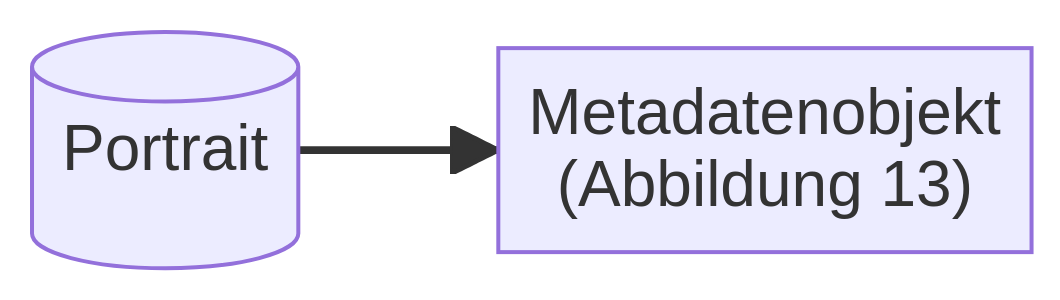
\includegraphics[width=2.85in,height=0.8in]{handbuch-diskriminierungsfreie-metadaten_files/figure-latex/mermaid-figure-6.png}

\textsubscript{Quelle:
\href{https://maehr.github.io/diskriminierungsfreie-metadaten/handbuch-diskriminierungsfreie-metadaten.qmd.html}{Artikel-Notizbuch}}

}

\caption{\label{fig-metadata-1}Ein Metadatenobjekt (Abbildung 13) hat
eine zugeordnete Ressource, nämlich ein Portrait.}

\end{figure}%

Dieses Diagramm zeigt, dass ein Metadatenobjekt (Abbildung 13) eine
zugeordnete Ressource hat, nämlich ein Portrait.

\subsubsection{Ein Metadatenobjekt mit drei zugeordneten Ressourcen
(Triptychon)}\label{ein-metadatenobjekt-mit-drei-zugeordneten-ressourcen-triptychon}

Dieses Diagramm stellt dar, dass ein Metadatenobjekt (Abbildung 7) drei
zugeordnete Ressourcen hat: die linke, mittlere und rechte Seite eines
Triptychons.

\begin{figure}

\centering{

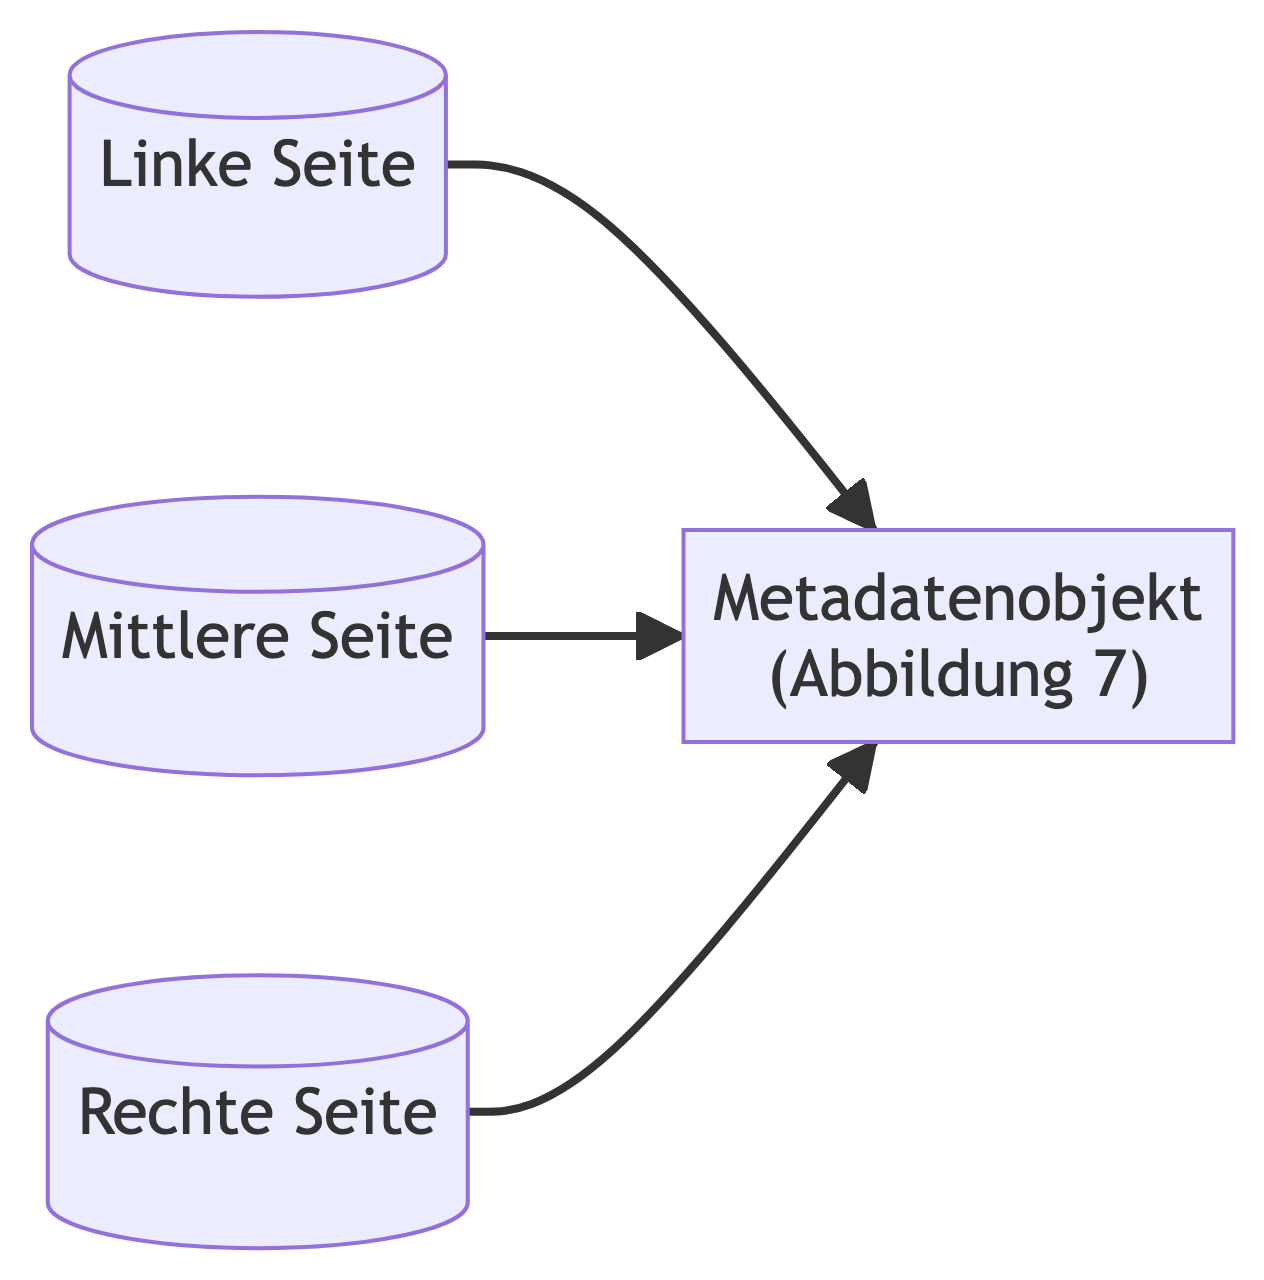
\includegraphics[width=3.3in,height=3.33in]{handbuch-diskriminierungsfreie-metadaten_files/figure-latex/mermaid-figure-10.png}

\textsubscript{Quelle:
\href{https://maehr.github.io/diskriminierungsfreie-metadaten/handbuch-diskriminierungsfreie-metadaten.qmd.html}{Artikel-Notizbuch}}

}

\caption{\label{fig-metadata-2}Ein Metadatenobjekt (Abbildung 7) hat
drei zugeordnete Ressourcen: die linke, mittlere und rechte Seite eines
Triptychons.}

\end{figure}%

\subsubsection{Ein Metadatenobjekt mit drei verschiedenen zugeordneten
Ressourcen}\label{ein-metadatenobjekt-mit-drei-verschiedenen-zugeordneten-ressourcen}

Hier sehen wir ein Metadatenobjekt (Abbildung 83) mit drei
unterschiedlichen zugeordneten Ressourcen: einer Karte, einer Legende
und Geodaten.

\begin{figure}

\centering{

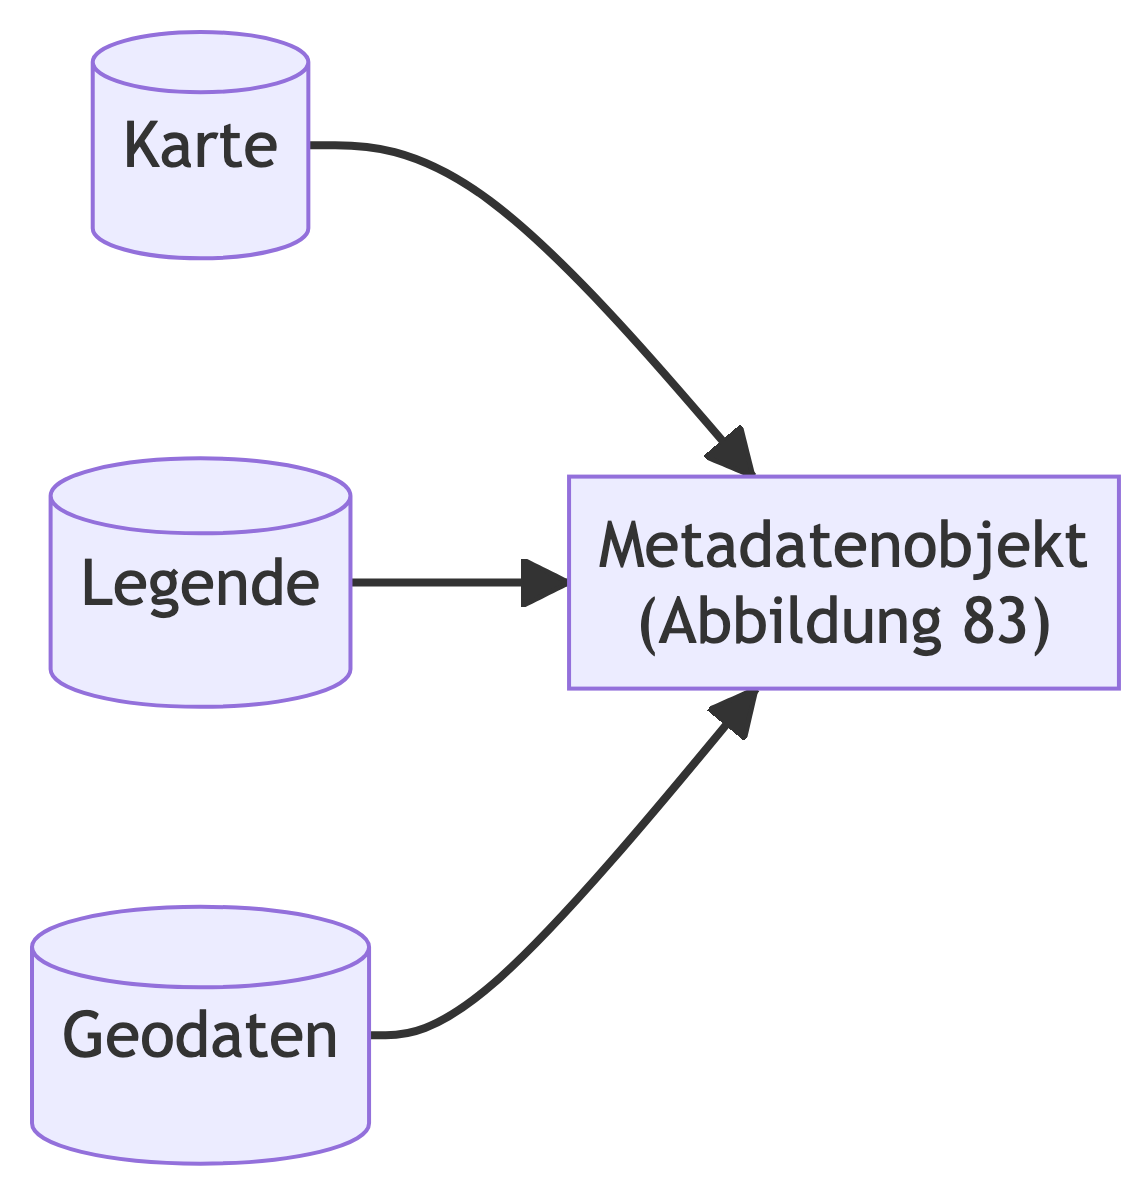
\includegraphics[width=3in,height=3.11in]{handbuch-diskriminierungsfreie-metadaten_files/figure-latex/mermaid-figure-9.png}

\textsubscript{Quelle:
\href{https://maehr.github.io/diskriminierungsfreie-metadaten/handbuch-diskriminierungsfreie-metadaten.qmd.html}{Artikel-Notizbuch}}

}

\caption{\label{fig-metadata-3}Ein Metadatenobjekt (Abbildung 83) hat
drei unterschiedliche zugeordnete Ressourcen: eine Karte, eine Legende
und Geodaten.}

\end{figure}%

\subsubsection{Zwei Metadatenobjekte mit derselben zugeordneten
Ressource}\label{zwei-metadatenobjekte-mit-derselben-zugeordneten-ressource}

Eine Abbildung wird zweimal verwendet. Folglich haben zwei
Metadatenobjekte (Abbildungen 73 und 11) dieselbe Ressource zugeordnet,
nämlich einen Kupferstich.

\begin{figure}

\centering{

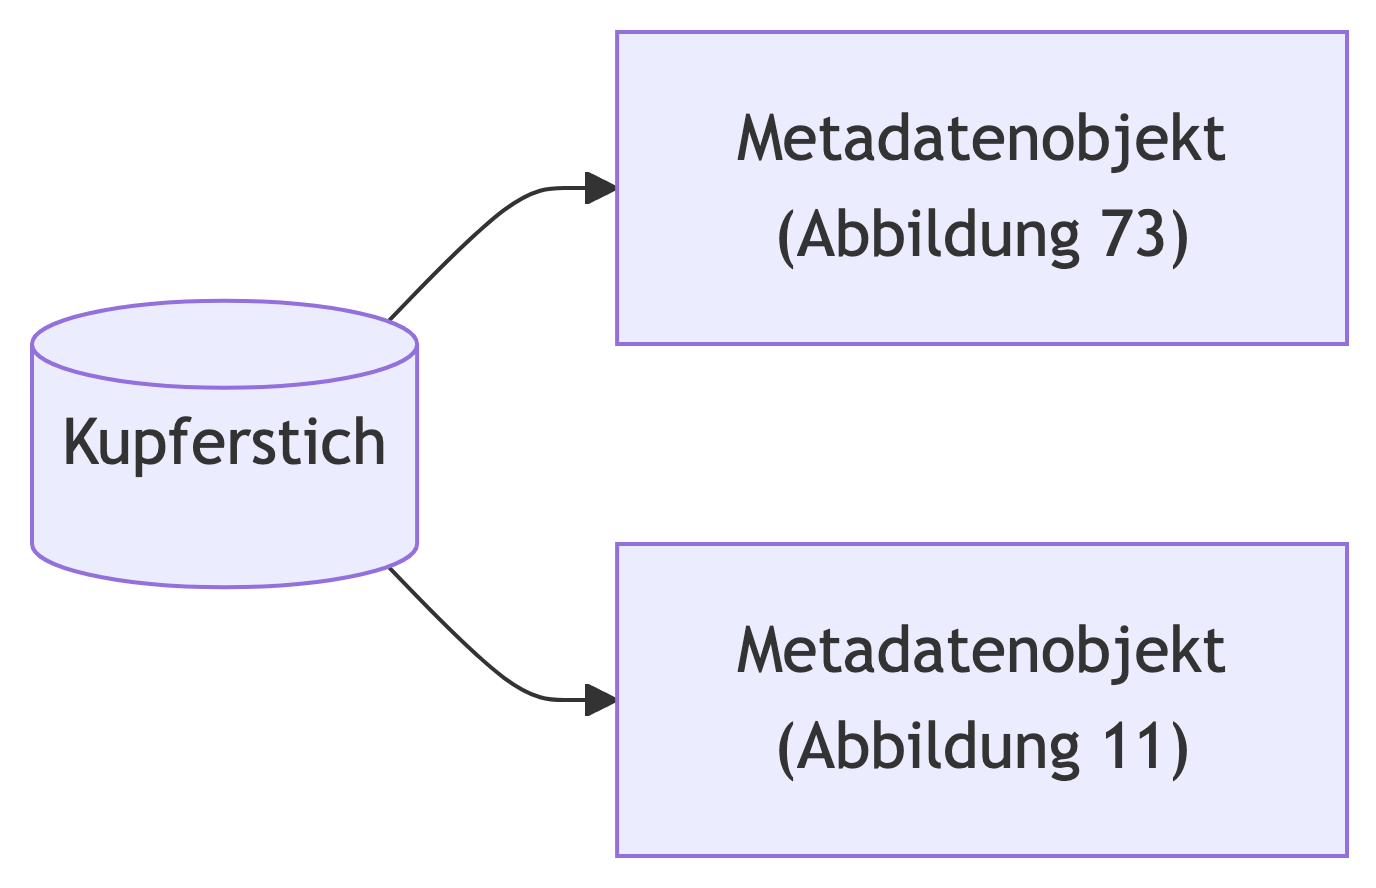
\includegraphics[width=3.12in,height=1.79in]{handbuch-diskriminierungsfreie-metadaten_files/figure-latex/mermaid-figure-8.png}

\textsubscript{Quelle:
\href{https://maehr.github.io/diskriminierungsfreie-metadaten/handbuch-diskriminierungsfreie-metadaten.qmd.html}{Artikel-Notizbuch}}

}

\caption{\label{fig-metadata-4}Zwei Metadatenobjekte mit derselben
zugeordneten Ressource}

\end{figure}%

\subsection{Metadatenobjekte (Eltern)}\label{metadatenobjekte-eltern}

\begin{longtable}[]{@{}
  >{\raggedright\arraybackslash}p{(\columnwidth - 8\tabcolsep) * \real{0.0221}}
  >{\raggedright\arraybackslash}p{(\columnwidth - 8\tabcolsep) * \real{0.0382}}
  >{\raggedright\arraybackslash}p{(\columnwidth - 8\tabcolsep) * \real{0.0262}}
  >{\raggedright\arraybackslash}p{(\columnwidth - 8\tabcolsep) * \real{0.2052}}
  >{\raggedright\arraybackslash}p{(\columnwidth - 8\tabcolsep) * \real{0.7082}}@{}}
\caption{Metadaten der Elternobjekte
(Metadatenobjekte).}\label{tbl-metadata-objects}\tabularnewline
\toprule\noalign{}
\begin{minipage}[b]{\linewidth}\raggedright
Name
\end{minipage} & \begin{minipage}[b]{\linewidth}\raggedright
Dublin Core
\end{minipage} & \begin{minipage}[b]{\linewidth}\raggedright
Obligatorisch
\end{minipage} & \begin{minipage}[b]{\linewidth}\raggedright
Verwendung
\end{minipage} & \begin{minipage}[b]{\linewidth}\raggedright
Datenwertstandard
\end{minipage} \\
\midrule\noalign{}
\endfirsthead
\toprule\noalign{}
\begin{minipage}[b]{\linewidth}\raggedright
Name
\end{minipage} & \begin{minipage}[b]{\linewidth}\raggedright
Dublin Core
\end{minipage} & \begin{minipage}[b]{\linewidth}\raggedright
Obligatorisch
\end{minipage} & \begin{minipage}[b]{\linewidth}\raggedright
Verwendung
\end{minipage} & \begin{minipage}[b]{\linewidth}\raggedright
Datenwertstandard
\end{minipage} \\
\midrule\noalign{}
\endhead
\bottomrule\noalign{}
\endlastfoot
ObjectID & dcterms:identifier & Ja & Eine eindeutige Zeichenfolge ohne
Leer- oder Sonderzeichen, die auf der Website als ID verwendet wird. &
Zufällig generierte Nummern zwischen abb000000 und abb999999. \\
Title & dcterms:title & Ja & Ein aussagekräftiger Name der Ressource. &
Keiner (Wenn möglich Übernahme aus Originalkatalog) \\
Subject & dcterms:subject & Ja & Die Schlagwörter der Ressource. &
\href{https://opengenderplatform.de/schlagwortindex}{Schlagwortindex
GenderOpen} Ein oder besser mehrere Schlagwörter, kommagetrennt. Für
Werte siehe Anhang Kapitel~\ref{sec-Schlagwortindex-GenderOpen}. \\
Description & dcterms:description & Ja & Eine Beschreibung der
Ressource. & Siehe Schritt-für-Schritt-Anleitung
Kapitel~\ref{sec-Schritt-für-Schritt-Anleitung} \\
Era & dcterms:temporal & Ja & Epoche (Frühgeschichte, Antike,
Mittelalter, Neuzeit, Zeitgeschichte)~ & `Ur- und
Frühgeschichte'`Römische Zeit und
Spätantike'`Mittelalter'`Neuzeit'`Zeitgeschichte'Auf eine Spezifikation
der
\href{https://www.dublincore.org/specifications/dublin-core/dcmi-period/}{Epochen
nach Dublin Core} wurde verzichtet, weil man sich zwischen den
verschiedenen Disziplinen nicht auf einheitliche Perioden einigen
konnte. \\
Is Part Of & dcterms:isPartOf & Ja & Eine verwandte Ressource, in der
die beschriebene Ressource physisch oder logisch enthalten ist. & DOI
oder bibliografische Angaben (nach
\href{https://www.infoclio.ch/de/zitierstil}{Infoclio Zitierstandard}),
mehrere Verweise können angegeben werden \\
\end{longtable}

\subsection{Zugeordnete Ressourcen
(Kinder)}\label{zugeordnete-ressourcen-kinder}

\begin{longtable}[]{@{}
  >{\raggedright\arraybackslash}p{(\columnwidth - 8\tabcolsep) * \real{0.0125}}
  >{\raggedright\arraybackslash}p{(\columnwidth - 8\tabcolsep) * \real{0.0215}}
  >{\raggedright\arraybackslash}p{(\columnwidth - 8\tabcolsep) * \real{0.0294}}
  >{\raggedright\arraybackslash}p{(\columnwidth - 8\tabcolsep) * \real{0.2276}}
  >{\raggedright\arraybackslash}p{(\columnwidth - 8\tabcolsep) * \real{0.7089}}@{}}
\caption{Metadaten der zugeordneten Ressourcen
(Kinder).}\label{tbl-metadata-resources}\tabularnewline
\toprule\noalign{}
\begin{minipage}[b]{\linewidth}\raggedright
Name
\end{minipage} & \begin{minipage}[b]{\linewidth}\raggedright
Dublin Core
\end{minipage} & \begin{minipage}[b]{\linewidth}\raggedright
Obligatorisch
\end{minipage} & \begin{minipage}[b]{\linewidth}\raggedright
Verwendung
\end{minipage} & \begin{minipage}[b]{\linewidth}\raggedright
Datenwertstandard
\end{minipage} \\
\midrule\noalign{}
\endfirsthead
\toprule\noalign{}
\begin{minipage}[b]{\linewidth}\raggedright
Name
\end{minipage} & \begin{minipage}[b]{\linewidth}\raggedright
Dublin Core
\end{minipage} & \begin{minipage}[b]{\linewidth}\raggedright
Obligatorisch
\end{minipage} & \begin{minipage}[b]{\linewidth}\raggedright
Verwendung
\end{minipage} & \begin{minipage}[b]{\linewidth}\raggedright
Datenwertstandard
\end{minipage} \\
\midrule\noalign{}
\endhead
\bottomrule\noalign{}
\endlastfoot
MediaID & dcterms:identifier & Ja & Eine eindeutige Zeichenfolge ohne
Leer- oder Sonderzeichen, die auf der Website als ID verwendet wird. &
Zufällig generierte Nummern zwischen m000000 und m999999. \\
Is Part Of & dcterms:isPartOf & Ja & Eine verwandte Ressource, in der
die beschriebene Ressource physisch oder logisch enthalten ist. &
ObjectID (des Elternobjekts), DOI oder bibliografische Angaben (nach
\href{https://www.infoclio.ch/de/zitierstil}{Infoclio Zitierstandard}),
mehrere Verweise können angegeben werden \\
Filename & & Ja & Der vollständige Pfad/URL einer (oder mehreren)
Datei(en) inkl. der Dateierweiterung. & Keiner (Wenn möglich Übernahme
der Pfade vom System zur Verwaltung der Metadaten und der Ressourcen,
z.B. \href{https://omeka.org/}{Omeka}) \\
Title & dcterms:title & Ja & Ein aussagekräftiger Name der Ressource. &
Keiner (Wenn möglich Übernahme aus Originalkatalog) \\
Subject & dcterms:subject & Ja & Die Schlagwörter der Ressource. &
\href{https://opengenderplatform.de/schlagwortindex}{Schlagwortindex
GenderOpen} Ein oder besser mehrere Schlagwörter, kommagetrennt. Für
Werte siehe Anhang Kapitel~\ref{sec-Schlagwortindex-GenderOpen} \\
Description & dcterms:description & Ja & Eine Beschreibung der
Ressource. & Siehe Schritt-für-Schritt-Anleitung
Kapitel~\ref{sec-Schritt-für-Schritt-Anleitung} \\
Creator & dcterms:creator & Nein & Eine Entität (Autor*in), die in
erster Linie für die Erstellung der Ressource verantwortlich ist. &
Klarname und URL zu \href{https://www.wikidata.org/}{Wikidata.org}
(Laufend Werte sammeln und wenn möglich dieselben wiederverwenden) \\
Publisher & dcterms:publisher & Ja & Eine Einrichtung, die für die
Bereitstellung der Ressource verantwortlich ist. (Bei Büchern und
Buchausschnitten ist eine Bibliothek anzugeben. Die bibliografische
Referenz wird unter Rights vermerkt.) & Klarname und URL zu
\href{https://www.wikidata.org/}{Wikidata.org} (Laufend Werte sammeln
und wenn möglich dieselben wiederverwenden) \\
& & & & Klarname und URL zu
\href{https://www.wikidata.org/}{Wikidata.org} (Laufend Werte sammeln
und wenn möglich dieselben wiederverwenden) \\
& & & & `Historisches Musem Basel
\href{http://www.wikidata.org/entity/Q386286}{Q386286}' \\
& & & & `Staatsarchiv des Kantons Basel-Stadt
\href{https://www.wikidata.org/wiki/Q2324698}{Q2324698}' \\
& & & & `Universitätsbibliothek Basel
\href{http://www.wikidata.org/entity/Q81164649}{Q81164649}' \\
& & & & `Basler Mission
\href{http://www.wikidata.org/entity/Q20614250}{Q20614250}' \\
& & & & `Jüdisches Museum
\href{http://www.wikidata.org/entity/Q1551099}{Q1551099}' \\
Date & dcterms:date & Nein & Der Zeitpunkt oder Zeitraum der
(geschätzten) Erstellung der Ressource. &
\href{https://www.loc.gov/standards/datetime/}{Extended Date/Time Format
(EDTF)} \\
& & & & `2014-03-05' Typisches vollständiges Datum, JJJJ-MM-TT, muss
führende Nullen an Monat und Tag enthalten \\
& & & & `2014-03' Nur für den Monat angegeben; ``irgendwann im März
2014''. \\
& & & & `2014' Nur für das Jahr angegeben; ``irgendwann im Jahr
2014''. \\
& & & & `2014-21' Jahreszeit (nördliche Hemisphäre): 21=Frühling,
22=Sommer, 23=Herbst, 24=Winter \\
& & & & `2014\textasciitilde{}' Ungefähres Datum: ``Ungefähr 2014''. Die
genaue Interpretation von ``ungefähr'' ist nicht spezifiziert, aber +/-
2 der genauesten angegebenen Einheiten (in diesem Beispiel Jahre) ist
eine vernünftige Erwartung. \\
& & & & `2014?' Ungewisses Datum: ``Vielleicht 2014.'' Die Alternative
könnte alles andere sein. Damit sollte jedoch sparsam umgegangen werden,
denn das ``alles andere'' ist unerwünscht. Wenn eine Vorstellung von
einem Bereich möglicher Daten besteht, kann die Bereichsform verwendet
werden. \\
& & & & `{[}2012,2014{]}' Eines der angegebenen Daten. \\
& & & & `2XXX' Unbestimmte Ziffer(n) von rechts: Das Zeichen ``X'' kann
anstelle einer oder mehrerer Ziffern ganz rechts verwendet werden, um
anzuzeigen, dass der Wert dieser Ziffer in den folgenden Fällen nicht
spezifiziert ist: Beispiel 1 `201X', Beispiel 2 `20XX' Jahr angegeben,
Monat unspezifiziert in einem Jahr-Monat-Ausdruck (Monatsgenauigkeit),
Beispiel 3 `2004-XX' Jahr und Monat werden angegeben, der Tag wird in
einem Jahr-Monat-Tag-Ausdruck nicht angegeben (Tagesgenauigkeit),
Beispiel 4 `1985-04-XX' Jahr angegeben, Tag und Monat nicht angegeben in
einem Jahr-Monat-Tag-Ausdruck (Tagesgenauigkeit), Beispiel 5
`1985-XX-XX' \\
& & & & `{[}2014-01-03..2014-04-15{]}' Bereich des ungewissen Datums:
``Irgendwann zwischen dem 3. Januar und dem 15. April 2014.'' Beachte,
dass genau zwei Zeiträume zwischen den Daten liegen. Dies ist die
bevorzugte Form für unbestimmte Daten, da sie für den Computer am
einfachsten zu verarbeiten ist. NICHT ein Intervall gültiger Daten (``im
Zeitraum vom 3. Januar bis 15. April 2014''); das wird als separates
Start- und Enddatum eingegeben. \\
& & & & `{[}..2014-04-15{]}' Unbegrenzter Bereich mit ungewissem Datum:
``Irgendwann vor dem 15. April 2014''. Wenn du also eine Vorstellung vom
Beginn des Zeitfensters hast, gib es bitte ein. \\
& & & & `{[}2014-04-15..{]}' Offener Bereich mit ungewissem Datum:
``Irgendwann nach dem 15. April 2014''. Das System interpretiert dies
als einen Zeitpunkt zwischen diesem Datum und heute. Wenn du also eine
Vorstellung vom Ende des Zeitfensters hast, gib es bitte ein. \\
& & & & `unknown' Das Datum ist völlig unbekannt, aber es ist bekannt,
dass das Ereignis an einem bestimmten Datum stattfindet. Wir wissen
z.B., dass die Organisation eines Zweigs an einem bestimmten Tag
stattgefunden haben muss, aber wir haben keine Ahnung, wann dieser Tag
war. Bitte gehe sparsam damit um, denn das System kann daraus nichts
abschätzen; wenn du eine Vorstellung von einem bestimmten Datum hast,
verwende das Formular für den Zeitraum. \\
Era & dcterms:temporal & Ja & Epoche (Frühgeschichte, Antike,
Mittelalter, Neuzeit, Zeitgeschichte) & `Ur- und Frühgeschichte' \\
& & & & `Römische Zeit und Spätantike' \\
& & & & `Mittelalter' \\
& & & & `Neuzeit' \\
& & & & `Zeitgeschichte' \\
& & & & Auf eine Spezifikation der
\href{https://www.dublincore.org/specifications/dublin-core/dcmi-period/}{Epochen
nach Dublin Core} wurde verzichtet, weil man sich zwischen den
verschiedenen Disziplinen nicht auf einheitliche Perioden einigen
konnte. \\
Type & dcterms:type & Ja & Die Art oder das Genre der referenzierten
Ressource im Archiv/Bibliothek etc. &
\href{https://www.dublincore.org/specifications/dublin-core/dcmi-terms/\#section-7}{DCMI
Type Vocabulary} \\
& & & & Bei Grafiken wird zu Zwecken einer semantischen Klarheit anstatt
``Dataset'' den Type ``Image'' verwendet. \\
& & & & `Collection' Eine Sammlung von Ressourcen. \\
& & & & `Dataset' Eine Sammlung von Daten, die für die Verarbeitung
durch ein Computerprogramm strukturiert ist. \\
& & & & `Event' Eine zeitliche Entität, die durch einen festen Zeitpunkt
oder ein Intervall im Zeitverlauf gekennzeichnet ist. \\
& & & & `Image' Eine visuelle Darstellung, die nicht primär für
Kommunikation über Text hinausgeht. \\
& & & & `Interactive Resource' Eine Ressource, die eine Interaktion mit
dem Benutzer erfordert, um ihren Zweck zu erfüllen. \\
& & & & `Moving Image' Eine Serie von visuellen Darstellungen, die eine
Illusion von Bewegung erzeugen, wenn sie in schneller Abfolge gezeigt
werden. \\
& & & & `Physical Object' Ein physisches Objekt (z.B. ein Buch, ein
Gemälde oder eine Statue). \\
& & & & `Service' Ein System, das anderen Systemen Ressourcen zur
Verfügung stellt. \\
& & & & `Software' Ein Computerprogramm in ausführbarer Form. \\
& & & & `Sound' Eine Ressource, die primär für die Wahrnehmung durch das
Ohr bestimmt ist. \\
& & & & `Still Image' Eine statische visuelle Darstellung. \\
& & & & `Text' Eine Ressource, die primär für die Kommunikation durch
Text bestimmt ist. \\
Format & dcterms:format & Ja & Das Dateiformat der Ressource. &
\href{http://www.iana.org/assignments/media-types/}{Internet Media Types
(MIME)} \\
& & & & `application/pdf' Portable Document Format (PDF). \\
& & & & `image/jpeg' JPEG-Bilddateien. \\
& & & & `image/png' PNG-Bilddateien. \\
& & & & `image/gif' GIF-Bilddateien. \\
& & & & `image/svg+xml' SVG (Scalable Vector Graphics) Dateien. \\
& & & & `audio/mpeg' MP3-Audiodateien. \\
& & & & `audio/wav' WAV-Audiodateien. \\
& & & & `video/mp4' MP4-Videodateien. \\
Extent & dcterms:extent & Nein & Das physische Medium oder die
Abmessungen der Ressource. & Breite und Höhe in Pixel (kann
automatisiert aus der Bilddatei ausgelesen werden) \\
Source & dcterms:source & Ja (ausser Abbildungen) & Ein eindeutiger
Verweis auf die Ressource innerhalb eines bestimmten Kontexts. &
Institutionenspezifisch (Wenn möglich Übernahme aus Originalkatalog) \\
Language & dcterms:language & Nein & Eine Sprache der Ressource. &
\href{https://www.loc.gov/standards/iso639-2/php/code_list.php}{ISO
639-2} \\
Relation & dcterms:relation & Ja (ausser Privatsammlung) & Eine
verwandte Ressource. & URL zum Originalkatalog \\
Rights & dcterms:rights & Ja & Informationen über die Rechte an der
Ressource. Achtung: Bei Fotografien ist die Fotograf:in ebenfalls hier
anzugeben. & Keiner (Wenn möglich Übernahme aus Originalkatalog) \\
License & & Ja & URL zur Lizenz &
\href{https://creativecommons.org/}{CreativeCommons.org} oder
\href{https://rightsstatements.org/en/}{RightsStatements.org} \\
& & & & `\url{https://creativecommons.org/publicdomain/mark/1.0/}'
Public Domain Mark (PDM)
\href{https://creativecommons.org/public-domain/freeworks/}{\emph{{[}Free
Culture{]}}} \\
& & & & `\url{https://creativecommons.org/publicdomain/zero/1.0/}' CC0
\href{https://creativecommons.org/public-domain/freeworks/}{\emph{{[}Free
Culture{]}}} \\
& & & & `\url{https://creativecommons.org/licenses/by/4.0/}' CC BY
(Attribution)
\href{https://creativecommons.org/public-domain/freeworks/}{\emph{{[}Free
Culture{]}}} Erlaubt anderen, das Werk zu verbreiten, zu remixen, zu
verändern und darauf aufzubauen, auch kommerziell, solange der Urheber
genannt wird. \\
& & & & `\url{https://creativecommons.org/licenses/by-sa/4.0/}' CC BY-SA
(Attribution-ShareAlike)
\href{https://creativecommons.org/public-domain/freeworks/}{\emph{{[}Free
Culture{]}}} Erlaubt anderen, das Werk zu remixen, zu verändern und
darauf aufzubauen, auch kommerziell, solange das neue Werk unter der
gleichen Lizenz veröffentlicht wird. \\
& & & & `\url{https://creativecommons.org/licenses/by-nc-sa/4.0/}' CC
BY-NC-SA (Attribution-NonCommercial-ShareAlike) Erlaubt anderen, das
Werk zu bearbeiten, solange es nicht kommerziell genutzt wird und unter
denselben Bedingungen weitergegeben wird. \\
& & & & `\url{http://rightsstatements.org/vocab/InC/1.0/}' In Copyright.
Das Werk ist urheberrechtlich geschützt. \\
& & & & `\url{http://rightsstatements.org/vocab/InC-RUU/1.0/}' In
Copyright - Rights-holder(s) unlocatable or unidentifiable \\
\end{longtable}

\subsection{Relation von Objekt und
Media}\label{relation-von-objekt-und-media}

\begin{figure}

\centering{

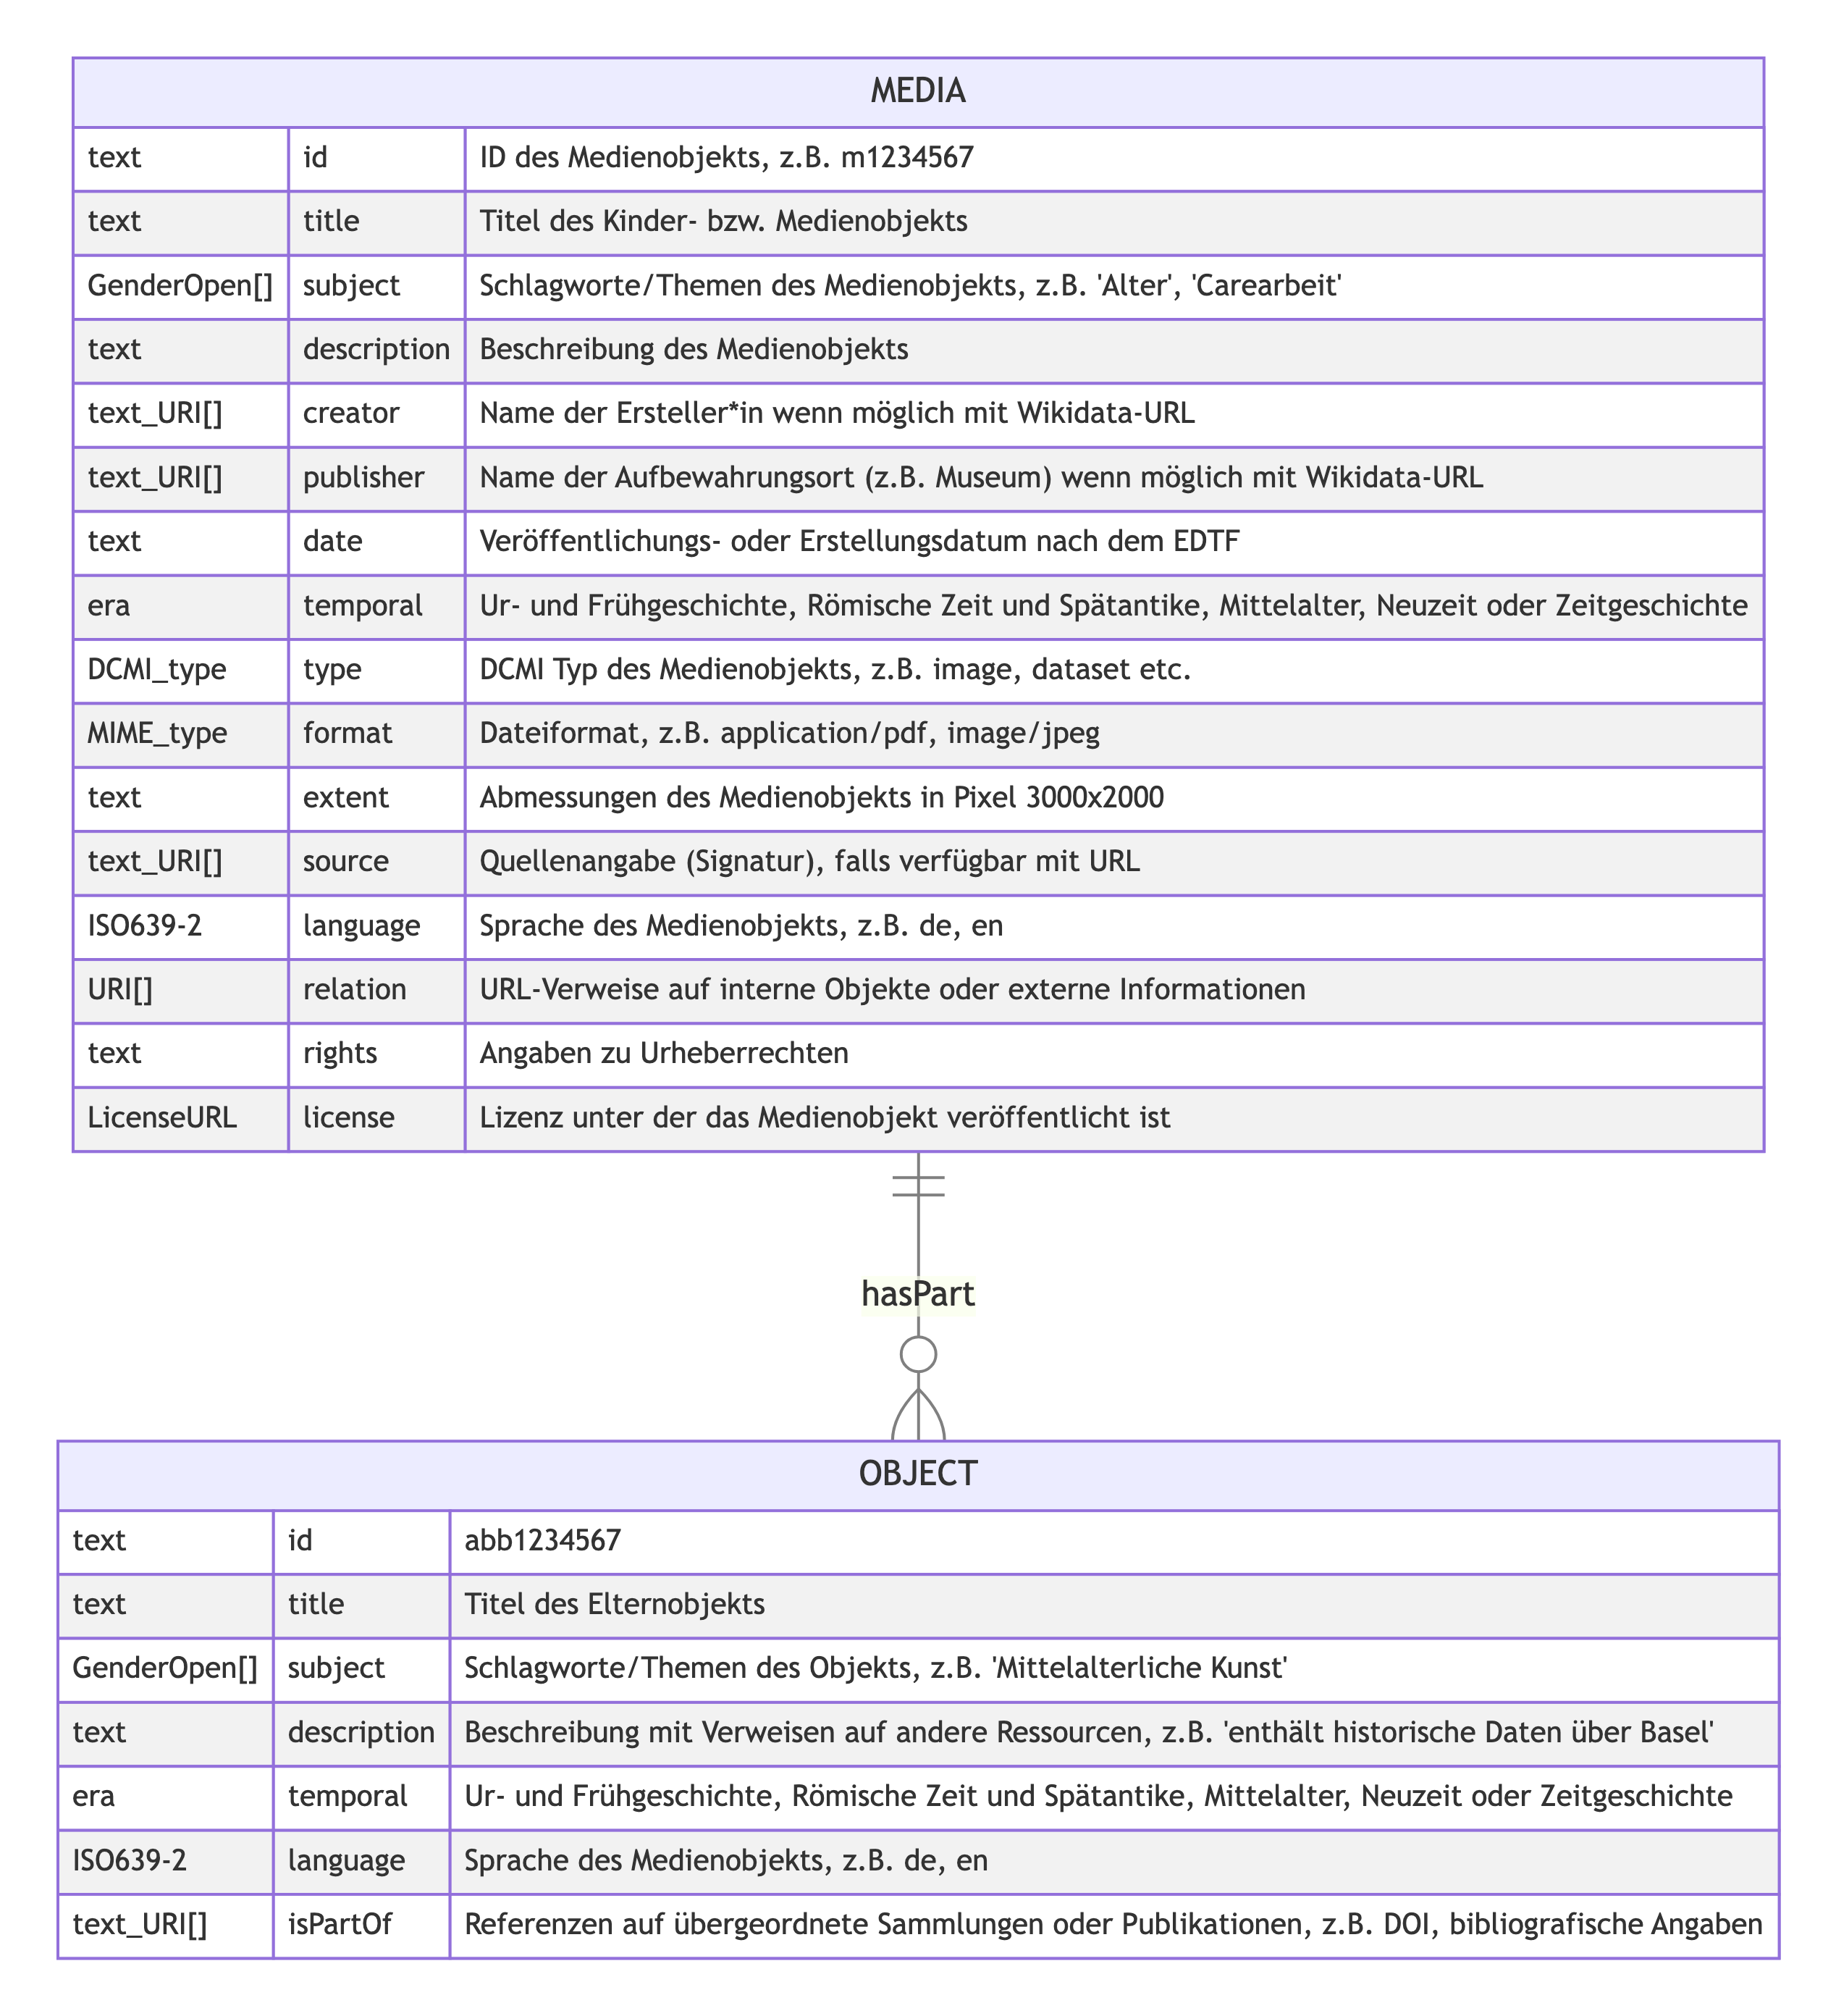
\includegraphics[width=6.61in,height=7.25in]{handbuch-diskriminierungsfreie-metadaten_files/figure-latex/mermaid-figure-7.png}

\textsubscript{Quelle:
\href{https://maehr.github.io/diskriminierungsfreie-metadaten/handbuch-diskriminierungsfreie-metadaten.qmd.html}{Artikel-Notizbuch}}

}

\caption{\label{fig-metadata-5}Relation von Objekt und Media.}

\end{figure}%

\section{Schritt-für-Schritt-Anleitung zur Erstellung von~Metadaten für
historische Quellen und
Forschungsdaten}\label{sec-Schritt-fuxfcr-Schritt-Anleitung}

In diesem Kapitel wird eine detaillierte Anleitung zur Erstellung von
Metadaten für historische Ressourcen präsentiert, wobei ein besonderer
Fokus auf dem Umgang mit sensiblen Inhalten liegt. Die Anleitung
beinhaltet bewährte Praktiken aus der bestehenden Fachliteratur sowie
Erfahrungen, die im Rahmen von Stadt.Geschichte.Basel gesammelt wurden.
Dabei werden nicht nur allgemeine Tipps zum Umgang mit Metadaten
gegeben, sondern auch konkrete Schritte und Herausforderungen aus dem
Projekt Stadt.Geschichte.Basel illustriert. Die Erfahrungen sind jeweils
in den grauen Kästen vermerkt. Diese Schritt-für-Schritt-Anleitung dient
sowohl Personen, die sich neu mit Metadaten befassen, als auch
erfahrenen Fachpersonen als Ressource für die Gestaltung der Metadaten.

\subsection{Erster Schritt:
Vorbereitung}\label{erster-schritt-vorbereitung}

Der erste Schritt besteht darin, zu klären, welche Metadaten zu welchem
Zweck und für welches Publikum gesammelt werden sollen. Die folgenden
Fragen über die Art der Ressource, die Zielgruppe oder den Kontext
helfen bei der Eingrenzung der relevanten Metadaten.

\subsubsection{Was beschreibe ich?}\label{was-beschreibe-ich}

Wird ein physisches Objekt, ein digitales Objekt oder eine digitale
Darstellung eines physischen Objekts beschrieben? Diese Frage ist
wichtig, da unterschiedliche Arten von Quellen unterschiedliche
Informationen erfordern und spezifische Metadatenkategorien relevant
sein können. Die grundlegenden Unterschiede sind:

\begin{itemize}
\tightlist
\item
  Physische Objekte sind materielle Gegenstände wie Bücher, Gemälde,
  Dokumente oder Artefakte. Beim Erstellen von Metadaten für physische
  Objekte müssen Informationen erfasst werden, die direkt mit dem Objekt
  selbst in Verbindung stehen. Dazu gehören physische Merkmale wie
  Grösse, Material, Zustand, Herkunft und allenfalls spezielle Merkmale
  oder Besonderheiten des Objekts.
\item
  Digitale Objekte sind nicht-materielle Inhalte, die in digitaler Form
  vorliegen. Sie können unter anderem Texte, Bilder, Audio- oder
  Videodateien umfassen. Bei den Metadaten für digitale Objekte müssen
  technische Informationen wie Dateiformat und -typ, Dateigrösse oder
  Auflösung berücksichtigt werden. Ausserdem müssen Rechte und Lizenzen
  des digitalen Objektes geklärt und entsprechende Informationen zu
  Urheberrechten angegeben werden.
\item
  Digitale Darstellungen physischer Objekte sind digitale
  Repräsentationen von physischen Objekten. Bei der Erstellung von
  Metadaten für digitale Darstellungen physischer Objekte müssen sowohl
  Informationen über das ursprüngliche physische Objekt als auch über
  die digitalen Aspekte erfasst werden.
\end{itemize}

\begin{tcolorbox}[enhanced jigsaw, breakable, bottomtitle=1mm, left=2mm, opacitybacktitle=0.6, coltitle=black, toprule=.15mm, arc=.35mm, colframe=quarto-callout-tip-color-frame, titlerule=0mm, rightrule=.15mm, toptitle=1mm, title=\textcolor{quarto-callout-tip-color}{\faLightbulb}\hspace{0.5em}{Erfahrungen der Stadt.Geschichte.Basel}, bottomrule=.15mm, leftrule=.75mm, opacityback=0, colbacktitle=quarto-callout-tip-color!10!white, colback=white]

Bei den Ressourcen der Stadt.Geschichte.Basel handelt es sich vorwiegend
um digitale Darstellungen physischer Objekte sowie um digitale Objekte.
Vor diesem Hintergrund muss der Fokus bezüglich der Metadaten von Anfang
an breit gesetzt werden. Das hat dazu geführt, dass im Verlauf des
Erstellens des Metadatenschemas einzelne Felder hinzugefügt und später
wieder verworfen wurden.

\end{tcolorbox}

\subsubsection{Wer ist meine
Zielgruppe?}\label{wer-ist-meine-zielgruppe}

Es ist wichtig, die Zielgruppe für die zu erstellenden Metadaten zu
kennen, da sie die Relevanz, den Umfang und die Art der Metadaten
beeinflusst. Auch die Zielgruppe, die auf die Metadaten zugreift, kann
von Diskriminierungserfahrungen betroffen sein. Das muss berücksichtigt
werden. Durch die Kenntnis der Zielgruppe können die Metadaten
spezifisch auf die Bedürfnisse der Benutzer*innen angepasst werden.

\begin{tcolorbox}[enhanced jigsaw, breakable, bottomtitle=1mm, left=2mm, opacitybacktitle=0.6, coltitle=black, toprule=.15mm, arc=.35mm, colframe=quarto-callout-tip-color-frame, titlerule=0mm, rightrule=.15mm, toptitle=1mm, title=\textcolor{quarto-callout-tip-color}{\faLightbulb}\hspace{0.5em}{Erfahrungen der Stadt.Geschichte.Basel}, bottomrule=.15mm, leftrule=.75mm, opacityback=0, colbacktitle=quarto-callout-tip-color!10!white, colback=white]

Die Hauptzielgruppe umfasst Forschende und Studierende, die nebst
technischen Informationen auch Metadaten benötigen, die ihnen dabei
helfen, den Kontext der Forschungsdaten zu verstehen. Beispiele dafür
sind etwa Informationen über den historischen Zeitraum, die kulturellen
oder politischen Bedingungen sowie die Quellenbasis.

\end{tcolorbox}

\subsubsection{Welche Informationen werden benötigt, um die Ressource zu
identifizieren?}\label{welche-informationen-werden-benuxf6tigt-um-die-ressource-zu-identifizieren}

Dies kann je nach Informationsstand und Art der Objekte mehr oder
weniger Zeit in Anspruch nehmen. Es ist wichtig, mögliche
Schwierigkeiten bei der Identifizierung von Beginn weg zu
berücksichtigen. Beispielsweise können unvollständige oder beschädigte
Informationen, wie beispielsweise verblasste Beschriftungen, die
Identifizierung physischer Objekte erschweren.

\begin{tcolorbox}[enhanced jigsaw, breakable, bottomtitle=1mm, left=2mm, opacitybacktitle=0.6, coltitle=black, toprule=.15mm, arc=.35mm, colframe=quarto-callout-tip-color-frame, titlerule=0mm, rightrule=.15mm, toptitle=1mm, title=\textcolor{quarto-callout-tip-color}{\faLightbulb}\hspace{0.5em}{Erfahrungen der Stadt.Geschichte.Basel}, bottomrule=.15mm, leftrule=.75mm, opacityback=0, colbacktitle=quarto-callout-tip-color!10!white, colback=white]

Stadt.Geschichte.Basel war bei der Identifikation der Informationen für
die Ressourcen mit folgenden Schwierigkeiten konfrontiert: Insbesondere
bei Archiven fehlten oftmals Beschreibungen zu einzelnen Ressourcen.
Konkret fehlte etwa beim Plakat zu den sogenannten "Völkerschauen"
(siehe Kapitel~\ref{sec-plakat-zur-voelkerschau}) die Information, wer
das Plakat herstellte. In solchen Fällen waren selbständige Recherchen
oder eine Rücksprache mit den jeweiligen Gedächtnisinstitutionen
erforderlich.

\end{tcolorbox}

\subsubsection{Welche Informationen werden benötigt, um die Ressourcen
in den richtigen Kontext zu
setzen?}\label{welche-informationen-werden-benuxf6tigt-um-die-ressourcen-in-den-richtigen-kontext-zu-setzen}

Um eine Ressource kontextualisieren zu können, müssen grundlegende
Aspekte wie der historische Zeitraum, der geografische Kontext, der
kulturelle und soziale Hintergrund sowie die Quellenbasis berücksichtigt
werden. Mit der Kontextualisierung der historischen Ressource wird
sichergestellt, dass die Ressource nicht isoliert betrachtet, sondern in
einen grösseren historischen, sozialen und politischen Kontext gestellt
wird.

\begin{tcolorbox}[enhanced jigsaw, breakable, bottomtitle=1mm, left=2mm, opacitybacktitle=0.6, coltitle=black, toprule=.15mm, arc=.35mm, colframe=quarto-callout-tip-color-frame, titlerule=0mm, rightrule=.15mm, toptitle=1mm, title=\textcolor{quarto-callout-tip-color}{\faLightbulb}\hspace{0.5em}{Erfahrungen der Stadt.Geschichte.Basel}, bottomrule=.15mm, leftrule=.75mm, opacityback=0, colbacktitle=quarto-callout-tip-color!10!white, colback=white]

Stadt.Geschichte.Basel legt besonderen Wert auf die Kontextualisierung,
um nicht unkritisch Diskriminierung in einzelnen Ressourcen zu
reproduzieren. Für die Recherche stützt sich Stadt.Geschichte.Basel
unter anderem auf Informationen aus den Bänden des Projekts sowie auf
historische Nachschlagewerke wie das
\href{https://www.baslerstadtbuch.ch/home.html}{Basler Stadtbuch} oder
das \href{https://hls-dhs-dss.ch/}{Historische Lexikon der Schweiz}. Um
eine weiterführende Recherche zu ermöglichen und zu erleichtern, sind
die entsprechenden Nachschlagewerke im Fliesstext der
Quellenbeschreibung direkt verlinkt.

\end{tcolorbox}

Im untenstehenden Beispiel aus den Ressourcen der Stadt.Geschichte.Basel
werden die Schritte zur Kontextualisierung einer Quelle ausgeführt.

\subsubsection{Beispiel: Beschreibung der Reproduktion des Plakates
"Völkerschau in Basel
1926"}\label{beispiel-beschreibung-der-reproduktion-des-plakates-vuxf6lkerschau-in-basel-1926}

Im Zeitraum zwischen 1879 und 1935 fanden im Basler Zoo 21 sogenannte
``\href{https://www.baslerstadtbuch.ch/stadtbuch/1992/1992_2247.html}{Völkerschauen''
(Achtung Link führt zu diskriminierenden Bildern)} --- heute auch
Menschenzoos genannt --- statt, in denen Menschen aus verschiedenen
Kulturen ausgestellt wurden. Schweizweit fanden solche Schauen bis ins
Jahr 1964 statt. Bei diesen Veranstaltungen wurden Menschen entweder in
festen Einrichtungen, mobilen Zoos oder sogar in Zirkusvorführungen zur
Schau gestellt. Dahinter stand ein rassistisches, imperialistisches und
kolonialistisches Menschenbild. Die in den Werbeplakaten verwendete
Bildsprache bediente sich an kolonialen Fantasien der europäischen
Bevölkerung und stellte die Menschen als vermeintlich''primitiv'',
``wild'', ``kriegerisch'' und ``exotisch'' dar, was zu einer
Aufrechterhaltung von negativen Stereotypen führte. Die Schauen waren in
der Ideologie der ``Rassentheorie'' verwurzelt, die eine Überlegenheit
der europäischen Bevölkerung gegenüber anderen Kulturen auf angeblich
wissenschaftlicher Grundlage behauptete. Die Ideologie der
\href{https://hls-dhs-dss.ch/de/articles/060537/2024-04-08/}{Rassentheorie}
wurde genutzt, um die Ausstellung dieser Menschen als akzeptabel
darzustellen, indem sie als blosse Objekte zur Unterhaltung des
Publikums behandelt wurden. Die tief verwurzelten Stereotypen und
Vorurteile wurden über Generationen hinweg in
\href{https://mirsindvoda.ch/voelkerschauen-in-der-schweiz/}{Kultur und
Sprache} weitergegeben, sei es durch Bücher, Filme oder Erzählungen.
Einige der Bilder, die einst dazu gedient haben sollen, die
Unterdrückung oder vermeintliche "Rettung" und den "Schutz vor sich
selbst" bestimmter "primitiver und unzivilisierter Völker" zu
rechtfertigen, bestehen teilweise noch bis heute und manifestieren sich
in unterschiedlichen Formen von Diskriminierung.

In die Beschreibung~der Reproduktion des Plakates "Völkerschau in Basel
1926" (siehe Kapitel~\ref{sec-plakat-zur-voelkerschau})~sind folgende
Überlegungen eingeflossen:

\paragraph{Entstehungskontext der
Ressource}\label{entstehungskontext-der-ressource}

Zunächst ist es wichtig, die Ressource in einen historischen Kontext zu
stellen. Rassistische Ideologien haben sich im Laufe der Geschichte
verändert, und auch das Verständnis von Rassismus hat sich gewandelt.
Daher ist es wichtig, die Ressource im Kontext ihrer Entstehungszeit zu
analysieren, um zu verstehen, wie rassistische Überzeugungen zu dieser
Zeit verbreitet waren.

\subparagraph{Sozialer und politischer
Kontext}\label{sozialer-und-politischer-kontext}

Diskriminierungsformen wie Rassismus sind eng mit sozialen, politischen,
wissenschaftlichen, ökonomischen und kulturellen Strukturen verbunden.
Die Auseinandersetzung mit dem gesellschaftlichen und politischen
Kontext ermöglicht es, Faktoren wie rechtliche und soziale
Diskriminierung, koloniale Herrschaftssysteme, diskriminierende
Rezeptions- und Reproduktionspraktiken sowie allgemeine institutionelle
Strukturen zu erkennen. Dieses Wissen hilft auch, die Motivation hinter
Darstellungen wie dem Plakat des Basler Zoos besser einzuschätzen und
kritisch zu hinterfragen.

\subparagraph{Quellenbeschreibung}\label{quellenbeschreibung}

Zu jeder Kontextualisierung gehört eine inhaltliche Beschreibung der
Quelle, um die spezifischen Diskriminierungsformen zu benennen. Auch die
Intention der Quelle ist für das Verständnis des Kontextes notwendig. Im
Fall des oben beschriebenen Beispiels wurde das Plakat unter anderem
deshalb erstellt, um einem weissen Publikum die Sensation anzupreisen,
eine vermeintlich ``primitive'' und ``exotischen'' Bevölkerungsgruppe
sehen zu können.

\subparagraph{Kontext der Autor*innen}\label{kontext-der-autorinnen}

Informationen über die Verfasser*innen der Quelle können ebenfalls dazu
beitragen, Aufschluss darüber zu geben, warum bestimmte
Diskriminierungsformen in der Quelle dargestellt werden. Fragen wie "Wer
war die Person?" "Was war ihre Position?" "Welche Überzeugungen könnten
ihre Sichtweise beeinflusst haben?" können gestellt werden.

\subparagraph{Interpretation und
Rezeption}\label{interpretation-und-rezeption}

Bei der Kontextualisierung ist es wichtig, die historische
Interpretation und Rezeption zu berücksichtigen. Wie wurde die Quelle
zur Zeit ihrer Entstehung von der breiten Öffentlichkeit interpretiert?
Wie wird sie heute interpretiert? Welche Kontroversen oder Diskussionen
gab es um die Quelle? Es ist wichtig, immer die historische und die
gegenwärtige Seite gegenüber zu stellen sowie auf Kontinuitäten von
Diskriminierungsformen hinzuweisen, um die Quelle richtig bewerten zu
können und vor allem, um die Diskriminierung, die sie enthält, besser
aufzeigen zu können.

\subparagraph{Begriffe}\label{begriffe}

In den letzten Jahren hat die öffentliche Debatte, wie mit
diskriminierenden Begriffen in Metadaten umgegangen werden soll,
zugenommen. Auch Museen, Archive und Bibliotheken stellen sich vermehrt
die Frage, welche Methoden angewendet werden sollen, damit
Diskriminierung nicht reproduziert wird. Im Folgenden werden drei
unterschiedliche Ansätze erläutert. Bei der ``Titelkontextualisierung''
wird zwar der diskriminierende Begriff benannt, aber gleichzeitig
kritisch kontextualisiert, wobei der Umfang der Kontextualisierung stark
variieren kann. Ein anderer Ansatz ist die ``Titelverfremdung''. Dabei
können die Titel auf den Kopf gestellt, durchgestrichen oder gespiegelt
werden. Ausserdem ist die Einbindung von Sternchen möglich, bei der die
einzelnen Buchstaben durch Asterisken ersetzt werden. Als dritte Methode
kann der Titel geändert werden. Wichtig ist dabei, diesen Prozess der
Titeländerung zu dokumentieren. Warum wurde der Begriff geändert und wer
hat dem Objekt seinen Titel gegeben? Zudem ist es für die
Objektgeschichte oder Sammlungsgeschichte nicht unwichtig, aus welcher
Perspektive das Objekt rezipiert wurde und aus welcher Motivation das
Objekt gesammelt wurde.

\begin{tcolorbox}[enhanced jigsaw, breakable, bottomtitle=1mm, left=2mm, opacitybacktitle=0.6, coltitle=black, toprule=.15mm, arc=.35mm, colframe=quarto-callout-tip-color-frame, titlerule=0mm, rightrule=.15mm, toptitle=1mm, title=\textcolor{quarto-callout-tip-color}{\faLightbulb}\hspace{0.5em}{Erfahrungen der Stadt.Geschichte.Basel}, bottomrule=.15mm, leftrule=.75mm, opacityback=0, colbacktitle=quarto-callout-tip-color!10!white, colback=white]

Das Projekt hat sich für die Methode der ``Titelkontextualisierung''
entschieden - unter anderem wegen der besseren Durchsuchbarkeit auf der
\href{https://forschung.stadtgeschichtebasel.ch/}{Forschungsdatenplattform}.
Weil der Schlagwortindex-GenderOpen gezielt sensible Schlagworte
enthält, lassen sich Diskriminierungen in historischen Quellen einfacher
finden. Die diskriminierenden Inhalte werden auf der Webseite jeweils
mit einer Triggerwarnung angezeigt.

\end{tcolorbox}

\subsubsection{Wie werden die Metadaten der Zielgruppe zugänglich
gemacht?}\label{wie-werden-die-metadaten-der-zielgruppe-zuguxe4nglich-gemacht}

Es gibt eine Vielzahl von Möglichkeiten, Metadaten der Zielgruppe
zugänglich zu machen. So können Metadaten etwa in öffentlichen
Bibliotheken, Archiven oder Online-Archiven - sogenannten Repositorien -
veröffentlicht werden. Wichtig ist hierbei zu beachten, dass bei Open
Data Plattformen nicht immer kontrolliert werden kann, wer und wie die
Metadaten verwendet werden.

\begin{tcolorbox}[enhanced jigsaw, breakable, bottomtitle=1mm, left=2mm, opacitybacktitle=0.6, coltitle=black, toprule=.15mm, arc=.35mm, colframe=quarto-callout-tip-color-frame, titlerule=0mm, rightrule=.15mm, toptitle=1mm, title=\textcolor{quarto-callout-tip-color}{\faLightbulb}\hspace{0.5em}{Erfahrungen der Stadt.Geschichte.Basel}, bottomrule=.15mm, leftrule=.75mm, opacityback=0, colbacktitle=quarto-callout-tip-color!10!white, colback=white]

Stadt.Geschichte.Basel betreibt eine
\href{https://forschung.stadtgeschichtebasel.ch/}{Forschungsdatenplattform}.~Diese
wird als zentrales Repositorium dienen, in dem alle Forschungsressourcen
gesammelt und für die Öffentlichkeit nach den FAIR-Prinzipien zugänglich
gemacht werden. Nutzer*innen können einfach auf die Plattform zugreifen,
die umfangreiche Datenbank durchsuchen und relevante Ressourcen für ihre
spezifischen Bedürfnisse finden.~Daher ist es wichtig, klare und präzise
Informationen darüber zu liefern, wem diese Ressourcen gehören und wer
sie nutzen kann. Die Details zu Eigentum und Nutzungsrechten werden
deutlich in den Metadaten jeder Ressource angegeben.

\end{tcolorbox}

\subsection{Schritt Zwei: Metadatenfelder
festlegen}\label{schritt-zwei-metadatenfelder-festlegen}

Für die Festlegung der Metadatenfelder empfiehlt es sich, von einem
Standard auszugehen und die Liste entsprechend der eigenen Bedürfnisse
anzupassen.

Stadt.Geschichte.Basel ist von den 15 Feldern vom
\href{https://www.dublincore.org/specifications/dublin-core/dces/}{Dublin
Core Metadata Element Set} ausgegangen:

\begin{longtable}[]{@{}
  >{\raggedright\arraybackslash}p{(\columnwidth - 2\tabcolsep) * \real{0.0783}}
  >{\raggedright\arraybackslash}p{(\columnwidth - 2\tabcolsep) * \real{0.9217}}@{}}
\caption{Metadatenfelder des Dublin Core Metadata Element
Set.}\tabularnewline
\toprule\noalign{}
\begin{minipage}[b]{\linewidth}\raggedright
Metadatenfeld
\end{minipage} & \begin{minipage}[b]{\linewidth}\raggedright
Beschreibung
\end{minipage} \\
\midrule\noalign{}
\endfirsthead
\toprule\noalign{}
\begin{minipage}[b]{\linewidth}\raggedright
Metadatenfeld
\end{minipage} & \begin{minipage}[b]{\linewidth}\raggedright
Beschreibung
\end{minipage} \\
\midrule\noalign{}
\endhead
\bottomrule\noalign{}
\endlastfoot
Contributor & Eine Entität, die Beiträge zur Ressource leistet. \\
Coverage & Das räumliche oder zeitliche Thema der Ressource, die
räumliche Anwendbarkeit der Ressource oder die Zuständigkeit, unter der
die Ressource relevant ist. \\
Creator & Eine Entität, die hauptsächlich für die Erstellung der
Ressource verantwortlich ist. \\
Date & Ein Zeitpunkt oder ein Zeitraum, der mit einem Ereignis im
Lebenszyklus der Ressource verbunden ist. \\
Description & Eine Beschreibung der Ressource. \\
Format & Das Dateiformat, das physische Medium oder die Abmessungen der
Ressource. \\
Identifier & Ein eindeutiger Verweis auf die Ressource in einem
gegebenen Kontext. \\
Language & Die Sprache der Ressource. \\
Publisher & Eine Entität, die für die Bereitstellung der Ressource
verantwortlich ist. \\
Relation & Eine verwandte Ressource. \\
Rights & Informationen über in der Ressource und über die Ressource
gehaltene Rechte. \\
Source & Eine verwandte Ressource, von der die beschriebene Ressource
abgeleitet ist. \\
Subject & Das Thema der Ressource. \\
Title & Ein Name, der der Ressource gegeben wird. \\
Type & Die Art oder das Genre der Ressource. \\
\end{longtable}

Während mit der Beantwortung der in Schritt eins gestellten Fragen
begonnen wird, kann es hilfreich sein, diejenigen Informationen
aufzulisten, die als Datenpunkte aufgenommen werden sollen. Das können
beispielsweise Titel, Thema, Zugriffsrechte, usw. sein. Wenn zum
Beispiel Bilder auf einer Karte überlagert werden sollen, müssen
Koordinatendaten aufgenommen werden. Die Erstellung der Liste der
Metadatenfelder erfolgt schrittweise und parallel zur Annotation der
einzelnen Ressourcen. Es kann sein, dass während der Quellenannotationen
einige Datenpunkte wieder verworfen werden müssen, da sie für die
Gesamtheit der Ressourcen nicht erhoben werden können.

Während die einzelnen Ressourcen annotiert werden, muss entschieden
werden, ob bestehende Metadatenschemas wie das
\href{https://www.dublincore.org/specifications/dublin-core/dces/}{Dublin
Core Metadata Element Set} übernommen, angepasst oder ein eigenes Schema
erstellt werden soll. Die Übernahme von fertigen Schemas oder deren
Ergänzung durch einzelne Elemente hat gegenüber der Erstellung eines
eigenen Schemas mehrere Vorteile. So werden etwa Kosten und Aufwand
gespart, die Schemas sind benutzerfreundlich und interoperabel.

\begin{tcolorbox}[enhanced jigsaw, breakable, bottomtitle=1mm, left=2mm, opacitybacktitle=0.6, coltitle=black, toprule=.15mm, arc=.35mm, colframe=quarto-callout-tip-color-frame, titlerule=0mm, rightrule=.15mm, toptitle=1mm, title=\textcolor{quarto-callout-tip-color}{\faLightbulb}\hspace{0.5em}{Erfahrungen der Stadt.Geschichte.Basel}, bottomrule=.15mm, leftrule=.75mm, opacityback=0, colbacktitle=quarto-callout-tip-color!10!white, colback=white]

Beim Erstellen der Metadatenliste hat sich gezeigt, dass die Übernahme
der Standardfelder von \href{https://www.dublincore.org}{Dublin Core}
eine gute Grundlage für die weitere Arbeit bietet. So wurde
beispielsweise anhand des Feldes ``Date'' das Feld ``Era'' hinzugefügt,
um ein noch breiteres zeitliches Spektrum angeben zu können.

\end{tcolorbox}

\subsection{Schritt Drei: Bereits vorhandene Metadaten
zusammenstellen}\label{schritt-drei-bereits-vorhandene-metadaten-zusammenstellen}

Schon während des Auflistens von Datenpunkten kann überlegt werden,
welche beschreibenden Informationen oder Metadaten bereits vorliegen.
Diese Informationen können als Erstes in das Metadatenschema eingefügt
werden. Oftmals liegen bei Gedächtnisinstitutionen schon Informationen
bereit, welche in die Metadatenschemas integriert werden können.

Folgende Fragen sind dabei zentral: Welche Elemente oder welche Art von
Informationen sind in den Gedächtnisinstitutionen aufgezeichnet oder
dargestellt? Ein besonderes Augenmerk muss darauf gelegt werden, welche
Ideologien in einem gewissen historischen Kontext gesellschaftlich und
institutionell vorherrschend waren, damit nicht diskriminierende
Perspektiven, die den Informationen inhärent sind, reproduziert werden.
Weitere Fragen sind: Fehlen Informationen über die Ressourcen? Gibt es
Informationen, die schwer zu finden oder zu erstellen sind? Bei der
letzten Frage müssen je nach Ressourcenverfügbarkeit weitere Recherchen
gemacht werden, bei der Institution der Quelle nachgefragt oder sonst
ein Feld leer gelassen werden.

\subsection{Schritt Vier: Zeitmanagement
beachten~~}\label{schritt-vier-zeitmanagement-beachten}

Es ist wichtig, dass das "goldene Minimum" gefunden wird. Was genau das
goldene Minimum im Rahmen des jeweiligen Projekts ist, hängt von den
Projektzielen und den verfügbaren Ressourcen ab.

Es muss bestimmt werden, welche Informationen wichtig sind, um das
Auffinden und die Identifikation zu erleichtern sowie einen
ausreichenden Kontext zu liefern, aber nicht mehr. Insbesondere der Text
zur Kontextualisierung der Quelle soll zwar die wichtigsten
Informationen enthalten, ins Detail muss er jedoch nicht gehen. Falls
eine Gedächtnisinstitution bereits über einen längeren beschreibenden
Text zur Ressource verfügt, kann nachgefragt werden, ob Aspekte daraus
übernommen werden dürfen. Dies kann viel Zeit für weitere Recherchen
einsparen.

Ebenfalls ist es wichtig, zeitliche Limiten für die Annotation einzelner
Quellen festzusetzen. So wird nicht zu viel Rechercheaufwand für
einzelne Quellen aufgewendet. Darüber hinaus kann es hilfreich sein, vor
der eigentlichen Quellenannotation einen Überblick über die gesamte
Quellenlage zu erstellen. Ziel dabei ist es, eine ungefähre Vorstellung
über die Anzahl an Quellen mit Diskriminierung zu erhalten. Anhand von
Erfahrungswerten kann abgeschätzt werden, wie viel Aufwand für die
einzelnen Quellen benötigt wird.

\begin{tcolorbox}[enhanced jigsaw, breakable, bottomtitle=1mm, left=2mm, opacitybacktitle=0.6, coltitle=black, toprule=.15mm, arc=.35mm, colframe=quarto-callout-tip-color-frame, titlerule=0mm, rightrule=.15mm, toptitle=1mm, title=\textcolor{quarto-callout-tip-color}{\faLightbulb}\hspace{0.5em}{Erfahrungen der Stadt.Geschichte.Basel}, bottomrule=.15mm, leftrule=.75mm, opacityback=0, colbacktitle=quarto-callout-tip-color!10!white, colback=white]

Es kann hilfreich sein, von den vorhandenen Informationen aus den
Gedächtnisinstitutionen auszugehen und dann die weiter oben
beschriebenen Schritte durchzugehen. Für das Zeitmanagement war es
besonders hilfreich, dass Informationen zu den Quellen direkt aus den
einzelnen Bänden genommen werden konnten. Schwierig war es hingegen, vor
den Annotationen einen Gesamtüberblick zu den Quellen mit
Diskriminierung zu erhalten. So wurde die Liste potenziell
diskriminierender Themen erst erstellt, nachdem das Projekt eine
grössere Anzahl von Quellen annotiert hatte.

\end{tcolorbox}

\subsection{Schritt Fünf: Metadatenpunkte
fertigstellen}\label{schritt-fuxfcnf-metadatenpunkte-fertigstellen}

In diesem Schritt wird die Liste der Datenpunkte fertiggestellt. Diese
Liste kann als eigenes Metadatenschema kodifiziert oder auf ein
bestehendes Schema, wie z.B. \href{https://www.dublincore.org}{Dublin
Core} übertragen werden. Diesen Weg hat Stadt.Geschichte.Basel gewählt.

In vielen Fällen, insbesondere bei komplexen Objekten oder hierarchisch
strukturierten Archiv- und anderen Sammlungsarten, kann auch eine
Kombination von Schemata die beste Lösung sein (z. B.
\href{https://www.loc.gov/marc/}{MARC} oder
\href{https://www.loc.gov/bibframe/}{BIBFRAME} und/oder
\href{https://www.loc.gov/ead/}{EAD} auf der Ebene der Sammlung;
\href{https://www.loc.gov/marc/}{MARC},
\href{https://dublincore.org/}{Dublin Core},
\href{https://www.loc.gov/standards/mods/}{MODS},
\href{http://core.vraweb.org/}{VRA Core}, oder
\href{https://cidoc.mini.icom.museum/working-groups/lido/lido-overview/about-lido/what-is-lido/}{LIDO}
auf der Ebene der Objekte).

\subsection{Sechster Schritt: Datenwertstandards
wählen}\label{sechster-schritt-datenwertstandards-wuxe4hlen}

Institutionen müssen eine sorgfältige Auswahl an geeigneten
Metadatenschemata, kontrollierten Vokabularen (einschliesslich
sammlungsspezifischer Thesauri und lokaler Auswahllisten) und
Katalogisierungsstandards treffen. Folgende Fragen müssen dabei gestellt
werden:~Sollen Datenwertstandards (kontrollierte Vokabulare, Thesauri,
Kodierungs- oder Formatierungsstandards) verwendet werden? Wenn ja,
welche Standards sollen für welche Felder gelten? Kontrollierte
Vokabulare sind zu bevorzugen, da diese für die Weiterverwendung der
Forschungsdaten als Basis für interoperable Schnittstellen dienen
können.

Alternativ können auch eigene Standards für Datenwerte erstellt werden,
beispielsweise ein themenspezifisches Vokabular oder eine kontrollierte
Liste von Namen. Wichtig ist die Dokumentation der Entscheidung und der
Vokabulare.

\begin{tcolorbox}[enhanced jigsaw, breakable, bottomtitle=1mm, left=2mm, opacitybacktitle=0.6, coltitle=black, toprule=.15mm, arc=.35mm, colframe=quarto-callout-tip-color-frame, titlerule=0mm, rightrule=.15mm, toptitle=1mm, title=\textcolor{quarto-callout-tip-color}{\faLightbulb}\hspace{0.5em}{Erfahrungen der Stadt.Geschichte.Basel}, bottomrule=.15mm, leftrule=.75mm, opacityback=0, colbacktitle=quarto-callout-tip-color!10!white, colback=white]

Im Falle des Feldes "Subject" hat Stadt.Geschichte.Basel den
\href{https://opengenderplatform.de/schlagwortindex}{Schlagwortindex
GenderOpen} als kontrolliertes Vokabular gewählt, um die verschiedenen
Diskriminierungsformen beschreiben zu können.

\end{tcolorbox}

\subsection{Siebter Schritt:
Checkliste}\label{siebter-schritt-checkliste}

Bei der Erstellung oder Bewertung von Metadaten ist es wichtig, sich
immer wieder zu fragen:

\begin{itemize}
\tightlist
\item
  \textbf{Genauigkeit:}~Sind die erfassten Daten korrekt und sachlich?
\item
  \textbf{Vollständigkeit:}~Wurden alle relevanten Daten vollständig
  erfasst?
\item
  \textbf{Konsistenz:}~Wurden die Daten konsistent eingegeben? Wird
  derselbe Satz von Metadatenelementen verwendet, um alle Ressourcen in
  der Sammlung zu beschreiben? Werden die Daten in demselben Format
  eingegeben?
\item
  \textbf{Interoperabilität:}Sind die Daten maschinenlesbar? Können die
  Metadaten leicht in ein anderes System migriert und von diesem
  verstanden werden? Können sie mit anderen Metadatensätzen oder
  Sammlungen zusammengeführt werden?
\item
  \textbf{Inklusivität:}Sind die Daten inklusiv, nicht abwertend und
  frei von Vorurteilen und schädlicher Sprache? Falls historische
  Begriffe verwendet werden: Werden sie korrekt kontextualisiert? Sind
  die verwendeten Begriffe für die beschriebene Ressource geeignet?
  Stimmen die Begriffe und beschreibenden Informationen mit der Art und
  Weise überein, wie die Ersteller*innen oder Nutzer*innen einer
  Ressource diese beschreiben könnten?
\item
  \textbf{Ethische Überlegungen:}Enthalten die Daten persönliche,
  identifizierende oder anderweitig sensible Informationen? Sind die
  Rechte vorhanden, die in den Daten enthaltenen Informationen
  aufzuzeichnen oder zu veröffentlichen? Werden die Mitwirkenden an den
  Daten und die darin zitierten Ressourcen genannt?
\end{itemize}

\section{Beispiele}\label{beispiele}

Auf der
\href{https://forschung.stadtgeschichtebasel.ch/}{Forschungsdatenplattform}~werden
Forschungsdaten und weitere Ressourcen der Stadt.Geschichte.Basel über
eine benutzer*innenfreundliche Oberfläche Forschenden, Studierenden und
Geschichtsinteressierten zur Verfügung gestellt. Jede Ressource (eine
Quelle, ein Foto, eine Illustration, ein Datensatz etc.) wird mit
Metadaten versehen, im Vier-Augen-Prinzip von Fachleuten geprüft,
veröffentlicht und langzeitarchiviert. Die Daten können frei
heruntergeladen werden und verweisen auf andere Informationsquellen und
Vermittlungsangebote. Die Stadt.Geschichte.Basel nimmt auch Daten
anderer Projekte auf, insofern ein Bezug zu Basel gegeben ist.

\subsection{Das Bad zu Leuk}\label{das-bad-zu-leuk}

\begin{figure}

\centering{

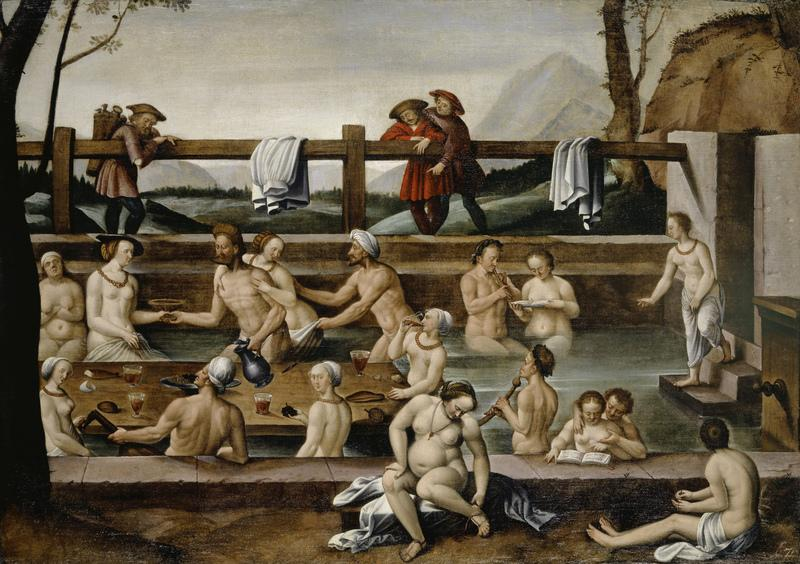
\includegraphics[width=0.8\textwidth,height=0.8\textheight]{media/image10.jpg}

}

\caption{\label{fig-bad-zu-leuk}Das Bad zu Leuk}

\end{figure}%

\begin{longtable}[]{@{}
  >{\raggedright\arraybackslash}p{(\columnwidth - 2\tabcolsep) * \real{0.0100}}
  >{\raggedright\arraybackslash}p{(\columnwidth - 2\tabcolsep) * \real{0.9900}}@{}}
\caption{Metadaten des Bildes ``Das Bad zu
Leuk''}\label{tbl-metadaten-das-bad-zu-leuk}\tabularnewline
\toprule\noalign{}
\begin{minipage}[b]{\linewidth}\raggedright
Feldname
\end{minipage} & \begin{minipage}[b]{\linewidth}\raggedright
Wert
\end{minipage} \\
\midrule\noalign{}
\endfirsthead
\toprule\noalign{}
\begin{minipage}[b]{\linewidth}\raggedright
Feldname
\end{minipage} & \begin{minipage}[b]{\linewidth}\raggedright
Wert
\end{minipage} \\
\midrule\noalign{}
\endhead
\bottomrule\noalign{}
\endlastfoot
MediaId & m123456 \\
Title & Das Bad zu Leuk \\
Subject & Kunst, Sexismus, Sexualität, sexuelle Belästigung,
Gesellschaft, Körper, Intimität, Erotik \\
Description & Das Genrebild von
\href{https://hls-dhs-dss.ch/de/articles/019088/2002-11-07/}{Hans Bock}
zeigt eine Gruppe von Menschen, die ein
\href{https://hls-dhs-dss.ch/de/articles/016308/2017-05-04/\#HVondenAnfE4ngenbisindiefrFCheNeuzeit}{Bad}
nehmen, ein beliebter Zeitvertreib im 16. Jahrhundert. Neben den
hygienischen Vorteilen bot das Bad auch Gelegenheit zur Erholung und
Geselligkeit. Für die Posen seiner Figuren verwendete Bock Vorbilder aus
anderen Werken. So war die am Beckenrand sitzende Frau bereits in seinem
\href{https://stadtgeschichtebasel.ch/blog/1000-jahre-10-geschichten-skandal-goetzendienst-und-bilderstreit-im-basler-muenster}{Venustanz}
zu sehen. Der Stil des Gemäldes erinnert an Lucas Cranachs Jungbrunnen,
der den mittelalterlichen Glauben widerspiegelt, dass bestimmte Bäder
heilen oder verjüngen können. Es ist zu erwähnen, dass beide Gemälde die
Geschlechternormen der Zeit widerspiegeln. Darüber hinaus wurden Frauen
im 16. Jahrhundert oft objektiviert und als kindlich und unschuldig
stereotypisiert, was sich in der Darstellung junger, unverhüllter Körper
in der Kunst widerspiegelt. \\
Creator & Hans Bock d.~Ä.
\href{https://www.wikidata.org/wiki/Q693916}{Q693916} \\
Publisher & Städelmuseum Frankfurt
\href{https://www.wikidata.org/wiki/Q163804}{Q163804} \\
Date & 1579 \\
Temporal & Mittelalter \\
Type & Image \\
Format & image/jpeg \\
Extent & 6676 x 4704 \\
Source & Städelmuseum Inv. 2233 \\
Language & \\
Relation & \url{https://www.staedelmuseum.de/go/ds/2233} \\
Rights & Bilddaten gemeinfrei - Kunstmuseum BaselKMB, Inv. 87 \\
License & \url{https://creativecommons.org/publicdomain/mark/1.0/} \\
\end{longtable}

\subsection{Plakat zur Völkerschau in Basel,
1926}\label{sec-plakat-zur-voelkerschau}

\begin{figure}

\centering{

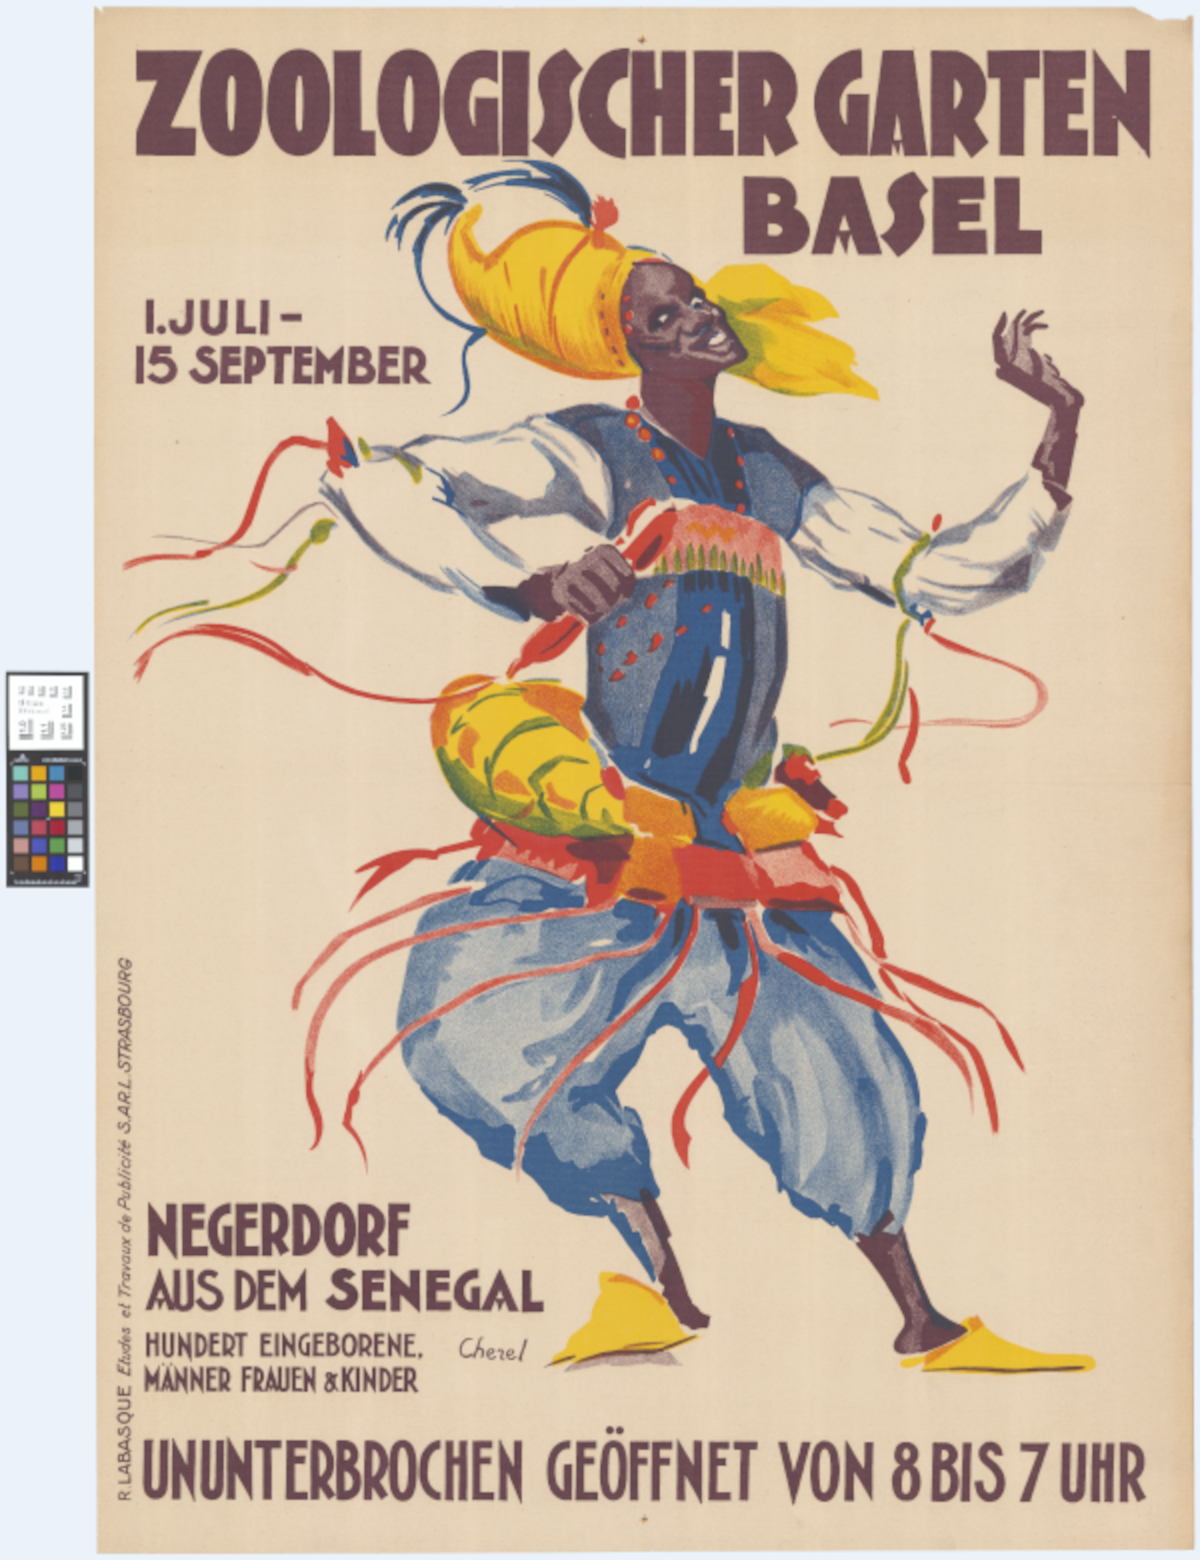
\includegraphics[width=0.8\textwidth,height=0.8\textheight]{media/image4.png}

}

\caption{\label{fig-plakat-zu-voelkerschau-in-basel-1926}Plakat zur
Völkerschau in Basel, 1926}

\end{figure}%

\begin{longtable}[]{@{}
  >{\raggedright\arraybackslash}p{(\columnwidth - 2\tabcolsep) * \real{0.0059}}
  >{\raggedright\arraybackslash}p{(\columnwidth - 2\tabcolsep) * \real{0.9941}}@{}}
\caption{Metadaten des Plakats zur Völkerschau in Basel,
1926}\label{tbl-metadaten-plakat-zur-voelkerschau-in-basel-1926}\tabularnewline
\toprule\noalign{}
\begin{minipage}[b]{\linewidth}\raggedright
Feldname
\end{minipage} & \begin{minipage}[b]{\linewidth}\raggedright
Wert
\end{minipage} \\
\midrule\noalign{}
\endfirsthead
\toprule\noalign{}
\begin{minipage}[b]{\linewidth}\raggedright
Feldname
\end{minipage} & \begin{minipage}[b]{\linewidth}\raggedright
Wert
\end{minipage} \\
\midrule\noalign{}
\endhead
\bottomrule\noalign{}
\endlastfoot
MediaId & m123457 \\
Title & Plakat zur Völkerschau in Basel, 1926 \\
Subject & Kolonialismus, Imperialismus, Rassismus, Öffentlichkeit,
Kultur \\
Description & Im Zeitraum zwischen 1879 und 1935 fanden im Basler Zoo 21
sogenannte
``\href{https://www.baslerstadtbuch.ch/stadtbuch/1992/1992_2247.html}{Völkerschauen''
(Achtung Link führt zu diskriminierenden Bildern)} - heute auch
Menschenzoos genannt - statt, in denen Menschen aus verschiedenen
Kulturen \emph{ausgestellt} wurden. Schweizweit fanden solche Schauen
bis ins Jahr 1964 statt. Bei diesen Veranstaltungen wurden Menschen
entweder in festen Einrichtungen, mobilen Zoos oder sogar in
Zirkusvorführungen zur Schau gestellt. Dahinter stand ein rassistisches,
imperialistisches und kolonialistische\emph{s} Menschenbild. Die in den
Werbeplakaten verwendete Bildsprache bediente sich an kolonialen
Fantasien der europäischen Bevölkerung und stellte die Menschen als
vermeintlich''primitiv''\emph{,} ``wild'', ``kriegerisch'' und
``exotisch'' dar, was zu einer Aufrechterhaltung von negativen
Stereotypen führte. Die Schauen waren in der Ideologie der
``Rassentheorie'' verwurzelt, die eine Überlegenheit der europäischen
Bevölkerung gegenüber anderen Kulturen auf angeblich wissenschaftlicher
Grundlage behauptete. Die Ideologie der
\href{https://hls-dhs-dss.ch/de/articles/060537/2024-04-08/}{Rassentheorie}
wurde genutzt, um die Ausstellung dieser Menschen als akzeptabel
darzustellen, indem sie als blosse Objekte zur Unterhaltung des
Publikums behandelt wurden. Die tief verwurzelten Stereotypen und
Vorurteile wurden über Generationen hinweg in
\href{https://mirsindvoda.ch/voelkerschauen-in-der-schweiz/}{Kultur und
Sprache} weitergegeben, sei es durch Bücher, Filme oder
Erzählungen.Einige der Bilder, welche einst dazu gedient haben sollen,
die Unterdrückung oder vermeintliche "Rettung" und den "Schutz vor sich
selbst" bestimmter "primitiver und unzivilisierter Völker" zu
rechtfertigen, bestehen teilweise noch bis heute und manifestieren sich
in unterschiedlichen Formen von Diskriminierung. \\
Creator & \\
Publisher &
StaBS~\href{https://www.wikidata.org/wiki/Q2324698}{Q2324698} \\
Date & 1926 \\
Temporal & Zeitgeschichte \\
Type & Image \\
Format & image/tiff \\
Extent & 23376 x 30371 \\
Source & StaBs BSL 1001 N 7 \\
Language &
\href{https://www.loc.gov/standards/iso639-2/php/langcodes_name.php?code_ID=160}{deu} \\
Relation & \url{https://dls.staatsarchiv.bs.ch/records/135592} \\
Rights & print und print digital (2022-)Staatsarchiv Basel-Stadt, BSL
1001 N 7 \\
License & \url{https://creativecommons.org/publicdomain/mark/1.0/} \\
\end{longtable}

\subsection{Schnitzerei am Chorgestühl des Basler
Münsters}\label{schnitzerei-am-chorgestuxfchl-des-basler-muxfcnsters}

\begin{figure}

\centering{

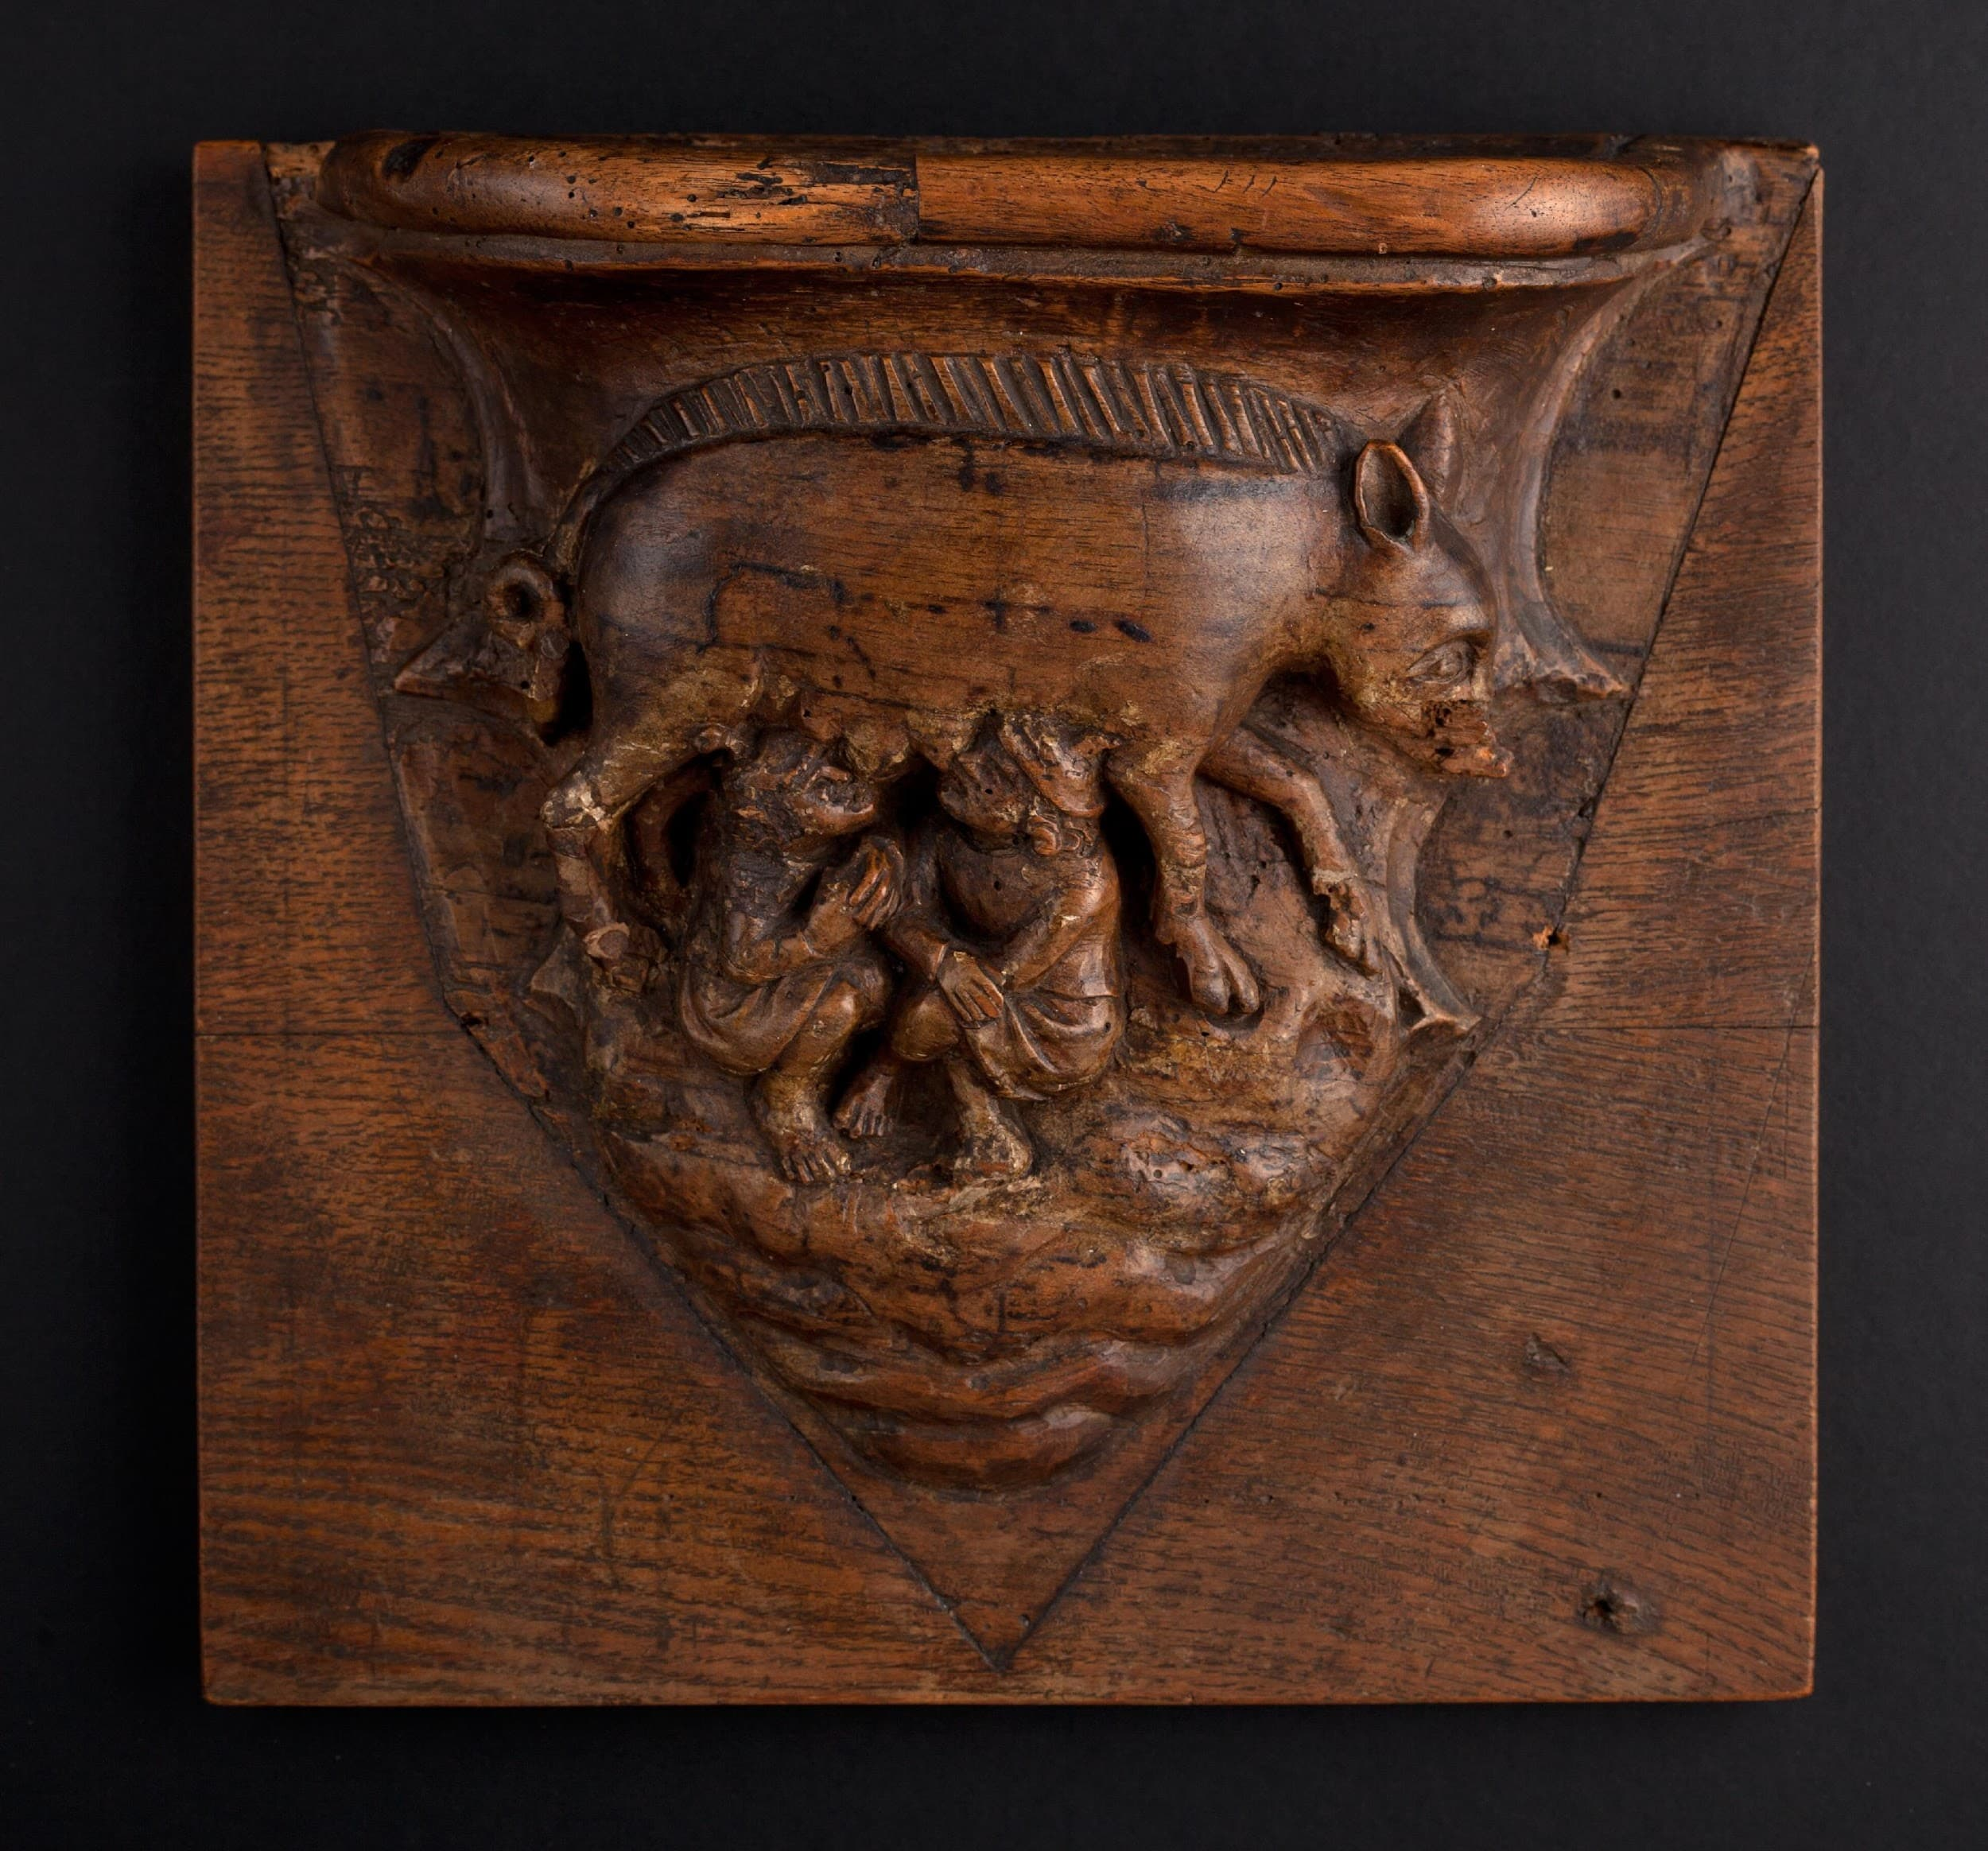
\includegraphics[width=0.8\textwidth,height=0.8\textheight]{media/image12.jpg}

}

\caption{\label{fig-schnitzerei-am-chorgestuehl-des-basler-muensters}Schnitzerei
am Chorgestühl des Basler Münsters}

\end{figure}%

\begin{longtable}[]{@{}
  >{\raggedright\arraybackslash}p{(\columnwidth - 2\tabcolsep) * \real{0.0101}}
  >{\raggedright\arraybackslash}p{(\columnwidth - 2\tabcolsep) * \real{0.9899}}@{}}
\caption{Metadaten der Schnitzerei am Chorgestühl des Basler
Münsters}\label{tbl-metadaten-schnitzerei-am-chorgestuehl-des-basler-muensters}\tabularnewline
\toprule\noalign{}
\begin{minipage}[b]{\linewidth}\raggedright
Feldname
\end{minipage} & \begin{minipage}[b]{\linewidth}\raggedright
Wert
\end{minipage} \\
\midrule\noalign{}
\endfirsthead
\toprule\noalign{}
\begin{minipage}[b]{\linewidth}\raggedright
Feldname
\end{minipage} & \begin{minipage}[b]{\linewidth}\raggedright
Wert
\end{minipage} \\
\midrule\noalign{}
\endhead
\bottomrule\noalign{}
\endlastfoot
MediaId & m123458 \\
Title & Schnitzerei am Chorgestühl des Basler Münsters \\
Subject & Antisemitismus, Judentum, Kunst, Religion, Kirche \\
Description & Ein Schnitzwerk im Chorgestühl des Basler Münsters aus der
Zeit um 1380 zeigt eine beleidigende Darstellung von jüdischen Personen.
Das Bild zeigt zwei Personen, die Milch direkt von einer Sau trinken,
was eine Karikatur des jüdischen Nahrungstabus für Schweine ist.
Ausserdem symbolisierten Schweine im Mittelalter Sünde und Unreine sowie
in der christlichen Ikonographie steht das Schwein sinnbildlich für den
Teufel. Die jüdischen Personen werden
\href{https://www.gra.ch/bildung/glossar/judensau/}{im Chorgestühl} in
der damals gesetzlich vorgeschriebenen Kleidung dargestellt. So tragen
die Personen spitze Hüte. Die Darstellungen zeugen von religiösen sowie
kulturellen Vorstellungen, jüdische Personen zu diskriminieren und
gesellschaftlich auszuschliessen. In Europa gab es mindestens 50 solcher
Darstellungen, die auch in oder an Rathäusern angebracht waren. Einige
bestehen noch heute. Das Original der Schnitzerei im Basler Münster
wurde aus ungeklärten Gründen zerstört. Die Replika wurde erst im Jahr
1996 entfernt und befindet sich nun im Jüdischen Museum der Schweiz. \\
Creator & \\
Publisher & Denkmalpflege Basel Stadt
\href{https://www.wikidata.org/wiki/Q27479725}{Q27479725} \\
Date & 1384/1390 \\
Temporal & Mittelalter \\
Type & Image \\
Format & image/tiff \\
Extent & 3887 x 3619 \\
Source & Sammlung Münsterfoto \\
Language & \\
Relation & \\
Rights & In CopyrightKantonale Denkmalpflege Basel-Stadt, Foto Hans
Grunert \\
License & \url{http://rightsstatements.org/vocab/InC-RUU/1.0/} \\
\end{longtable}

\subsection{Hie Basel Hie Schweizer Boden - Liste
3}\label{hie-basel-hie-schweizer-boden---liste-3}

\begin{figure}

\centering{

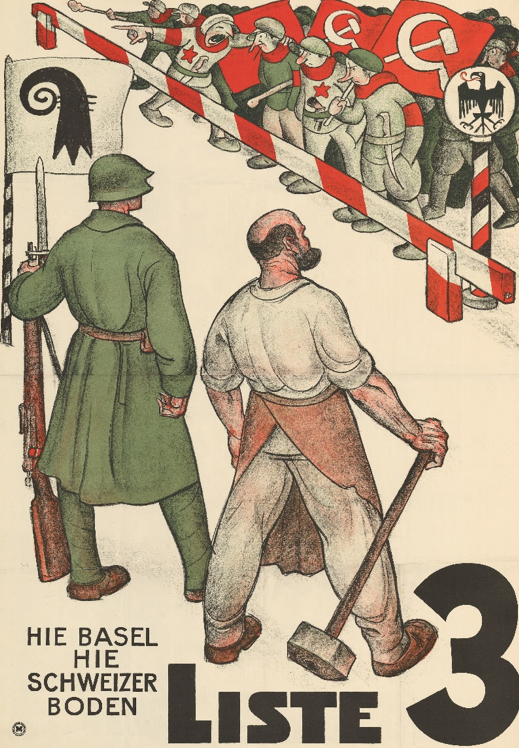
\includegraphics[width=0.8\textwidth,height=0.8\textheight]{media/image6.png}

}

\caption{\label{fig-hie-basel-hie-schweizer-boden-liste-3}Hie Basel Hie
Schweizer Boden - Liste 3}

\end{figure}%

\begin{longtable}[]{@{}
  >{\raggedright\arraybackslash}p{(\columnwidth - 2\tabcolsep) * \real{0.0156}}
  >{\raggedright\arraybackslash}p{(\columnwidth - 2\tabcolsep) * \real{0.9844}}@{}}
\caption{Metadaten des Plakats ``Hie Basel Hie Schweizer Boden - Liste
3''}\label{tbl-metadaten-hie-basel-hie-schweizer-boden-liste-3}\tabularnewline
\toprule\noalign{}
\begin{minipage}[b]{\linewidth}\raggedright
Feldname
\end{minipage} & \begin{minipage}[b]{\linewidth}\raggedright
Wert
\end{minipage} \\
\midrule\noalign{}
\endfirsthead
\toprule\noalign{}
\begin{minipage}[b]{\linewidth}\raggedright
Feldname
\end{minipage} & \begin{minipage}[b]{\linewidth}\raggedright
Wert
\end{minipage} \\
\midrule\noalign{}
\endhead
\bottomrule\noalign{}
\endlastfoot
MediaId & m123459 \\
Title & Hie Basel Hie Schweizer Boden - Liste 3 \\
Subject & Politik, Rassismus, Diskurs, Nationalismus, Nationalstaat,
Sozialismus, Werbung \\
Description & Das undatierte Wahlplakat der Bürger- und Gewerbepartei
(BGP), das von
\href{https://hls-dhs-dss.ch/de/articles/048316/2010-09-28/}{Otto
Plattner} erstellt wurde, spiegelt die ideologischen Auswirkungen des
\href{https://www.baslerstadtbuch.ch/chronik/1919/08/01/am-donnerstag-31-juli-brach-in-basel-ein-generalstreik-aus.html}{Generalstreiks}
wider. Die bürgerliche Partei versuchte, dem Aufstieg der
Kommunistischen Partei (KP) entschieden entgegenzutreten und nutzte
dabei rassistische Darstellungen: Auf dem Plakat wird das
Schreckgespenst des Kommunismus als eine gewalttätige Menschenmenge mit
überzeichneten Nasen dargestellt, die als Bedrohung für die Schweiz und
ihre Bürger*innen angesehen wird. \\
Creator & Otto Plattner
\href{https://www.wikidata.org/wiki/Q1748710}{Q1748710} \\
Publisher & Plakatsammlung, Schule für Gestaltung
\href{https://www.wikidata.org/wiki/Q19362827}{Q19362827} \\
Date & 1925\textasciitilde{} \\
Temporal & Zeitgeschichte \\
Type & Image \\
Format & image/tiff \\
Extent & 2877 x 4096 \\
Source & CH-000957-X:4432 \\
Language &
\href{https://www.loc.gov/standards/iso639-2/php/langcodes_name.php?code_ID=177}{gsw} \\
Relation &
\url{https://commons.wikimedia.org/wiki/File:CH-000957-X-4432_Plattner.tif}\url{https://www.recherche-plakatsammlungbasel.ch/objects/49187/hie-basel-hie-schweizer-boden-liste-3?ctx=b34b16b1c3a4902bd2474a31359b3c34bb330ced&idx=37} \\
Rights & Public Domain \\
License & \url{https://creativecommons.org/publicdomain/mark/1.0/} \\
\end{longtable}

\subsection{Zeitungsinserat in der National-Zeitung,
1955}\label{zeitungsinserat-in-der-national-zeitung-1955}

\begin{figure}

\centering{

\includegraphics[width=0.8\textwidth,height=0.8\textheight]{media/image11.png}

}

\caption{\label{fig-zeitungsinserat-in-der-national-zeitung-1955}Zeitungsinserat
in der National-Zeitung, 1955}

\end{figure}%

\begin{longtable}[]{@{}
  >{\raggedright\arraybackslash}p{(\columnwidth - 2\tabcolsep) * \real{0.0125}}
  >{\raggedright\arraybackslash}p{(\columnwidth - 2\tabcolsep) * \real{0.9875}}@{}}
\caption{Metadaten des Zeitungsinserats in der National-Zeitung,
1955}\label{tbl-metadaten-zeitungsinserat-in-der-national-zeitung-1955}\tabularnewline
\toprule\noalign{}
\begin{minipage}[b]{\linewidth}\raggedright
Feldname
\end{minipage} & \begin{minipage}[b]{\linewidth}\raggedright
Wert
\end{minipage} \\
\midrule\noalign{}
\endfirsthead
\toprule\noalign{}
\begin{minipage}[b]{\linewidth}\raggedright
Feldname
\end{minipage} & \begin{minipage}[b]{\linewidth}\raggedright
Wert
\end{minipage} \\
\midrule\noalign{}
\endhead
\bottomrule\noalign{}
\endlastfoot
MediaId & m123410 \\
Title & Zeitungsinserat in der National-Zeitung, 1955 \\
Subject & Bildung, Biologismus, Rassismus, Ableismus, Ehe, Patriarchat,
Sexismus, Sexualität, Familie, Familienbild, Familienform, Presse \\
Description & Seit 1933 wurde eine Ehe- und Sexualberatungsstelle vom
Gesundheitsamt Basel-Stadt eingerichtet. Neben individuellen
Sprechstunden wurden auch Ehekurse für Verlobte und Neuverheiratete
angeboten. In diesen Kursen wurden die Teilnehmenden in Bereichen wie
Medizin, Hygiene, Psychologie und Recht geschult. Die Gründung der
Beratungsstelle hatte eugenische Motive. Die Absicht bestand darin,
nicht nur über Verhütung aufzuklären, sondern auch Eheanwärter*innen~in
zeitgenössischer Vererbungslehre zu informieren. Solche eugenischen
Ansätze gingen auch von leitenden Ärzten der Basler Psychiatrie aus. Sie
beeinflussten auch die gesetzlichen Bestimmungen des Schweizerischen
Zivilgesetzbuches über die Eheschliessung von "Geisteskranken" und die
Appelle in der Eheberatung, insbesondere zu Themen wie Sterilisation,
Abtreibung, Einbürgerung, Ausweisung und Rückführung. \\
Creator & Gesundheitsamt Basel-Stadt
\href{https://www.wikidata.org/wiki/Q33121140}{Q33121140} \\
Publisher &
StaBS~\href{https://www.wikidata.org/wiki/Q2324698}{Q2324698} \\
Date & 1955 \\
Temporal & Zeitgeschichte \\
Type & Text \\
Format & image/tiff \\
Extent & 7508 x 7785 \\
Source & StaBS, SD-REG 5a 0.21.0 (1) 2 \\
Language &
\href{https://www.loc.gov/standards/iso639-2/php/langcodes_name.php?code_ID=160}{deu} \\
Relation & \url{https://dls.staatsarchiv.bs.ch/records/373373} \\
Rights & In CopyrightStABS, SD-REG 5a 0.21.0 (1) 2 \\
License & \url{http://rightsstatements.org/vocab/InC/1.0/} \\
\end{longtable}

\subsection{Die ausländische Wohnbevölkerung von Basel-Stadt nach
Heimatnation,
1920--1965}\label{die-ausluxe4ndische-wohnbevuxf6lkerung-von-basel-stadt-nach-heimatnation-19201965}

\begin{figure}

\centering{

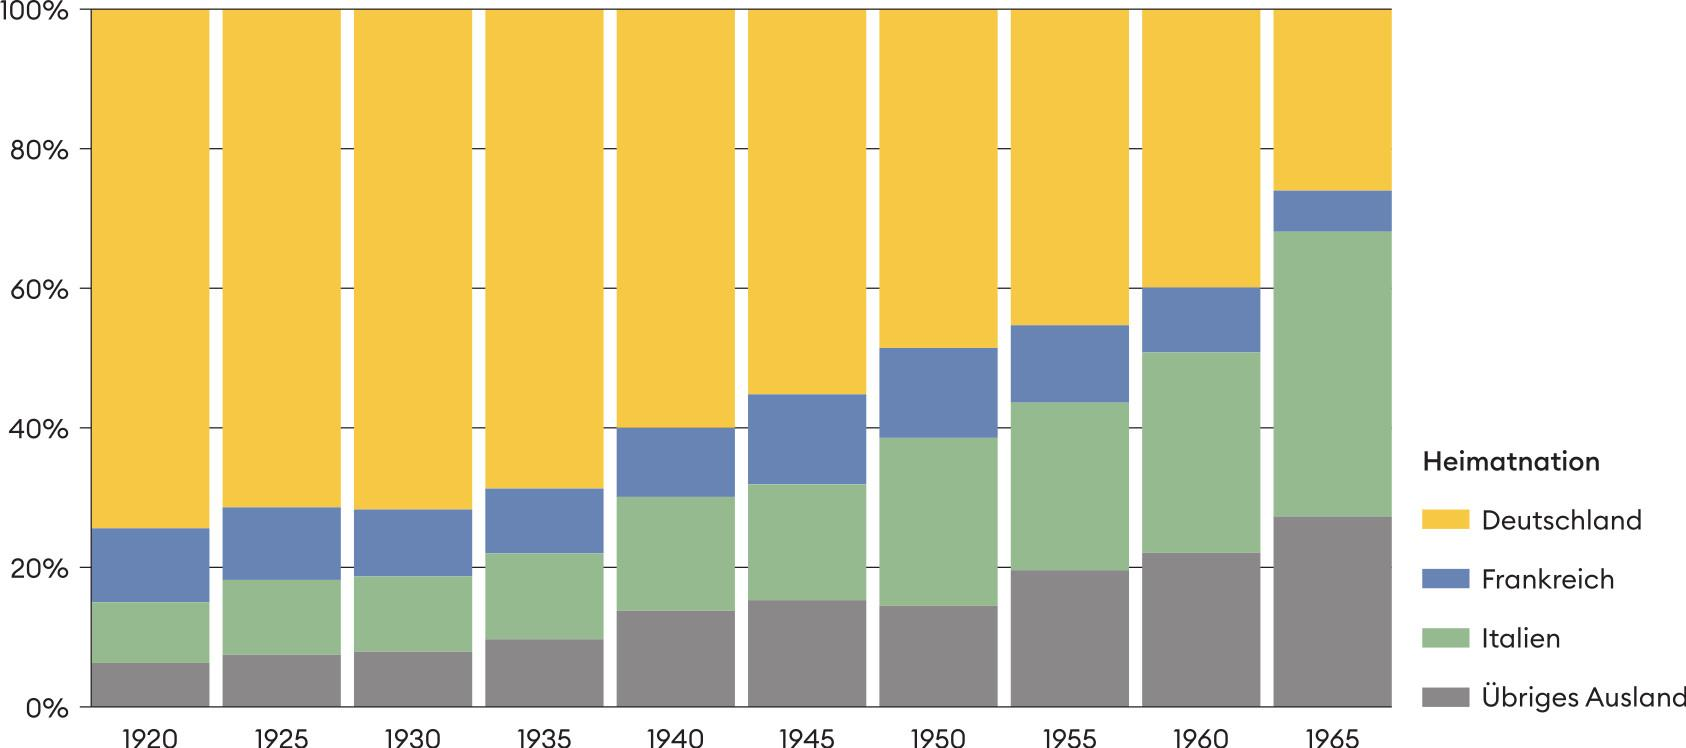
\includegraphics[width=0.8\textwidth,height=0.8\textheight]{media/image14.jpg}

}

\caption{\label{fig-die-auslaendische-wohnbevoelkerung-von-basel-stadt-nach-heimatnation-1920-1965}Die
ausländische Wohnbevölkerung von Basel-Stadt nach Heimatnation,
1920--1965}

\end{figure}%

\begin{longtable}[]{@{}
  >{\raggedright\arraybackslash}p{(\columnwidth - 2\tabcolsep) * \real{0.0060}}
  >{\raggedright\arraybackslash}p{(\columnwidth - 2\tabcolsep) * \real{0.9940}}@{}}
\caption{Metadaten der Statistik ``Die ausländische Wohnbevölkerung von
Basel-Stadt nach Heimatnation,
1920--1965''}\label{tbl-metadaten-die-auslaendische-wohnbevoelkerung-von-basel-stadt-nach-heimatnation-1920-1965}\tabularnewline
\toprule\noalign{}
\begin{minipage}[b]{\linewidth}\raggedright
Feldname
\end{minipage} & \begin{minipage}[b]{\linewidth}\raggedright
Wert
\end{minipage} \\
\midrule\noalign{}
\endfirsthead
\toprule\noalign{}
\begin{minipage}[b]{\linewidth}\raggedright
Feldname
\end{minipage} & \begin{minipage}[b]{\linewidth}\raggedright
Wert
\end{minipage} \\
\midrule\noalign{}
\endhead
\bottomrule\noalign{}
\endlastfoot
MediaId & m123411 \\
Title & Die ausländische Wohnbevölkerung von Basel-Stadt nach
Heimatnation, 1920--1965 \\
Subject & Asyl, Migration, Minderheit, Integration, Heimat,
Gesellschaft, Gesetz \\
Description & Die vorliegende Statistik bietet Informationen über die
Verteilung von deutscher, französischer oder italienischer
Staatsbürgerschaft im Kanton Basel-Stadt im Zeitraum von 1920 bis 1965.
Der grau schraffierte Bereich repräsentiert die übrigen
Nationalitäten.Aus der Statistik lassen sich zwei signifikante Trends
ablesen: Der Anteil der Personen deutscher Nationalität nahm
kontinuierlich ab. Dies ist auf verschiedene Faktoren zurückzuführen,
unter anderem auf die Ablehnung von Personen deutscher Nationalität, die
bereits seit Jahrzehnten in der Schweiz lebten, nach dem Zweiten
Weltkrieg. Die Gründe für die Ablehnung der Gesuche waren vielfältig und
umfassten unter anderem Sympathien für den Nationalsozialismus sowie das
Argument, dass diese Personen als zu wenig "schweizerisch" angesehen
wurden.Auf der anderen Seite stieg der Anteil der Personen aus Italien
in den 1960er Jahren deutlich an. Es ist anzumerken, dass der Anteil
sogar noch höher gewesen wäre, wenn die Gastarbeiter*innen aus anderen
Kantonen, die zu diesem Zeitpunkt in der Region tätig waren, in dieser
Statistik mit einbezogen worden wären. Ausserdem fanden die
Volkszählungen im Dezember statt und daher sind saisonale
Gastarbeiter*innen nicht konsistent erfasst.Es ist bekannt, dass die
Basler Regierung die schweizweite Politik der Arbeitsmigration, die auch
als "Fremdarbeit" bekannt ist, unterstützte. Es ist wichtig anzumerken,
dass die Umsetzung dieser Politik damals auf bestimmten Arbeitsmodellen
(\href{https://hls-dhs-dss.ch/de/articles/007991/2006-12-07/}{Rotationsprinzip})
basierte, die heute als problematisch angesehen werden. Integration in
die Basler Gesellschaft wurde nicht ausreichend gefördert und
italienische Arbeiter*innen wurden oft dazu angehalten, die Stadt nach
neun Monaten wieder zu verlassen. \\
Creator & Stadt.Geschichte.Basel
\href{https://www.wikidata.org/wiki/Q122442230}{Q122442230} \\
Publisher & Stadt.Geschichte.Basel
\href{https://www.wikidata.org/wiki/Q122442230}{Q122442230} \\
Date & 1920/1965 \\
Temporal & Zeitgeschichte \\
Type & Image \\
Format & image/jpeg \\
Extent & 1686 x 748 \\
Source & JB 1941, S. 24 / JB 1951, S. 25 / JB 1966, S. 32 \\
Language &
\href{https://www.loc.gov/standards/iso639-2/php/langcodes_name.php?code_ID=160}{deu} \\
Relation & \\
Rights & Public DomainQuelle: JB 1941, S. 24 / JB 1951, S. 25 / JB 1966,
S. 32. Bearbeitung: Nico Görlich / Moritz Twente \\
License & \url{https://creativecommons.org/publicdomain/mark/1.0/} \\
\end{longtable}

\subsection{Basler Brandmarkeisen, 17.
Jahrhundert}\label{basler-brandmarkeisen-17.-jahrhundert}

\begin{figure}

\centering{

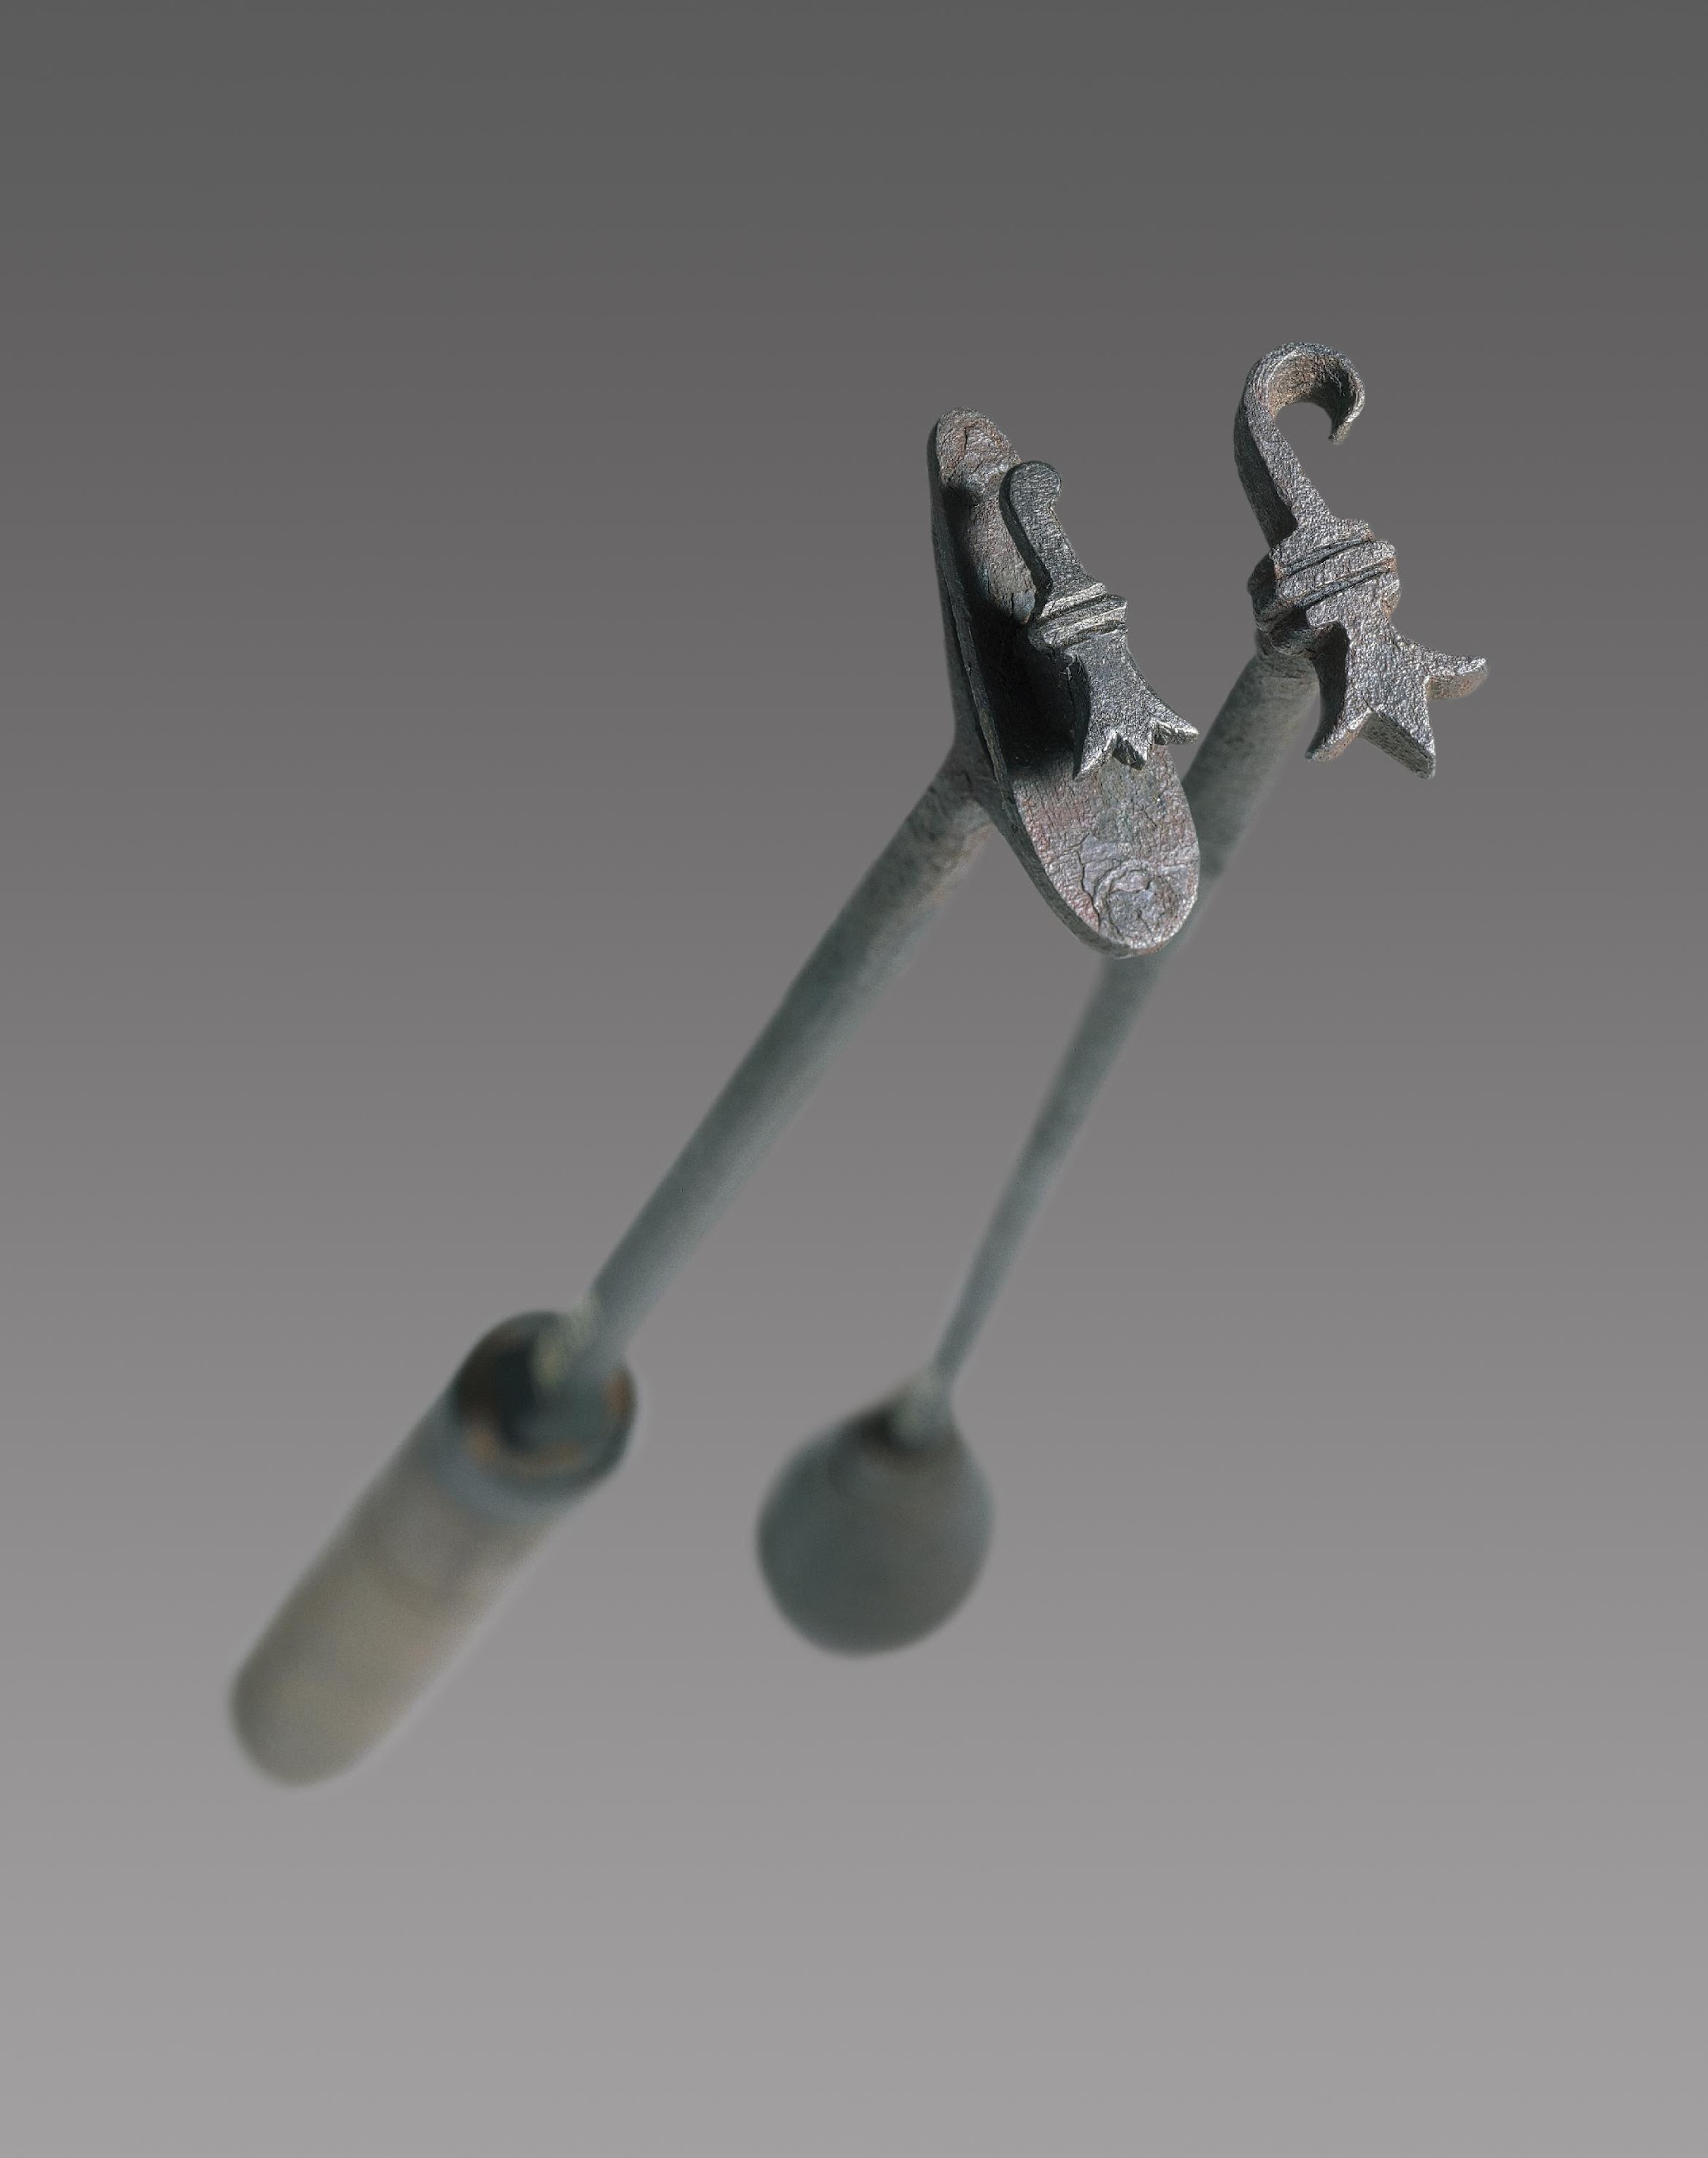
\includegraphics[width=0.8\textwidth,height=0.8\textheight]{media/image13.jpg}

}

\caption{\label{fig-basler-brandmarkeisen-17-jahrhundert}Basler
Brandmarkeisen, 17. Jahrhundert}

\end{figure}%

\begin{longtable}[]{@{}
  >{\raggedright\arraybackslash}p{(\columnwidth - 2\tabcolsep) * \real{0.0182}}
  >{\raggedright\arraybackslash}p{(\columnwidth - 2\tabcolsep) * \real{0.9818}}@{}}
\caption{Metadaten der Basler Brandmarkeisen, 17.
Jahrhundert}\label{tbl-metadaten-basler-brandmarkeisen-17-jahrhundert}\tabularnewline
\toprule\noalign{}
\begin{minipage}[b]{\linewidth}\raggedright
Feldname
\end{minipage} & \begin{minipage}[b]{\linewidth}\raggedright
Wert
\end{minipage} \\
\midrule\noalign{}
\endfirsthead
\toprule\noalign{}
\begin{minipage}[b]{\linewidth}\raggedright
Feldname
\end{minipage} & \begin{minipage}[b]{\linewidth}\raggedright
Wert
\end{minipage} \\
\midrule\noalign{}
\endhead
\bottomrule\noalign{}
\endlastfoot
MediaId & m123412 \\
Title & Basler Brandmarkeisen, 17. Jahrhundert \\
Subject & Geschichte, Integration, Stadt, Stigmatisierung, Gewalt,
Körper, Kriminalität, Misshandlung, Täter, Täterin \\
Description & Der Basler Rat verwendete unterschiedliche Methoden, um
Straftaten zu bestrafen. Ein solches Instrument war das Basler Wappen,
das zwei Bedeutungen hatte: Integration und Verbannung. Der Rat liess
Verbrecher*innen mit einem Brandeisen brandmarken, um ihre Verbannung
aus Basel sichtbar zu machen. Diese Strafe gehörte zu den sogenannten
Schand- und Ehrenstrafen. Das Ziel war es, die Schuldigen öffentlich
blosszustellen und zu erniedrigen. Die Brandmarkung war dauerhaft
sichtbar und hatte daher im Gegensatz zu Strafen wie dem Pranger
weitreichende Konsequenzen für die betroffenen Personen. \\
Creator & \\
Publisher & Historisches Museum Basel
\href{http://www.wikidata.org/entity/Q386286}{Q386286} \\
Date & 1600/1700 \\
Temporal & Neuzeit \\
Type & Image \\
Format & image/jpeg \\
Extent & 3416 x 4315 \\
Source & HMB, Inv. 1921.1258. und 1921.1259. \\
Language & \\
Relation &
\url{https://www.hmb.ch/museen/sammlungsobjekte/einzelansicht/s/brandmarkeisen/} \\
Rights & CC BY-SA 4.0, Peter PortnerHMB, Inv. 1921.1258 + 1259, Foto
Peter Portner \\
License & \url{https://creativecommons.org/licenses/by-sa/4.0/} \\
\end{longtable}

\subsection{Plan mit Verteilung jüdischer
Häuser}\label{plan-mit-verteilung-juxfcdischer-huxe4user}

\begin{figure}

\centering{

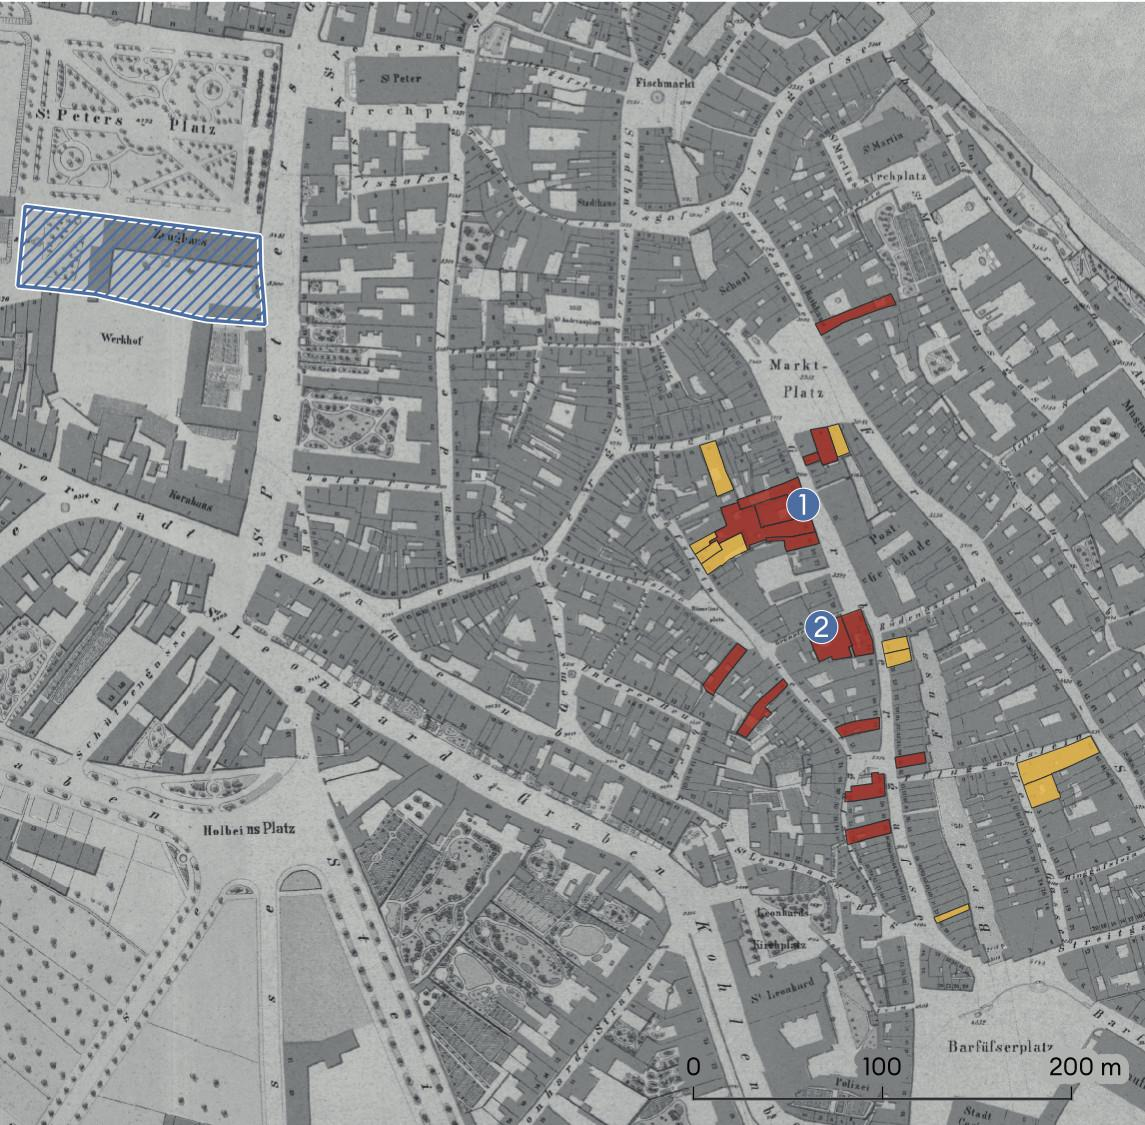
\includegraphics[width=0.8\textwidth,height=0.8\textheight]{media/image15.jpg}

}

\caption{\label{fig-plan-mit-verteilung-juedischer-haeuser}Plan mit
Verteilung jüdischer Häuser}

\end{figure}%

\begin{longtable}[]{@{}
  >{\raggedright\arraybackslash}p{(\columnwidth - 2\tabcolsep) * \real{0.0119}}
  >{\raggedright\arraybackslash}p{(\columnwidth - 2\tabcolsep) * \real{0.9881}}@{}}
\caption{Metadaten des Plans mit Verteilung jüdischer
Häuser}\label{tbl-metadaten-plan-mit-verteilung-juedischer-haeuser}\tabularnewline
\toprule\noalign{}
\begin{minipage}[b]{\linewidth}\raggedright
Feldname
\end{minipage} & \begin{minipage}[b]{\linewidth}\raggedright
Wert
\end{minipage} \\
\midrule\noalign{}
\endfirsthead
\toprule\noalign{}
\begin{minipage}[b]{\linewidth}\raggedright
Feldname
\end{minipage} & \begin{minipage}[b]{\linewidth}\raggedright
Wert
\end{minipage} \\
\midrule\noalign{}
\endhead
\bottomrule\noalign{}
\endlastfoot
MediaId & m123413 \\
Title & Plan mit Verteilung jüdischer Häuser \\
Subject & Antisemitismus, Judentum, Gesellschaft, Wohnen, Stadt \\
Description & Die Karte zeigt die Verteilung von jüdischen Häusern,
Gemeinden, Synagogen sowie Friedhöfen im mittelalterlichen Basel. Die
erste
\href{https://eterna.unibas.ch/bodenforschungmh/article/view/1163}{jüdische
Gemeinde} ist auf den Zeitraum von 1200 bis Anfang 1349 datiert und die
zweite Gemeinde von 1362 bis 1397. Beide Gemeinden besassen eine
Synagoge und einen Friedhof. Am 16. Januar 1349 wurde die erste Gemeinde
vernichtet. Im Zusammenhang der Pestepidemie wurde die jüdische
Gemeinschaft der angeblichen "Brunnenvergiftung" bezichtigt und deshalb
auf der Rheininsel bei Basel ermordet. Solche Anklagen und
anschliessende Ermordungen fanden zu dieser Zeit nicht nur in Basel
statt. Ab 1362 siedelten sich wieder vermehrt jüdische Familien in Basel
an. Der Standort der Synagoge hatte sich wohl aufgrund Beschlagnahmung
und Enteignung der Synagoge der ersten Gemeinde verschoben. Sie lag nun
in der Grünpfahlgasse.~ \\
Creator & Stadt.Geschichte.Basel
\href{https://www.wikidata.org/wiki/Q122442230}{Q122442230} \\
Publisher & Stadt.Geschichte.Basel
\href{https://www.wikidata.org/wiki/Q122442230}{Q122442230} \\
Date & 1398 \\
Temporal & Mittelalter \\
Type & Image \\
Format & image/jpeg \\
Extent & 1145 x 1125 / 495 x 329 \\
Source & Alder/Matt 2010, S. 28 \\
Language &
\href{https://www.loc.gov/standards/iso639-2/php/langcodes_name.php?code_ID=160}{deu} \\
Relation & \\
Rights & Public DomainQuelle: Alder/Matt 2010, S. 28. Bearbeitung: Nico
Görlich / Moritz Twente \\
License & \url{https://creativecommons.org/publicdomain/mark/1.0/} \\
\end{longtable}

\subsection{Lebensbilder}\label{lebensbilder}

Für den ersten Geschichtsband der Stadt.Geschichte.Basel werden unter
anderem Lebensbilder angefertigt. Lebensbilder dienen dazu, die
Lebensumstände der ur- und frühzeitlichen Menschen zu rekonstruieren.
Sie werden in diesem Handbuch ebenfalls thematisiert, da sie wie
historische Quellen Diskriminierung und Stereotypisierungen enthalten
können. So wird beispielsweise auf Lebensbildern oftmals das Bild einer
Kernfamilie dargestellt. Diese Kernfamilie entspricht dem heutigen
stereotypen Familienideal, das aus Vater, Mutter und zwei Kindern
besteht. Zudem sind Kinder auf Lebensbildern grundsätzlich
unterrepräsentiert. Diskurse zur Darstellung von sozialen Strukturen und
Verhältnissen auf Lebensbildern fanden in der Archäologie erst ab den
2000er-Jahren statt. Reflexionsprozesse sind deshalb wichtig, weil
Lebensbilder dazu beitragen, ein "Bild von Verhältnissen, die schon
immer so waren" zu festigen. Die Leser*innen betrachten die
dargestellten Stereotypen als selbstverständlich und nehmen an, dass sie
seit langem existieren und daher als richtig angesehen werden sollten,
ohne, dass die Bilder infrage gestellt werden.

Im Folgenden werden anhand "negativer" Beispiele Stereotypen sowie
Diskriminierungen in Lebensbildern präsentiert. Im zweiten Unterkapitel
werden "positive" Beispiele gezeigt.

\subsubsection{Negative Beispiele von
Lebensbildern}\label{negative-beispiele-von-lebensbildern}

\paragraph{Androzentrismus}\label{androzentrismus}

\begin{figure}

\centering{

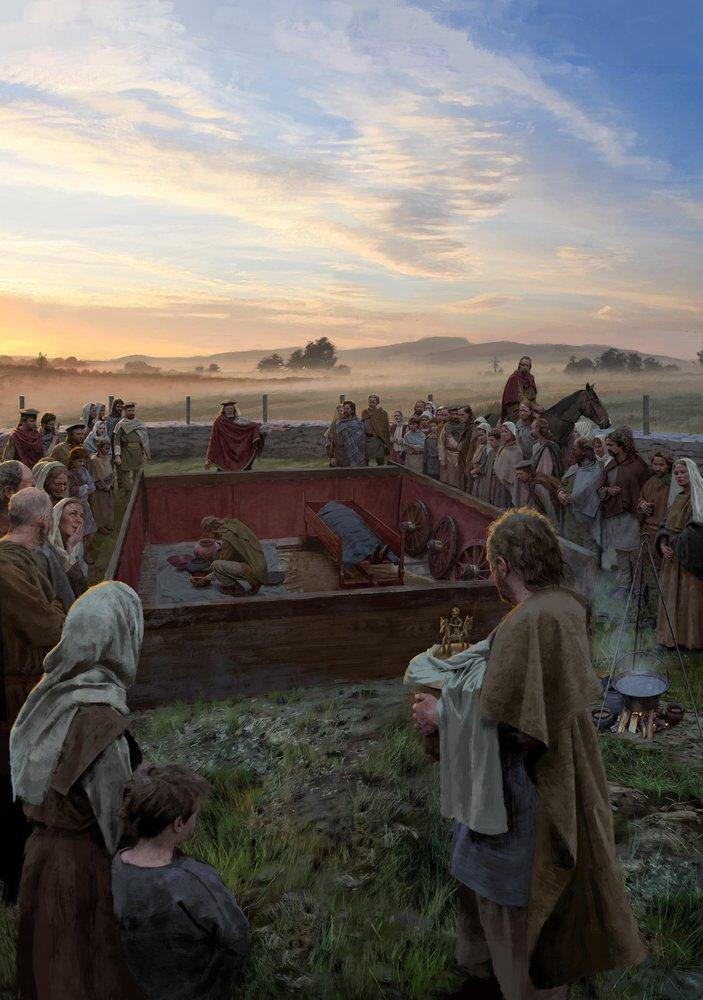
\includegraphics[width=0.8\textwidth,height=0.8\textheight]{media/image8.jpg}

}

\caption{\label{fig-bestattung-von-unlingen}Bestattung von Unlingen}

\end{figure}%

\begin{longtable}[]{@{}
  >{\raggedright\arraybackslash}p{(\columnwidth - 2\tabcolsep) * \real{0.0171}}
  >{\raggedright\arraybackslash}p{(\columnwidth - 2\tabcolsep) * \real{0.9829}}@{}}
\caption{Metadaten der Bestattung von
Unlingen}\label{tbl-metadaten-bestattung-von-unlingen}\tabularnewline
\toprule\noalign{}
\begin{minipage}[b]{\linewidth}\raggedright
Feldname
\end{minipage} & \begin{minipage}[b]{\linewidth}\raggedright
Wert
\end{minipage} \\
\midrule\noalign{}
\endfirsthead
\toprule\noalign{}
\begin{minipage}[b]{\linewidth}\raggedright
Feldname
\end{minipage} & \begin{minipage}[b]{\linewidth}\raggedright
Wert
\end{minipage} \\
\midrule\noalign{}
\endhead
\bottomrule\noalign{}
\endlastfoot
MediaId & m123414 \\
Filename & \\
Title & Bestattung von Unlingen \\
Subject & Geschlechterbild, Geschlechterstereotyp,
Geschlechterverhältnis, Tod \\
Description & Bei Unlingen am Fuss des Berges Bussen wurde im Jahr 1890
ein keltisches Grab entdeckt. Bei den Grabungen wurden drei
frühkeltische Grabhügel mit insgesamt fünf Bestattungen des 8. bis 5.
Jahrhunderts v. Chr. entdeckt. Zu diesem Grabungsfund wurde ein
Lebensbild entwickelt. Darin haben Männer eine natürliche
Vormachtstellung. Frauen sind selten bis nie in einer führenden sozialen
Rolle dargestellt. Wichtige soziale Ereignisse wie Feste und
Bestattungen werden von Männern geleitet und massgeblich begleitet.
Frauen dagegen werden als passive Beobachterinnen dargestellt, die in
der gezeigten Handlung keine aktive Rolle spielen. \\
Creator & Landesamt für Denkmalpflege im Regierungspräsidium Stuttgart
\href{https://www.wikidata.org/wiki/Q28738904}{Q28738904}, Samson
Götze \\
Publisher & Landesamt für Denkmalpflege im Regierungspräsidium Stuttgart
\href{https://www.wikidata.org/wiki/Q28738904}{Q28738904}, Samson
Götze \\
Date & \\
Era & Frühgeschichte \\
Type & Image \\
Format & image/jpeg \\
Extent & 703 x 1000 \\
Source & Landesamt für Denkmalpflege im Regierungspräsidium Stuttgart
\href{https://www.wikidata.org/wiki/Q28738904}{Q28738904}/Samson
Götze \\
Language & \\
Relation &
\url{https://www.archaeologie-an-der-oberen-donau.de/forschungsprojekte/dfg-langfristprojekt/graeber/unlingen} \\
Rights & Samson Götze \\
License &
\url{https://rightsstatements.org/page/InC-RUU/1.0/?language=de} \\
\end{longtable}

\paragraph{Rollenverteilung zwischen den
Geschlechtern}\label{rollenverteilung-zwischen-den-geschlechtern}

\begin{figure}

\centering{

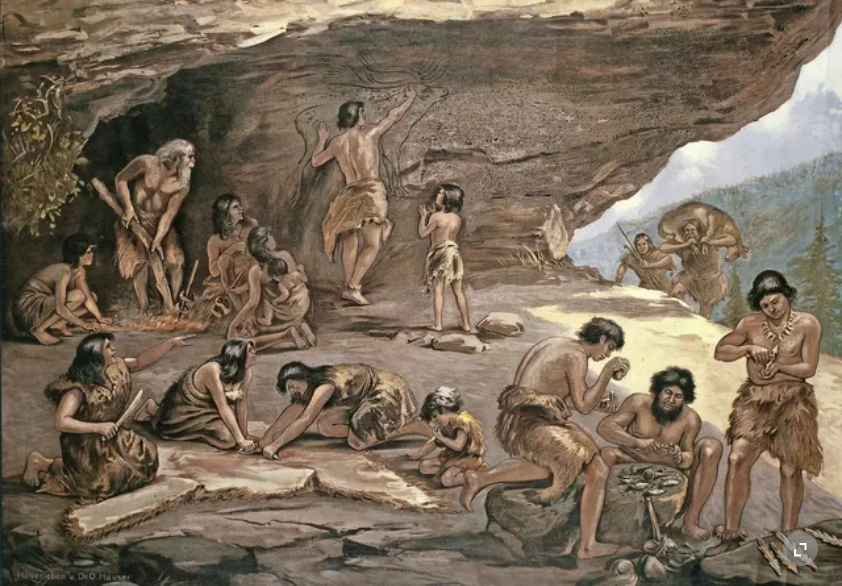
\includegraphics[width=0.8\textwidth,height=0.8\textheight]{media/image2.png}

}

\caption{\label{fig-hoehlenleben-zur-aelteren-steinzeit}Höhlenleben zur
älteren Steinzeit}

\end{figure}%

\begin{longtable}[]{@{}
  >{\raggedright\arraybackslash}p{(\columnwidth - 2\tabcolsep) * \real{0.0252}}
  >{\raggedright\arraybackslash}p{(\columnwidth - 2\tabcolsep) * \real{0.9748}}@{}}
\caption{Metadaten des Höhlenlebens zur älteren
Steinzeit}\label{tbl-metadaten-hoehlenleben-zur-aelteren-steinzeit}\tabularnewline
\toprule\noalign{}
\begin{minipage}[b]{\linewidth}\raggedright
Feldname
\end{minipage} & \begin{minipage}[b]{\linewidth}\raggedright
Wert
\end{minipage} \\
\midrule\noalign{}
\endfirsthead
\toprule\noalign{}
\begin{minipage}[b]{\linewidth}\raggedright
Feldname
\end{minipage} & \begin{minipage}[b]{\linewidth}\raggedright
Wert
\end{minipage} \\
\midrule\noalign{}
\endhead
\bottomrule\noalign{}
\endlastfoot
MediaId & m123415 \\
Filename & \\
Title & Höhlenleben zur älteren Steinzeit \\
Subject & Geschlechterbild, Geschlechterstereotyp,
Geschlechterverhältnis, Stigmatisierung, Kultur, Kunst \\
Description & Auf diesem Lebensbild wird eine strikte Arbeitsteilung
zwischen Mann und Frau dargestellt. Dabei ist der Mann für die Jagd
zuständig und die Frau für das Sammeln und die Kinderbetreuung. Auch die
materielle Kultur (u. a. Werkzeuge und Kunstgegenstände) wird primär von
Männern hergestellt. Obwohl die Zeichnung von Carl Arriens sehr alt ist
(sie entstand um 1900), finden sich ähnliche Szenarien bis weit in die
1990er Jahre. \\
Creator & Carl Ariens
\href{https://www.wikidata.org/wiki/Q15451450}{Q15451450} \\
Publisher & Universitätsbibliothek Heidelberg
\href{https://www.wikidata.org/wiki/Q880794}{Q880794} \\
Date & 1927 \\
Era & Frühgeschichte \\
Type & Image \\
Format & image/jpeg \\
Extent & 842 x 586 \\
Source & Inv. Nr. S 1985/2364 \\
Language & \\
Relation & \url{https://doi.org/10.11588/artdok.00008148} \\
Rights & CC BY-SA 4.0 DEED \\
License &
\url{https://creativecommons.org/licenses/by-sa/4.0/deed.de} \\
\end{longtable}

\paragraph{Sexualisierung der Frau}\label{sec-sexualisierung-der-frau}

\begin{figure}

\centering{

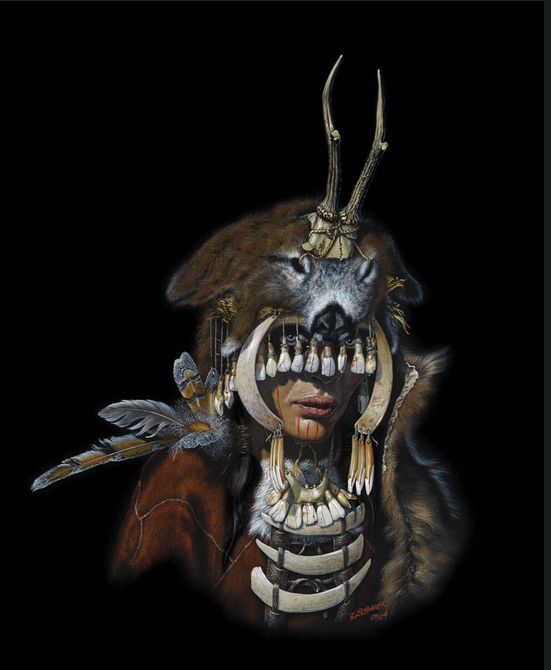
\includegraphics[width=0.8\textwidth,height=0.8\textheight]{media/image1.png}

}

\caption{\label{fig-bestattung-von-bad-duerrenberg}Bestattung von Bad
Dürrenberg}

\end{figure}%

\begin{longtable}[]{@{}
  >{\raggedright\arraybackslash}p{(\columnwidth - 2\tabcolsep) * \real{0.0108}}
  >{\raggedright\arraybackslash}p{(\columnwidth - 2\tabcolsep) * \real{0.9892}}@{}}
\caption{Metadaten der Bestattung von Bad
Dürrenberg}\label{tbl-metadaten-bestattung-von-bad-duerrenberg}\tabularnewline
\toprule\noalign{}
\begin{minipage}[b]{\linewidth}\raggedright
Feldname
\end{minipage} & \begin{minipage}[b]{\linewidth}\raggedright
Wert
\end{minipage} \\
\midrule\noalign{}
\endfirsthead
\toprule\noalign{}
\begin{minipage}[b]{\linewidth}\raggedright
Feldname
\end{minipage} & \begin{minipage}[b]{\linewidth}\raggedright
Wert
\end{minipage} \\
\midrule\noalign{}
\endhead
\bottomrule\noalign{}
\endlastfoot
MediaId & m123416 \\
Filename & \\
Title & Bestattung von Bad Dürrenberg \\
Subject & Sexismus, Ableismus , Tod \\
Description & Bei der Bestattung von Bad Dürrenberg handelt es sich um
ein etwa 9000 Jahre altes Grab. Darin wurde eine Frau zusammen mit einem
Säugling bestattet. Ihr wurde ein überreiches Grabinventar aus einer
Vielfalt an Tierknochen beigegeben, die vermutlich zu einem Collier,
einem Umhang oder einem Kopfschmuck gehörten. Die Frau war körperlich
stark behindert. So hatte sie unter anderem eine ausgeprägte Arthrose.
Sie starb zwischen 30 und 40 jährig an einer Sepsis aufgrund eines
Kieferabszesses, der ihre untere Gesichtshälfte entstellte. Das
Landesmuseum für Vorgeschichte in Halle berücksichtigt diese Faktoren
beim Lebensbild allesamt nicht. Bei diesem Beispiel handelt es sich um
eine Verzerrung einer historischen Realität, die durch die bildliche
Darstellung in einer Erotisierung mündet. Allgemein fehlen Darstellungen
von Menschen aus archäologischen Kontexten mit körperlicher oder
geistiger Behinderung in Lebensbildern, obwohl diese über
anthropologische oder genetische Analysen eindeutig belegt sind. \\
Creator & Landesamt für Denkmalpflege und Archäologie Sachsen-Anhalt
\href{https://www.wikidata.org/wiki/Q1802049}{Q1802049}, Karol
Schauer \\
Publisher & Landesamt für Denkmalpflege und Archäologie Sachsen-Anhalt
\href{https://www.wikidata.org/wiki/Q1802049}{Q1802049}, Karol
Schauer \\
Date & \\
Era & Frühgeschichte \\
Type & Image \\
Format & image/jpeg \\
Extent & 551 x 670 \\
Source & Landesamt für Denkmalpflege und Archäologie Sachsen-Anhalt
\href{https://www.wikidata.org/wiki/Q1802049}{Q1802049}, Karol
Schauer \\
Language & \\
Relation &
\url{https://www.landesmuseum-vorgeschichte.de/dauerausstellung/menschenwechsel/die-schamanin-von-bad-duerrenberg.html} \\
Rights & Karol Schauer \\
License &
\url{https://rightsstatements.org/page/InC-RUU/1.0/?language=de} \\
\end{longtable}

\subsubsection{Positive Beispiele von
Lebensbildern}\label{positive-beispiele-von-lebensbildern}

\paragraph{Opferplatz Thorberger Moor}\label{opferplatz-thorberger-moor}

\begin{figure}

\centering{

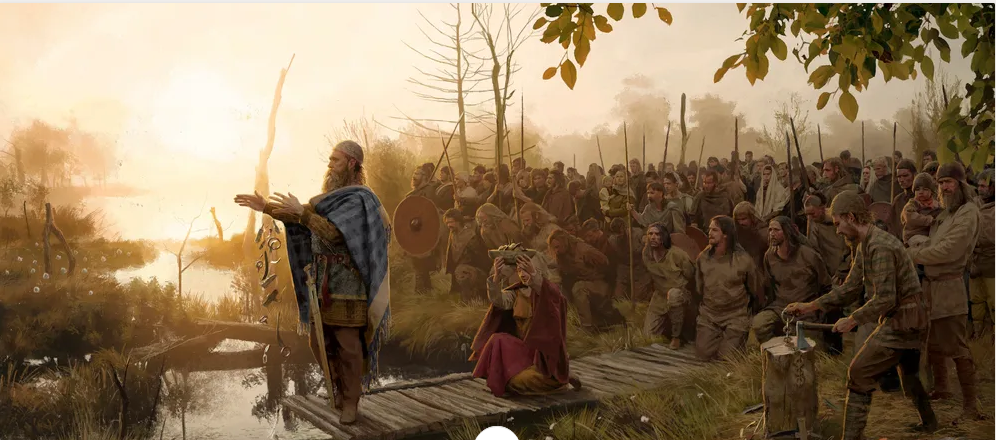
\includegraphics[width=0.8\textwidth,height=0.8\textheight]{media/image3.png}

}

\caption{\label{fig-opferplatz-thorberger-moor}Opferplatz Thorberger
Moor}

\end{figure}%

\begin{longtable}[]{@{}
  >{\raggedright\arraybackslash}p{(\columnwidth - 2\tabcolsep) * \real{0.0279}}
  >{\raggedright\arraybackslash}p{(\columnwidth - 2\tabcolsep) * \real{0.9721}}@{}}
\caption{Metadaten des Opferplatzes Thorberger
Moor}\label{tbl-metadaten-opferplatz-thorberger-moor}\tabularnewline
\toprule\noalign{}
\begin{minipage}[b]{\linewidth}\raggedright
Feldname
\end{minipage} & \begin{minipage}[b]{\linewidth}\raggedright
Wert
\end{minipage} \\
\midrule\noalign{}
\endfirsthead
\toprule\noalign{}
\begin{minipage}[b]{\linewidth}\raggedright
Feldname
\end{minipage} & \begin{minipage}[b]{\linewidth}\raggedright
Wert
\end{minipage} \\
\midrule\noalign{}
\endhead
\bottomrule\noalign{}
\endlastfoot
MediaId & m123417 \\
Filename & \\
Title & Opferplatz Thorberger Moor \\
Subject & Kinder, Opfer, Kultur, Spiritualität \\
Description & Das Lebensbild zum Opferplatz Thorberger Moor zeigt einen
Mann, der zerstörte Schätze einer besiegten Gruppe im Moor versenkt.
Dieser Ritus bedeutete eine Demütigung für die Besiegten. Die
Illustration ist eines der wenigen Bilder, auf dem relativ kleine Kinder
Teil einer Handlung sind, die als nicht-kindgerecht eingestuft wird.
Eines der Kinder wird dabei von einem Mann getragen. \\
Creator & Samson J. Goetze \\
Publisher & \\
Date & 2020 \\
Era & Frühgeschichte \\
Type & Image \\
Format & image/jpeg \\
Extent & 996 x 440 \\
Source & \\
Language & \\
Relation &
\url{https://www.geo.de/magazine/geo-magazin/40607-geo-nr-10-2020-die-germanen} \\
Rights & Samson J. Goetze \\
License &
\url{https://rightsstatements.org/page/InC-RUU/1.0/?language=de} \\
\end{longtable}

\paragraph{Alle unter einem Dach}\label{alle-unter-einem-dach}

\begin{figure}

\centering{

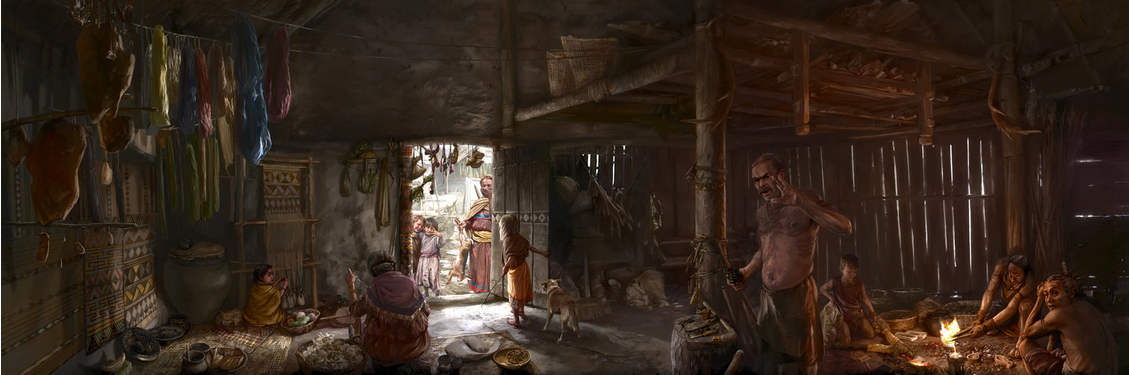
\includegraphics[width=0.8\textwidth,height=0.8\textheight]{media/image5.png}

}

\caption{\label{fig-alle-unter-einem-dach}Alle unter einem Dach}

\end{figure}%

\begin{longtable}[]{@{}
  >{\raggedright\arraybackslash}p{(\columnwidth - 2\tabcolsep) * \real{0.0370}}
  >{\raggedright\arraybackslash}p{(\columnwidth - 2\tabcolsep) * \real{0.9630}}@{}}
\caption{Metadaten von Alle unter einem
Dach}\label{tbl-metadaten-alle-unter-einem-dach}\tabularnewline
\toprule\noalign{}
\begin{minipage}[b]{\linewidth}\raggedright
Feldname
\end{minipage} & \begin{minipage}[b]{\linewidth}\raggedright
Wert
\end{minipage} \\
\midrule\noalign{}
\endfirsthead
\toprule\noalign{}
\begin{minipage}[b]{\linewidth}\raggedright
Feldname
\end{minipage} & \begin{minipage}[b]{\linewidth}\raggedright
Wert
\end{minipage} \\
\midrule\noalign{}
\endhead
\bottomrule\noalign{}
\endlastfoot
MediaId & m123418 \\
Filename & \\
Title & Alle unter einem Dach \\
Subject & Kinder, Familie, Sozialisation, Hausarbeit \\
Description & Das Lebensbild ``Alle unter einem Dach'' zeigt das Innere
eines spätbronzezeitlichen Hauses in einer Seeufersiedlung. Die Art der
Beziehungen unter den Personen ist nicht erkennbar. Das bedeutet, dass
es keine Kernfamilie gibt. Zudem sind die Kinder in die täglichen
Arbeiten eingebunden. \\
Creator & bunterhund \\
Publisher & bunterhund \\
Date & \\
Era & Frühgeschichte \\
Type & Image \\
Format & image/jpeg \\
Extent & 1129 x 375 \\
Source & \\
Language & \\
Relation & \url{https://bunterhund.ch/index.php?ds=827\#b} \\
Rights & bunterhund \\
License &
\url{https://creativecommons.org/licenses/by-sa/4.0/deed.de} \\
\end{longtable}

\paragraph{Die Keltin}\label{die-keltin}

\begin{figure}

\centering{

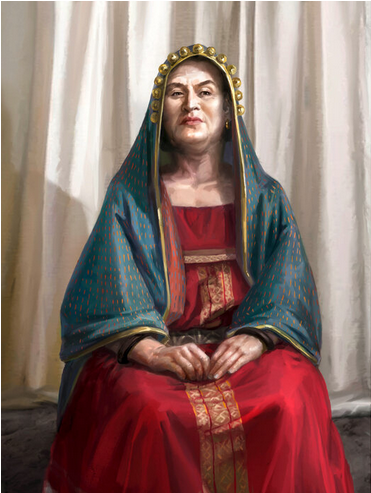
\includegraphics[width=0.8\textwidth,height=0.8\textheight]{media/image9.png}

}

\caption{\label{fig-die-keltin}Die Keltin}

\end{figure}%

\begin{longtable}[]{@{}
  >{\raggedright\arraybackslash}p{(\columnwidth - 2\tabcolsep) * \real{0.0186}}
  >{\raggedright\arraybackslash}p{(\columnwidth - 2\tabcolsep) * \real{0.9814}}@{}}
\caption{Metadaten der
Keltin}\label{tbl-metadaten-die-keltin}\tabularnewline
\toprule\noalign{}
\begin{minipage}[b]{\linewidth}\raggedright
Feldname
\end{minipage} & \begin{minipage}[b]{\linewidth}\raggedright
Wert
\end{minipage} \\
\midrule\noalign{}
\endfirsthead
\toprule\noalign{}
\begin{minipage}[b]{\linewidth}\raggedright
Feldname
\end{minipage} & \begin{minipage}[b]{\linewidth}\raggedright
Wert
\end{minipage} \\
\midrule\noalign{}
\endhead
\bottomrule\noalign{}
\endlastfoot
MediaId & m123419 \\
Filename & \\
Title & Die Keltin aus dem Prunkgrab von Ins \\
Subject & Frauen, Frauen in Führungspositionen, Frauenbild \\
Description & Die keltische Fürstin aus dem Fürstengrab von Ins hat
keine Idealfigur und ist grundsätzlich eine gute Antithese zum
Lebensbild der Bestattung von Bad Dürrenberg
Kapitel~\ref{sec-sexualisierung-der-frau}. Die Keltin wird mit einer
Aura der Autorität und Macht auf dem Lebensbild dargestellt. Sie
verkörpert die Rolle einer Entscheidungsträgerin, die über Leben und Tod
entscheiden kann. Der Begriff ``Fürstengrab'' kann auch mit
Prunkbestattungen des 6. bis 4. Jahrhunderts v.Chr. gleichgesetzt
werden. Solche Bestattungen sind vor allem in Frankreich, Süddeutschland
und der Schweiz bekannt. \\
Creator & bunterhund \\
Publisher & bunterhund \\
Date & \\
Era & Frühgeschichte \\
Type & Image \\
Format & image/jpeg \\
Extent & 371 x 493 \\
Source & \\
Language & \\
Relation &
\url{https://bunterhund.ch/index.php?dh1=0&dh2=&dh3=&ds=1716&\#b} \\
Rights & bunterhund \\
License &
\url{https://creativecommons.org/licenses/by-sa/4.0/deed.de} \\
\end{longtable}

\section{Literatur}\label{literatur}

\phantomsection\label{refs}
\begin{CSLReferences}{1}{0}
\bibitem[\citeproctext]{ref-australianresearchdatacommonsardc2020a}
Australian Research Data Commons (ARDC). 2020. {«{ARDC Metadata
Guide}»}, März. \url{https://doi.org/10.5281/ZENODO.6459832}.

\bibitem[\citeproctext]{ref-baca2016}
Baca, Murtha. 2016. \emph{Introduction to Metadata}. Herausgegeben von
Murtha Baca. 3. Aufl. Los Angeles: Getty Publications.
\url{http://www.getty.edu/publications/intrometadata}.

\bibitem[\citeproctext]{ref-carroll2021}
Carroll, Stephanie Russo, Edit Herczog, Maui Hudson, Keith Russell, und
Shelley Stall. 2021. {«Operationalizing the {CARE} and {FAIR Principles}
for {Indigenous} Data Futures»}. \emph{Scientific Data} 8 (1): 108.
\url{https://doi.org/10.1038/s41597-021-00892-0}.

\bibitem[\citeproctext]{ref-davis2021a}
Davis, Edie, und Bahareh Heravi. 2021. {«Linked {Data} and {Cultural
Heritage}: {A Systematic Review} of {Participation}, {Collaboration},
and {Motivation}»}. \emph{Journal on Computing and Cultural Heritage} 14
(2): 1--18. \url{https://doi.org/10.1145/3429458}.

\bibitem[\citeproctext]{ref-dogtas2022}
Doğtaş, Gürsoy, Marc-Paul Ibitz, Fatima Jonitz, Veronika Kocher, Astrid
Poyer, und Laurenz Stapf. 2022. {«Kritik an rassifizierenden und
diskriminierenden Titeln und Metadaten -- Praxisorientierte
Lösungsansätze»}. \emph{027.7 Zeitschrift für Bibliothekskultur /
Journal for Library Culture} 9 (4).
\url{https://doi.org/10.21428/1bfadeb6.abe15b5e}.

\bibitem[\citeproctext]{ref-freire2019a}
Freire, Nuno, Pável Calado, und Bruno Martins. 2019. {«Availability of
{Cultural Heritage Structured Metadata} in the {World Wide Web}»}. In
\emph{Connecting the {Knowledge Commons} --- {From Projects} to
{Sustainable Infrastructure}}, herausgegeben von Leslie Chan und Pierre
Mounier, 121--33. OpenEdition Press.
\url{https://doi.org/10.4000/books.oep.9024}.

\bibitem[\citeproctext]{ref-sgg2023}
Gabay, Simon, Tobias Hodel, Moritz Mähr, Stefan Nellen, Barbara
Roth-Lochner, Pascale Sutter, Andrea Voellmin, und Karin von Wartburg.
2023. {«Datenstandards Für Die Historische {Forschung} -- {Ein
White-Paper} Der {Schweizerischen Gesellschaft} Für {Geschichte}»}.
Herausgegeben von Schweizerische Gesellschaft für Geschichte.
\emph{Whitepaper}, November.
\url{https://doi.org/10.5281/ZENODO.10122052}.

\bibitem[\citeproctext]{ref-gruber2022a}
Gruber, Andrea. 2022. {«Vom Knüpfen feministischer Begriffsnetze:
Ariadnes Faden \& geschlechtersensible Normdaten»}. \emph{Mitteilungen
der Vereinigung Österreichischer Bibliothekarinnen und Bibliothekare} 75
(1): 262--88. \url{https://doi.org/10.31263/voebm.v75i1.7213}.

\bibitem[\citeproctext]{ref-heinrich2018}
Heinrich, Andreas, und Anita Runge. 2018. {«GenderOpen: Ein Repositorium
für die Geschlechterforschung»}. \url{https://doi.org/10.25595/584}.

\bibitem[\citeproctext]{ref-jaffeb}
Jaffe, Rachel. o.~J. {«Library {Guides}: {Metadata Creation}»}. Guide.
Zugegriffen 5. Mai 2024.
\url{https://guides.library.ucsc.edu/c.php?g=618773&p=4306381}.

\bibitem[\citeproctext]{ref-lampe2021}
Lampe, Moritz. 2021. \emph{Diskriminierende Begriffe und
Wissensordnungen im Bildarchiv}. Berliner handreichungen zur
bibliotheks- und informationswissenschaft 481. Berlin: Institut für
Bibliotheks- und Informationswissenschaft der Humboldt-Universität zu
Berlin. \url{https://doi.org/10.18452/23766}.

\bibitem[\citeproctext]{ref-sparber2016a}
Sparber, Sandra. 2016. {«What's the frequency, Kenneth? -- Eine
(queer)feministische Kritik an Sexismen und Rassismen im
Schlagwortkatalog»}. \emph{Mitteilungen der Vereinigung Österreichischer
Bibliothekarinnen und Bibliothekare} 69 (2): 236--43.
\url{https://doi.org/10.31263/voebm.v69i2.1629}.

\bibitem[\citeproctext]{ref-staunton2021}
Staunton, Ciara, Carlos Andrés Barragán, Stefano Canali, Calvin Ho,
Sabina Leonelli, Matthew Mayernik, Barbara Prainsack, und Ambroise
Wonkham. 2021. {«Open Science, Data Sharing and Solidarity: Who
Benefits?»} \emph{History and Philosophy of the Life Sciences} 43 (4):
115. \url{https://doi.org/10.1007/s40656-021-00468-6}.

\bibitem[\citeproctext]{ref-musis2024}
Team MusIS. o.~J. {«Regelwerke, Thesauri, Klassifikationen, Systematiken
und Begriffslisten»}. Wiki. BSZ Wiki. Zugegriffen 5. Mai 2024.
\url{https://wiki.bsz-bw.de/display/MUSIS/Regelwerke\%2C+Thesauri\%2C+Klassifikationen\%2C+Systematiken+und+Begriffslisten}.

\bibitem[\citeproctext]{ref-community2022a}
The Turing Way Community. 2022. {«The {Turing Way}: {A} Handbook for
Reproducible, Ethical and Collaborative Research»}.
\url{https://doi.org/10.5281/ZENODO.3233853}.

\bibitem[\citeproctext]{ref-wilkinson2016}
Wilkinson, Mark D., Michel Dumontier, IJsbrand Jan Aalbersberg,
Gabrielle Appleton, Myles Axton, Arie Baak, Niklas Blomberg, u.~a. 2016.
{«The {FAIR Guiding Principles} for Scientific Data Management and
Stewardship»}. \emph{Scientific Data} 3 (1): 160018.
\url{https://doi.org/10.1038/sdata.2016.18}.

\bibitem[\citeproctext]{ref-zhang2022a}
Zhang, Lei. 2022. {«Empowering Linked Data in Cultural Heritage
Institutions: {A} Knowledge Management Perspective»}. \emph{Data and
Information Management} 6 (3): 100013.
\url{https://doi.org/10.1016/j.dim.2022.100013}.

\end{CSLReferences}

\section{Anhang: Schlagwortindex GenderOpen inklusive
GND-Mapping}\label{sec-Schlagwortindex-GenderOpen}

\begin{longtable}[]{@{}
  >{\raggedright\arraybackslash}p{(\columnwidth - 8\tabcolsep) * \real{0.1707}}
  >{\raggedright\arraybackslash}p{(\columnwidth - 8\tabcolsep) * \real{0.3220}}
  >{\raggedright\arraybackslash}p{(\columnwidth - 8\tabcolsep) * \real{0.2146}}
  >{\raggedright\arraybackslash}p{(\columnwidth - 8\tabcolsep) * \real{0.1171}}
  >{\raggedright\arraybackslash}p{(\columnwidth - 8\tabcolsep) * \real{0.1756}}@{}}
\toprule\noalign{}
\begin{minipage}[b]{\linewidth}\raggedright
Open Gender-Term
\end{minipage} & \begin{minipage}[b]{\linewidth}\raggedright
\href{https://www.niso.org/schemas/iso25964}{ISO 25964-2} (MARC 7XX-\$4)
\end{minipage} & \begin{minipage}[b]{\linewidth}\raggedright
GND-Term
\end{minipage} & \begin{minipage}[b]{\linewidth}\raggedright
GND Identifier
\end{minipage} & \begin{minipage}[b]{\linewidth}\raggedright
Synonyme
\end{minipage} \\
\midrule\noalign{}
\endhead
\bottomrule\noalign{}
\endlastfoot
Ableismus & =EQ & Ableismus & 1276051255 & \\
Abtreibungsdebatte & & Not Found & Not Found & \\
Abtreibungsgegner & & Not Found & Not Found & \\
Abtreibungsverbot & & Not Found & Not Found & \\
Adoption & =EQ & Adoption & 4000522-7 & \\
Affekt & =EQ & Affekt & 4135470-9 & \\
Agency & EQ & Handlungskompetenz & 4125926-9 & Handlungskompetenz \\
AIDS & =EQ & Aids & 4112470-4 & \\
Aktivismus & =EQ & Aktivismus & 4000973-7 & \\
Alleinerziehende & EQ & Alleinerziehende Mutter & 4001238-4 & \\
Alleinlebende & EQ & Alleinstehender & 4001240-2 & \\
Allgemeines Gleichbehandlungsgesetz & =EQ & Allgemeines
Gleichbehandlungsgesetz & 7542750-3 & \\
Alltag & =EQ & Alltag & 4001307-8 & \\
Alter & =EQ & Alter & 4001446-0 & \\
Alterssicherung & \textasciitilde EQ & Altersversorgung & 4001479-4 &
Altersversorgung \\
Androgynie & BM & Androgynie & 4001967-6 & \\
Androzentrismus & =EQ & Androzentrismus & 1223001903 & \\
Anerkennung & =EQ & Anerkennung & 4128520-7 & \\
Antidiskriminierung & & Not Found & 1035294273 & \\
Antifaschismus & =EQ & Antifaschismus & 4122803-0 & \\
Antifeminismus & EQ\textbar{} & Frauenfeindlichkeit & 4155231-3 &
Frauenfeindlichkeit \\
Antirassismus & =EQ & Antirassismus & 4275311-9 & \\
Antisemitismus & =EQ & Antisemitismus & 1235847462 & \\
Antiziganismus & =EQ & Antiziganismus & 4808992-8 & \\
Arbeit & =EQ & Arbeit & 1136593101 & \\
Arbeitskampf & =EQ & Arbeitskampf & 4002702-8 & \\
Arbeitsmarkt & =EQ & Arbeitsmarkt & 4002733-8 & \\
Arbeitsteilung & =EQ & Arbeitsteilung & 4002787-9 & \\
Arbeitsverhältnis & =EQ & Arbeitsverhältnis & 4002799-5 & \\
Architektur & =EQ & Architektur & 4002851-3 & \\
Armut & =EQ & Armut & 1234066785 & \\
Ästhetik & =EQ & Ästhetik & 1207079987 & \\
Asyl & =EQ & Asyl & 4143260-5 & \\
Ausbeutung & =EQ & Ausbeutung & 4003677-7 & \\
Ausbildung & =EQ & Ausbildung & 4112628-2 & \\
Autonomie & =EQ & Autonomie & 1067437622 & \\
Begehren & =EQ & Begehren & 300735928 & \\
Behinderung & =EQ & Behinderung & 4112696-8 & \\
Beratung & =EQ & Beratung & 4005565-6 & \\
Beruf & =EQ & Beruf & 4005857-8 & \\
Berufstätigkeit & =EQ & Berufstätigkeit & 4069349-1 & \\
Berufsverbot & =EQ & Berufsverbot & 4005959-5 & \\
Berufswahl & =EQ & Berufswahl & 4005962-5 & \\
Beschneidung & EQ\textbar{} & Beschneidung oder Beschneidung & 7648122-0
oder 4144874-1 & Beschneidung  \\
Bevölkerung & =EQ & Bevölkerung & 4006287-9 & \\
Bewusstsein & =EQ & Bewusstsein & 4006349-5 & \\
Beziehung & =EQ & Beziehung & 4145198-3 & \\
Bildung & =EQ & Bildung & 1085646750 & \\
Bildungsarbeit & =EQ & Bildungsarbeit & 4112760-2 & \\
Bildungssystem & =EQ & Bildungssystem & 4069467-7 & \\
Biografieforschung & =EQ & Biografieforschung & 4132300-2 & \\
Biologie & =EQ & Biologie & 4006851-1 & \\
Biologismus & =EQ & Biologismus & 4232000-8 & \\
Biopolitik & =EQ & Biopolitik & 4137810-6 & \\
Bisexualität & =EQ & Bisexualität & 4006963-1 & \\
Care & =EQ & Care & 4648135-7 & \\
Chancengleichheit & =EQ & Chancengleichheit & 4009736-5 & \\
Christentum & =EQ & Christentum & 4010074-1 & \\
Coming-out & =EQ & Coming-out & 4300693-0 & \\
Computerspiel & =EQ & Computerspiel & 4010457-6 & \\
Cross-dressing & EQ & Crossdressing & 1103153943 & \\
Cyborg & =EQ & Cyborg & 4786457-6 & \\
DDR & EQ & Deutschland (DDR) & 4011890-3 & \\
Debatte & =EQ & Debatte & 4148952-4 & \\
Dekonstruktion & =EQ & Dekonstruktion & 4149032-0 & \\
Demografie & =EQ & Demographie & 4011412-0 & \\
Demokratie & =EQ & Demokratie & 4011413-2 & \\
Depression & =EQ & Depression & 4011474-0 & \\
Diaspora & =EQ & Diaspora & 1231305827 & \\
Dichotomie & =EQ & Dichotomie & 300727208 & \\
Dienstleistungssektor & =EQ & Dienstleistungssektor & 4012183-5 & \\
Digitalisierung & =EQ & Digitalisierung & 4123065-6 & \\
Diskriminierung & =EQ & Diskriminierung & 4012472-1 & \\
Diskurs & =EQ & Diskurs & 300471955 & \\
Disziplinarität & & Not Found & Not Found & \\
Diversität & RM & Heterogenität & 4201275-2 & Heterogenität \\
Diversity Management & =EQ & Diversity Management & 7611361-9 & \\
Doing Gender & & Not Found & Not Found & \\
Drag & =EQ & Drag & 1176239244 & \\
Ehe & =EQ & Ehe & 4013630-9 & \\
Ehegattensplitting & =EQ & Ehegattensplitting & 7503178-4 & \\
Ehrenamt & =EQ & Ehrenamt & 4121161-3 & \\
Eigentum & =EQ & Eigentum & 4013793-4 & \\
Einkommen & =EQ & Einkommen & 4013887-2 & \\
Eltern & =EQ & Eltern & 4014516-5 & \\
Elternschaft & =EQ & Elternschaft & 4152054-3 & \\
Emanzipation & =EQ & Emanzipation & 4130667-3 & \\
Entwicklung & =EQ & Entwicklung & 1171380917 & \\
Entwicklungszusammenarbeit & =EQ & Entwicklungszusammenarbeit &
4198756-1 & \\
Epistemologie & BM & Genetische Epistemologie & 4135354-7 & \\
Erfahrung & =EQ & Erfahrung & 1239135211 & \\
Erinnerungskultur & & Not Found & Not Found & \\
Ernährung & =EQ & Ernährung & 4015332-0 & \\
Erotik & =EQ & Erotik & 4015369-1 & \\
Erwachsenenbildung & =EQ & Erwachsenenbildung & 4015428-2 & \\
Erwerbsarbeit & EQ & Arbeit & 4002567-6 & \\
Erwerbslosigkeit & EQ & Arbeitslosigkeit & 4002730-2 &
Arbeitslosigkeit \\
Erwerbstätigkeit & EQ & Berufstätigkeit & 4069349-1 & \\
Erziehung & =EQ & Erziehung & 4015482-8 & \\
Essentialismus & =EQ & Essentialismus & 4113474-6 & \\
Essstörung & =EQ & Essstörung & 4113475-8 & \\
Ethik & =EQ & Ethik & 1088045626 & \\
Ethnizität & =EQ & Ethnizität & 4220764-2 & \\
Ethnozentrismus & =EQ & Ethnozentrismus & 4070982-6 & \\
Europäische Union & =EQ & Europäische Union & 5098525-5 & \\
Eurozentrismus & =EQ & Eurozentrismus & 4200132-8 & \\
Exil & =EQ & Exil & 1026311314 & \\
Familie & =EQ & Familie & 123631333X & \\
Familienbild & =EQ & Familienbild & 1103153382 & \\
Familienform & & Not Found & Not Found & \\
Familienpolitik & =EQ & Familienpolitik & 4016418-4 & \\
Faschismus & =EQ & Faschismus & 4016494-9 & \\
Female Genital Cutting & & Not Found & Not Found & \\
Female Genital Mutilation & & Not Found & Not Found & \\
Feminisierung & =EQ & Feminisierung & 4397368-1 & \\
Feminismus & =EQ & Feminismus & 4222126-2 & \\
Faschismus & & Not Found & Not Found & \\
Film & =EQ & Film & 4017102-4 & \\
Flucht & =EQ & Flucht & 1274267641 & \\
Frauen & =EQ & Frauen & 1142536149 & \\
Frauen in Führungspositionen & & Not Found & Not Found & \\
Frauenanteil & NM & Geschlechterverhältnis & 4243608-4 &
Geschlechterverhältnis  \\
Frauenbeauftragte & & Not Found & Not Found & \\
Frauenberuf & =EQ & Frauenberuf & 1201699207 & \\
Frauenbewegung & =EQ & Frauenbewegung & 4071428-7 & \\
Frauenbild & =EQ & Frauenbild & 4125057-6 & \\
Frauenfeindlichkeit & =EQ & Frauenfeindlichkeit & 4155231-3 & \\
Frauenförderung & =EQ & Frauenförderung & 4226107-7 & \\
Frauenforschung & =EQ & Frauenforschung & 4244891-8 & \\
Frauengeschichte & & Not Found & Not Found & \\
Frauenhaus & =EQ & Frauenhaus & 4155233-7 & \\
Frauenorganisation & EQ & Frauenverband & 4155246-5 & Frauenverband \\
Frauenpolitik & =EQ & Frauenpolitik & 4113623-8 & \\
Frauenrechte & & Not Found & Not Found & \\
Frauenstudium & =EQ & Frauenstudium & 4129623-0 & \\
Frauenuniversität & =EQ & Frauenuniversität & 4470659-5 & \\
Frauenwahlrecht & =EQ & Frauenwahlrecht & 120484805X & \\
Freundschaft & =EQ & Freundschaft & 4018480-8 & \\
Fundamentalismus & =EQ & Fundamentalismus & 4137178-1 & \\
Geburtenkontrolle & \textasciitilde EQ & Geburtenregelung & 4019593-4 &
Geburtenregelung \\
Gefühl & =EQ & Gefühl & 4019702-5 & \\
Gender & & Not Found & Not Found & \\
Gender Bias & & Not Found & Not Found & \\
Gender Budgeting & & Not Found & Not Found & \\
Gender Mainstreaming & =EQ & Gender Mainstreaming & 4845903-3 & \\
Gender Pay Gap & =EQ & Gender Pay Gap & 1314965875 & \\
Genderkompetenz & & Not Found & Not Found & \\
Generation & =EQ & Generation & 4259035-8 & \\
Genetik & =EQ & Genetik & 4071711-2 & \\
Genozid & EQ & Völkermord & 4063690-2 & Völkermord \\
Gentechnologie & =EQ & Gentechnologie & 4071722-7 & \\
Gerechtigkeit & =EQ & Gerechtigkeit & 4020310-4 & \\
Geschichte & =EQ & Geschichte & 4020517-4 & \\
Geschlecht & =EQ & Geschlecht & 4020547-2 & \\
Geschlechterbild & & Not Found & Not Found & \\
Geschlechterdifferenz & EQ & Geschlechterunterschied & 4071781-1 &
Geschlechterunterschied \\
Geschlechterforschung & =EQ & Geschlechterforschung & 4482930-9 & \\
Geschlechtergerechte Sprache & =EQ & Geschlechtergerechte Sprache &
1186727241 & \\
Geschlechterkonstruktion & & Not Found & Not Found & \\
Geschlechterordnung & & Not Found & Not Found & \\
Geschlechterrolle & =EQ & Geschlechterrolle & 4071776-8 & \\
Geschlechterstereotyp & =EQ & Geschlechterstereotyp & 4157010-8 & \\
Geschlechterverhältnis & =EQ & Geschlechterverhältnis & 4020548-4 & \\
Geschlechtsidentität & =EQ & Geschlechtsidentität & 4181116-1 & \\
Geschlechtsspezifik & & Not Found & Not Found & \\
Gesellschaft & =EQ & Gesellschaft & 4020588-5 & \\
Gesellschaftstheorie & RM & Soziologische Theorie & 4077628-1 &
Soziologische Theorie \\
Gesetz & =EQ & Gesetz & 4020660-9 & \\
Gesundheit & =EQ & Gesundheit & 4020754-7 & \\
Gewalt & =EQ & Gewalt & 4020832-1 & \\
Gewalt gegen Frauen & =EQ & Gewalt gegen Frauen & 7505777-3 & \\
Gewerkschaft & =EQ & Gewerkschaft & 4020872-2 & \\
Gleichberechtigung & =EQ & Gleichberechtigung & 4021216-6 & \\
Gleichheit & =EQ & Gleichheit & 4021231-2 & \\
Gleichstellungsbeauftragte & =EQ & Gleichstellungsbeauftragte &
4125418-1 & \\
Gleichstellungspolitik & NM & Geschlechterpolitik & 4556952-6 & \\
Globalisierung & =EQ & Globalisierung & 4557997-0 & \\
Habitus & =EQ & Habitus & 1162075538 & \\
Haft & =EQ & Haft & 4327862-0 & \\
Hass & =EQ & Haß & 1117937836 & \\
Hausarbeit & =EQ & Hausarbeit & 4023699-7 & \\
Hausfrau & =EQ & Hausfrau & 4023733-3 & \\
Hegemonie & =EQ & Hegemonie & 4023979-2 & \\
Heimat & =EQ & Heimat & 1227062958 & \\
Hermaphroditismus & =EQ & Hermaphroditismus & 4117739-3 & \\
Herrschaft & =EQ & Herrschaft & 1310677700 & \\
Heterogenität & =EQ & Heterogenität & 4201275-2 & \\
Heteronormativität & =EQ & Heteronormativität & 1227961537 & \\
Heterosexualität & =EQ & Heterosexualität & 4159748-5 & \\
Heterosexuelle Matrix & & Not Found & Not Found & \\
Hierarchie & =EQ & Hierarchie & 4024842-2 & \\
Hirnforschung & =EQ & Hirnforschung & 4123382-7 & \\
HIV & =EQ & HIV & 4200792-6 & \\
Hochschule & =EQ & Hochschule & 4072560-1 & \\
Homofeindlichkeit & EQ & Homophobie & 4688835-4 & Homophobie \\
Homosexualität & =EQ & Homosexualität & 4025798-8 & \\
Identität & =EQ & Identität & 4026482-8 & \\
Ideologie & =EQ & Ideologie & 4026486-5 & \\
Individualisierung & =EQ & Individualisierung & 4161542-6 & \\
Individuum & =EQ & Individuum & 4026751-9 & \\
Industrie & =EQ & Industrie & 4026779-9 & \\
Informatik & =EQ & Informätik & 10322792-1 & \\
Inklusion & BM & Inklusion & 4696474-5 & \\
Institution & BM & Institution & 4027207-2 & \\
Institutionalisierung & =EQ & Institutionalisierung & 4127678-4 & \\
Integration & =EQ & Integration & 1072506661 & \\
Interdependenz & =EQ & Interdependenz & 4114036-9 & \\
Interdisziplinarität & =EQ & Interdisziplinarität & 4449808-1 & \\
Interkulturalität & =EQ & Interkulturalität & 4519498-1 & \\
Internet & =EQ & Internet & 1186913827 & \\
Intersektionalität & =EQ & Intersektionalität & 7729679-5 & \\
Intersexualität & =EQ & Intersexualität & 4027484-6 & \\
Intervention & =EQ & Intervention & 1180525124 & \\
Intimität & =EQ & Intimsphäre & 4072909-6 & \\
Islam & =EQ & Islam & 4027743-4 & \\
Judentum & =EQ & Judentum & 4114087-4 & \\
Jugend & =EQ & Jugend & 4028859-6 & \\
Jugendliche & NM & Jugend & 4028859-6 & Jugend \\
Jungen & EQ & Junge & 4029002-5 & Junge \\
Jungenarbeit & =EQ & Jungenarbeit & 7506212-4 & \\
Kapitalismus & =EQ & Kapitalismus & 4029577-1 & \\
Karriere & =EQ & Karriere & 4073274-5 & \\
Kinder & =EQ & Kinder & 1219024597 & \\
Kinderbetreuung & =EQ & Kinderbetreuung & 4278357-4 & \\
Kindheit & =EQ & Kindheit & 112666958X & \\
Kirche & =EQ & Kirche & 4030702-5 & \\
Klasse & =EQ & Klasse & 1228896208 & \\
Kleidung & =EQ & Kleidung & 4031011-5 & \\
Koedukation & =EQ & Koedukation & 4031467-4 & \\
Kolonialismus & =EQ & Kolonialismus & 4073624-6 & \\
Kommunikation & =EQ & Kommunikation & 300621787 & \\
Konflikt & =EQ & Konflikt & 1138451614 & \\
Konstruktivismus & BM & Konstruktivismus & 4639653-6 & \\
Konsum & EQ & Verbrauch & 4078777-1 & Verbrauch \\
Konzentrationslager & =EQ & Konzentrationslager & 4032352-3 & \\
Kopftuch & =EQ & Kopftuch & 4195492-0 & \\
Körper & =EQ & Körper & 4031575-7 & \\
Krankenpflege & =EQ & Krankenpflege & 4032813-2 & \\
Krankheit & =EQ & Krankheit & 1235355772 & \\
Krieg & =EQ & Krieg & 4033114-3 & \\
Kriminalität & =EQ & Kriminalität & 4033178-7 & \\
Krise & =EQ & Krise & 1310230021 & \\
Kritik & =EQ & Kritik & 4033229-9 & \\
Kritische Theorie & =EQ & Kritische Theorie & 4073840-1 & \\
Kultur & =EQ & Kultur & 4125698-0 & \\
Kunst & =EQ & Kunst & 1274253799 & \\
Landwirtschaft & =EQ & Landwirtschaft & 4034402-2 & \\
Lebensbedingungen & =EQ & Lebensbedingungen & 4130642-9 & \\
Lebensform & =EQ & Lebensform & 4034863-5 & \\
Lebensgemeinschaft & =EQ & Lebensgemeinschaft & 4167021-8 & \\
Lebenspartnerschaft & EQ & Eingetragene Lebenspartnerschaft & 4648252-0
& \\
Lehre & =EQ & Lehre & 7573711-5 & \\
Leib & =EQ & Leib & 1225568218 & \\
Lesben & EQ & Lesbe & 4035430-1 & Lesbe \\
Lesbenbewegung & & Not Found & Not Found & \\
Liberalismus & =EQ & Liberalismus & 4035582-2 & \\
Liebe & =EQ & Liebe & 1228569932 & \\
Literatur & =EQ & Literatur & 1248794494 & \\
Lohn & =EQ & Lohn & 2018391-4 & \\
LSBTIQ & & Not Found & Not Found & \\
Macht & =EQ & Macht & 1123508909 & \\
Mädchen & =EQ & Mädchen & 1262354552 & \\
Mädchenarbeit & =EQ & Mädchenarbeit & 7506089-9 & \\
Männer & =EQ & Männer & 1189215802 & \\
Männerbild & =EQ & Männerbild & 4139085-4 & \\
Männerbund & =EQ & Männerbund & 4168466-7 & \\
Männlichkeit & =EQ & Männlichkeit & 4123701-8 & \\
Marginalisierung & & Not Found & Not Found & \\
Mathematik & =EQ & Mathematik & 4037944-9 & \\
Matriarchat & =EQ & Matriarchat & 4037966-8 & \\
Medien & =EQ & Medien & 4169187-8 & \\
Medizin & =EQ & Medizin & 4038243-6 & \\
Menschenbild & =EQ & Menschenbild & 4074722-0 & \\
Menschenhandel & =EQ & Menschenhandel & 4125897-6 & \\
Menschenrechte & =EQ & Menschenrechte & 300689543 & \\
Migration & =EQ & Migration & 300752466 & \\
Milieu & =EQ & Milieu & 4074798-0 & \\
Militär & =EQ & Militär & 4039305-7 & \\
Minderheit & =EQ & Minderheit & 4752223-9 & \\
MINT & =EQ & MINT & 1065095619 & \\
Misshandlung & =EQ & Misshandlung & 4170137-9 & \\
Mobilität & =EQ & Mobilität & 4039785-3 & \\
Mode & =EQ & Mode & 4039792-0 & \\
Moderne & =EQ & Moderne & 4039827-4 & \\
Moral & =EQ & Moral & 1276103034 & \\
Musik & =EQ & Musik & 125914528X & \\
Mütter & =EQ & Mutter & 4040949-1 & \\
Mutterbild & =EQ & Mutterbild & 4170889-1 & \\
Mütterlichkeit & \textasciitilde EQ & Das Mütterliche & 4131108-5 & Das
Mütterliche \\
Mutterschaft & =EQ & Mutterschaft & 4140725-8 & \\
Mythos & =EQ & Mythos & 4075159-4 & \\
Nachhaltigkeit & =EQ & Nachhaltigkeit & 4326464-5 & \\
Nationalismus & =EQ & Nationalismus & 4041300-7 & \\
Nationalsozialismus & =EQ & Nationalsozialismus & 4041316-0 & \\
Nationalstaat & =EQ & Nationalstaat & 4041331-7 & \\
Natur & =EQ & Natur & 1255124717 & \\
Neoliberalismus & =EQ & Neoliberalismus & 4171438-6 & \\
Netzwerk & =EQ & Netzwerk & 300131852 & \\
Nichtregierungsorganisation & EQ+ & Nichtstaatliche Organisation &
4131014-7 & Nichtstaatliche Organisation \\
Normen & =EQ & Normen & 1168177278 & \\
Objektivität & =EQ & Objektivität & 4172310-7 & \\
Öffentlichkeit & =EQ & Öffentlichkeit & 4043183-6 & \\
Ökologie & =EQ & Ökologie & 4043207-5 & \\
Ontologie & =EQ & Ontologie & 1130186792 & \\
Opfer & =EQ & Opfer & 4434480-6 & \\
Organisation & =EQ & Organisation & 4043774-7 & \\
Pädagogik & =EQ & Pädagogik & 4044302-4 & \\
Partizipation & =EQ & Partizipation & 4044789-3 & \\
Patriarchat & =EQ & Patriarchat & 4044914-2 & \\
People of Color & EQ & Person of Color & 4034855-6 & \\
Performativität & BM & Performativität & 7651115-7 & \\
Philosophie & =EQ & Philosophie & 4045791-6 & \\
Physik & =EQ & Physik & 4045956-1 & \\
Politik & =EQ & Politik & 4046514-7 & \\
Pornografie & =EQ & Pornografie & 4046809-4 & \\
Postkoloniale Theorie & & Not Found & Not Found & \\
Postkolonialismus & =EQ & Postkolonialismus & 4566658-1 & \\
Postmoderne & =EQ & Postmoderne & 4115604-3 & \\
Poststrukturalismus & =EQ & Poststrukturalismus & 4137176-8 & \\
Prävention & =EQ & Prävention & 4076308-0 & \\
Prekarisierung & =EQ & Prekarisierung & 128564378X & \\
Presse & =EQ & Presse & 4047150-0 & \\
Privatheit & =EQ & Privatheit & 4195103-7 & \\
Professionalisierung & =EQ & Professionalisierung & 4047376-4 & \\
Prostitution & =EQ & Prostitution & 4047516-5 & \\
Psychiatrie & =EQ & Psychiatrie & 108057249X & \\
Psychoanalyse & =EQ & Psychoanalyse & 4047689-3 & \\
Pubertät & =EQ & Pubertät & 4047762-9 & \\
Qualifikation & =EQ & Qualifikation & 4125835-6 & \\
Queer & =EQ & Queer & 1198894873 & \\
Queer Theory & EQ & Queer-Theorie & 7628620-4 & \\
Rassismus & =EQ & Rassismus & 4076527-1 & \\
Raum & =EQ & Raum & 1061812227 & \\
Recht & =EQ & Recht & 1190300982 & \\
Rechtsextremismus & & Not Found & Not Found & \\
Reisen & =EQ & Reisen & 1079282084 & \\
Religion & =EQ & Religion & 4049396-9 & \\
Repräsentation & =EQ & Repräsentation & 4137492-7 & \\
Reproduktion & =EQ & Reproduktion & 4115749-7 & \\
Reproduktionstechnologie & \textasciitilde EQ & Reproduktionsmedizin &
4197011-1 & Reproduktionsmedizin \\
Säkularismus & =EQ & Säkularismus & 4463409-2 & \\
Scham & =EQ & Scham & 1261599608 & \\
Scheidung & =EQ & Scheidung & 1140154451 & \\
Schule & =EQ & Schule & 4053474-1 & \\
Schwangerschaft & =EQ & Schwangerschaft & 4053724-9 & \\
Schwangerschaftsabbruch & =EQ & Schwangerschaftsabbruch & 4053732-8 & \\
Schwarze Deutsche & & Not Found & Not Found & \\
Schwule & EQ+ & Homosexuelles Paar & 4120463-3 & Homosexuelles Paar \\
Schwulenbewegung & EQ & Homosexuellenbewegung & 4140613-8 & \\
Selbstständigkeit & =EQ & Selbstständigkeit & 4137544-0 & \\
Sexarbeit & EQ & Prostitution & 4047516-5 & Prostitution \\
Sex-Gender-Debatte & & Not Found & Not Found & \\
Sexismus & =EQ & Sexismus & 4116483-0 & \\
Sexualisierte Gewalt & =EQ & Sexualisierte Gewalt & 1253967660 & \\
Sexualität & =EQ & Sexualität & 4054684-6 & \\
Sexuelle Belästigung & =EQ & Sexuelle Belästigung & 4238118-6 & \\
Shoah & EQ & Judenvernichtung & 4073091-8 & Judenvernichtung \\
Sklaverei & =EQ & Sklaverei & 4055260-3 & \\
Solidarität & =EQ & Solidarität & 4055429-6 & \\
Sorgearbeit & EQ & Care-Arbeit & 1163689106 & Care-Arbeit \\
Sozialarbeit & =EQ & Sozialarbeit & 4055676-1 & \\
Soziale Arbeit & EQ & Studiengang Soziale Arbeit & 7697887-4 & \\
Soziale Bewegung & =EQ & Soziale Bewegung & 4055707-8 & \\
Soziale Lage & EQ & Soziale Situation & 4077575-6 & Soziale Situation \\
Soziale Medien & EQ & Social Media & 4639271-3 & Social Media \\
Soziale Ungleichheit & =EQ & Soziale Ungleichheit & 4055736-4 & \\
Sozialisation & =EQ & Sozialisation & 4055783-2 & \\
Sozialismus & =EQ & Sozialismus & 4055785-6 & \\
Sozialleistung & =EQ & Sozialleistungen & 4055856-3 & \\
Sozialpolitik & =EQ & Sozialpolitik & 4055879-4 & \\
Sozialstruktur & =EQ & Sozialstruktur & 4055898-8 & \\
Spiel & =EQ & Spiel & 300550596 & \\
Spiritualität & =EQ & Spiritualität & 4116568-8 & \\
Sport & =EQ & Sport & 1057991643 & \\
Sprache & =EQ & Sprache & 1268136476 & \\
Staat & =EQ & Staat & 4056618-3 & \\
Stadt & =EQ & Stadt & 4056723-0 & \\
Stigmatisierung & =EQ & Stigmatisierung & 4057561-5 & \\
Strukturalismus & =EQ & Strukturalismus & 4058129-9 & \\
Subjekt & BM & Subjekt & 4183903-1 & \\
Subjektivierung & BM & Subjektivierung & 4747204-2 & \\
Subjektivität & =EQ & Subjektivität & 4058323-5 & \\
Sucht & =EQ & Sucht & 4058361-2 & \\
Tabu & =EQ & Tabu & 1132272548 & \\
Täter & =EQ & Täter & 4058881-6 & \\
Täterin & =EQ & Täterin & 4065027-3 & \\
Technik & =EQ & Technik & 4059205-4 & \\
Technologie & =EQ & Technologie & 4059276-5 & \\
Teilzeitarbeit & =EQ & Teilzeitbeschäftigung & 4078190-2 & \\
Terrorismus & =EQ & Terrorismus & 4059534-1 & \\
Theater & =EQ & Theater & 4059702-7 & \\
Theorie & =EQ & Theorie & 4059787-8 & \\
Therapie & =EQ & Therapie & 4059798-2 & \\
Tier & =EQ & Tier & 300839758 & \\
Tod & =EQ & Tod & 1092466800 & \\
Trans & =EQ & Trans & 300322577 & \\
Transdisziplinarität & =EQ & Transdisziplinarität & 4754633-5 & \\
Transformation & =EQ & Transformation & 4451062-7 & \\
Transgender & =EQ & Transgender & 7619945-9 & \\
Transsexualität & =EQ & Transsexualität & 4185937-6 & \\
Umwelt & =EQ & Umwelt & 1199664804 & \\
unbezahlte Arbeit & & Not Found & Not Found & \\
Undoing Gender & & Not Found & Not Found & \\
Universalismus & =EQ & Universalismus & 4186917-5 & \\
Universität & =EQ & Universität & 4061778-6 & \\
Unternehmen & =EQ & Unternehmen & 4061963-1 & \\
Unterricht & =EQ & Unterricht & 1252487681 & \\
Utopie & =EQ & Utopie & 4041251-9 & \\
Väter & =EQ & Vater & 4062386-5 & \\
Vaterschaft & =EQ & Vaterschaft & 4187441-9 & \\
Vereinbarkeit & EQ & Kompatibilität & 4221530-4 & Kompatibilität \\
Verfolgung & =EQ & Verfolgung & 4127664-4 & \\
Vergeschlechtlichung & & Not Found & Not Found & \\
Vergewaltigung & =EQ & Vergewaltigung & 1119833566 & \\
Verhütung & BM & (Verhütungsring) & 121526982X & (Verhütungsring) \\
Verletzbarkeit & =EQ & Verwundbarkeit & 4188166-7 & Verwundbarkeit \\
Verschleierung & =EQ & Verschleierung & 4353166-0 & \\
Verwaltung & =EQ & Verwaltung & 4063317-2 & \\
Verwandtschaft & =EQ & Verwandtschaft & 4133957-5 & \\
Virtuelle Realität & =EQ & Virtuelle Realität & 4399931-1 & \\
Wandel & =EQ & Wandel & 1161346732 & \\
Weiblichkeit & =EQ & Weiblichkeit & 4079101-4 & \\
Weiterbildung & =EQ & Weiterbildung & 4117622-4 & \\
Werbung & =EQ & Werbung & 4065541-6 & \\
Widerstand & =EQ & Widerstand & 4079262-6 & \\
Wirtschaft & =EQ & Wirtschaft & 4066399-1 & \\
Wissen & =EQ & Wissen & 4066559-8 & \\
Wissenschaft & =EQ & Wissenschaft & 4066562-8 & \\
Wohlfahrtsstaat & =EQ & Wohlfahrtsstaat & 4117641-8 & \\
Wohnen & =EQ & Wohnen & 4066749-2 & \\
Xenophobie & =EQ & Fremdenfeindlichkeit & 4244141-9 &
Fremdenfeindlichkeit \\
Zeit & =EQ & Zeit & 4067461-7 & \\
Zuschreibung & =EQ & Zuschreibung & 4132036-0 & \\
Zwang & =EQ & Zwang & 138580839 & \\
\end{longtable}



\end{document}
